%%%%%%%%%%%%%%%%%%%%%%%%%%%%%%%%%%%%%%%%%%%%%%%%%%%%%%%%%%%%%%%%%%%%%%%%%%%%%%%%%%%%%%%%%%%%%%%%%%%
%%%%%%%%%%%%%%%%%%%%%%%%%%%%%%%%%%%%%%%%%%%%%%%%%%%%%%%%%%%%%%%%%%%%%%%%%%%%%%%%%%%%%%%%%%%%%%%%%%%

%\documentclass[12pt,letterpaper,draft]{book}
\documentclass[12pt,letterpaper]{book}
\usepackage[utf8]{inputenc}
\usepackage[spanish]{babel}

% para poner el tamano de los margenes
\usepackage[left=4cm,top=4cm,right=2.5cm,bottom=2.5cm]{geometry}

% para poner doble espacio
\usepackage{setspace}
\onehalfspacing

% util para revisar detalles finos, descativar despues
%\usepackage{layouts}

% para que escriba 'Figura...' en negritas
\usepackage[labelfont=bf]{caption}

% numeros con punto decimal (el default es coma decimal)
\decimalpoint

% tienen algunos comandos que ocupo, como align o defn
\usepackage{amsmath}
\usepackage{amsfonts}
\usepackage{amssymb}
\usepackage{amsthm}

% sin este no se pueden incluir imagenes
\usepackage{graphicx}

% sobre el formato de las paginas
\usepackage{cmap}
\pagestyle{plain}

% para importar el codigo de R y que se vea bien
\usepackage{listings}
\usepackage{color}

% este paquete pone las fracciones bonitas
\usepackage{nicefrac}

% hipervinculos a internet
\usepackage{url}

% para poner imagenes verticales en pagina completa
\usepackage{pdflscape}
\usepackage{afterpage}
\usepackage{everypage}
\usepackage{environ}

% tablas a hoja completa
\usepackage{tabularx}

% tablas con lineas gruesas
\usepackage{booktabs}

% grandes cantidades de codigo como comentario
\usepackage{verbatim}

% para que no se muevan mucho las figuras y tablas
\usepackage[section]{placeins}

% etiquetas en un multiplot
%\usepackage[caption=false]{subfig}
\usepackage{float}

% para que el indice tenga hipervinculos
\usepackage[pdftex,
            pdfauthor={Enciso Alva Julio Cesar},
            pdftitle={Tesis: Estacionariedad en PSG de AM como macador de PDC},
            pdfsubject={Matemáticas Aplicadas},
            %pdfkeywords={PALABRAS CLAVE},
            pdfproducer={Latex en Linux},
            pdfcreator={pdflatex}]{hyperref}

% para que la bibliografia aparezca en el indice
\usepackage[nottoc]{tocbibind}

% opciones de la bibliografia en espanol
\usepackage{babelbib}

% para tablas de colores
\usepackage{xcolor,colortbl}
\usepackage{multirow}

% arreglar problemas con las etiquetas con archivos multiples
\usepackage{xr}
\usepackage{zref}

% para poner palomita y tache
\usepackage{pifont}

% usar la F bonita para la tr de Fourier
\usepackage{mathrsfs}

% para escribir pseudocodigo
%\usepackage[spanish,onelanguage,linesnumbered,vlined]{algorithm2e}
\usepackage[spanish,onelanguage,linesnumbered,ruled,vlined]{algorithm2e}
% boxed

% para que aparezcan bien microvolt
\usepackage{siunitx}

% para que no haya espacio de sobra despues de las tablas
\usepackage{tabularx}

% resuelve el problema del espacio despues de as abreviaciones \newcommand
\usepackage{xspace}

% usar figuras de varias paginas
\usepackage[label font=bf]{subcaption}

% textsc + textbf
\usepackage{bold-extra}

%%%%%%%%%%%%%%%%%%%%%%%%%%%%%%%%%%%%%%%%%%%%%%%%%%%%%%%%%%%%%%%%%%%%%%%%%%%%%%%%%%%%%%%%%%%%%%%%%%%
%%%%%%%%%%%%%%%%%%%%%%%%%%%%%%%%%%%%%%%%%%%%%%%%%%%%%%%%%%%%%%%%%%%%%%%%%%%%%%%%%%%%%%%%%%%%%%%%%%%

% ajustando las figuras, parametros globales
%\renewcommand{\fps@figure}{!b}
%\renewcommand{\fps@table}{!b}

%%%%%%%%%%%%%%%%%%%%%%%%%%%%%%%%%%%%%%%%%%%%%%%%%%%%%%%%%%%%%%%%%%%%%%%%%%%%%%%%%%%%%%%%%%%%%%%%%%%
%%%%%%%%%%%%%%%%%%%%%%%%%%%%%%%%%%%%%%%%%%%%%%%%%%%%%%%%%%%%%%%%%%%%%%%%%%%%%%%%%%%%%%%%%%%%%%%%%%%

% comandos para tablas/figuras en hoja completa: SidewaysTable y SidewaysFigure

\newcounter{abspage}% \thepage not reliab

\makeatletter
\newcommand{\newSFPage}[1]% #1 = \theabspage
  {\global\expandafter\let\csname SFPage@#1\endcsname\null}

\NewEnviron{SidewaysFigure}{
\begin{figure}[p]
\protected@write\@auxout{\let\theabspage=\relax}% delays expansion until shipout
  {\string\newSFPage{\theabspage}}%
\ifdim\textwidth=\textheight
  \rotatebox{90}{\parbox[c][\textwidth][c]{\linewidth}{\BODY}}%
\else
  \rotatebox{90}{\parbox[c][\textwidth][c]{\textheight}{\BODY}}%
\fi
\end{figure}}

\NewEnviron{SidewaysTable}{
\begin{table}[p]
\bordes{1.1}
\protected@write\@auxout{\let\theabspage=\relax}% delays expansion until shipout
  {\string\newSFPage{\theabspage}}%
\ifdim\textwidth=\textheight
  \rotatebox{90}{\parbox[c][\textwidth][c]{\linewidth}{\BODY}}%
\else
  \rotatebox{90}{\parbox[c][\textwidth][c]{\textheight}{\BODY}}%
\fi
\end{table}}

%%%%%%%%%%%%%%%%%%%%%%%%%%%%%%%%%%%%%%%%%%%%%%%%%%%%%%%%%%%%%%%%%%%%%%%%%%%%%%%%%%%%%%%%%%%%%%%%%%%
%%%%%%%%%%%%%%%%%%%%%%%%%%%%%%%%%%%%%%%%%%%%%%%%%%%%%%%%%%%%%%%%%%%%%%%%%%%%%%%%%%%%%%%%%%%%%%%%%%%

\newcommand{\abbrlabel}[1]{\makebox[3cm][l]{\textbf{#1}\ \dotfill}}
\newenvironment{abbreviations}{\begin{list}{}{\renewcommand{\makelabel}{\abbrlabel}}}{\end{list}}

\pagestyle{plain}

%%%%%%%%%%%%%%%%%%%%%%%%%%%%%%%%%%%%%%%%%%%%%%%%%%%%%%%%%%%%%%%%%%%%%%%%%%%%%%%%%%%%%%%%%%%%%%%%%%%
%%%%%%%%%%%%%%%%%%%%%%%%%%%%%%%%%%%%%%%%%%%%%%%%%%%%%%%%%%%%%%%%%%%%%%%%%%%%%%%%%%%%%%%%%%%%%%%%%%%

% munchas abreviaciones que uso para ahorrar codigo, quiza ponga mas

\newtheorem{definicion}{Definición}[chapter]
\newtheorem{teorema}{Teorema}[chapter]
\newtheorem{proposicion}{Proposición}[chapter]
\newtheorem{demostracion}{Demostración}[chapter]
\newtheorem{observacion}{Observación}[chapter]

\newcommand{\R}{\mathbb{R}}
\newcommand{\C}{\mathbb{C}}
\newcommand{\N}{\mathbb{N}}
\newcommand{\Z}{\mathbb{Z}}
\newcommand{\intR}{\int_{-\infty}^{\infty}}
\newcommand{\intZ}{\int_{-\infty}^{0}}
\newcommand{\intPI}{\int_{-\pi}^{\pi}}
\newcommand{\simint}[1]{\int_{- #1 }^{ #1 }}
\newcommand{\prima}{^{\prime}}

\newcommand{\ddd}{$\delta$}
\newcommand{\dirac}{$\delta$  de Dirac}

\newcommand{\aste}[1]{\widehat{ #1 }^{\star}}
\newcommand{\est}[1]{\widehat{ #1 }}

\newcommand{\COS}[1]{\mathrm{cos}\left( #1 \right)}
\newcommand{\SEN}[1]{\mathrm{sen}\left( #1 \right)}

\newcommand{\E}[1]{\mathrm{E}\left[ #1 \right]}
\newcommand{\Var}[1]{\mathrm{Var}\left( #1 \right)}
\newcommand{\Cov}[1]{\mathrm{Cov}\left( #1 \right)}
\newcommand{\abso}[1]{\left| #1 \right|}

\newcommand{\xt}{$\{X(t)\}_{t\in \mathcal{T}}$ }
\newcommand{\xtd}{$\{x_t\}_{t=0,\dots,N}$ }
\newcommand{\orden}{\mathcal{O}}

\newcommand{\talque}{\mathrel{}\middle|\mathrel{}}

\newcommand{\lp}{\ell^{p}}
\newcommand{\llp}{L^{p}}
\newcommand{\ldos}{\ell^{2}}
\newcommand{\lldos}{L^{2}_I}

\newcommand{\sip}{\ding{51}}
\newcommand{\nop}{\ding{55}}

\newcommand{\pz}{\phantom{.0}}
\newcommand{\ppu}{\phantom{1}}
\newcommand{\phm}{\phantom{-}}

\newcommand{\hz}{\si{\hertz}\xspace}
\newcommand{\mv}{\si{\micro\volt}\xspace}

\newcommand{ \lento }{$\text{R}_{\text{E}}$\xspace}

\DeclareMathOperator{\argmax}{arg\,max}

\newcommand{\wdd}{\omega^{\star}}

%%%%%%%%%%%%%%%%%%%%%%%%%%%%%%%%%%%%%%%%%%%%%%%%%%%%%%%%%%%%%%%%%%%%%%%%%%%%%%%%%%%%%%%%%%%%%%%%%%%
%%%%%%%%%%%%%%%%%%%%%%%%%%%%%%%%%%%%%%%%%%%%%%%%%%%%%%%%%%%%%%%%%%%%%%%%%%%%%%%%%%%%%%%%%%%%%%%%%%%

% colores para tablas

\newcommand{\bordes}[1]{\renewcommand{\arraystretch}{#1}}

\definecolor{gris}{gray}{0.925}
\definecolor{gris2}{gray}{0.8}

\newcommand{\toprulec}{%
  \arrayrulecolor{black}\specialrule{\heavyrulewidth}{\aboverulesep}{0pt}
  \arrayrulecolor{gris}\specialrule{\belowrulesep}{0pt}{0pt}
  \arrayrulecolor{black}
}
\newcommand{\midrulec}{%
  \arrayrulecolor{gris}\specialrule{\aboverulesep}{0pt}{0pt}
  \arrayrulecolor{black}\specialrule{\lightrulewidth}{0pt}{\belowrulesep}
}
\newcommand{\bottomrulec}{%
  \arrayrulecolor{black}
  \arrayrulecolor{gris}\specialrule{\belowrulesep}{0pt}{0pt}
  \arrayrulecolor{black}\specialrule{\lightrulewidth}{0pt}{\belowrulesep}
}

%%%%%%%%%%%%%%%%%%%%%%%%%%%%%%%%%%%%%%%%%%%%%%%%%%%%%%%%%%%%%%%%%%%%%%%%%%%%%%%%%%%%%%%%%%%%%%%%%%%
%%%%%%%%%%%%%%%%%%%%%%%%%%%%%%%%%%%%%%%%%%%%%%%%%%%%%%%%%%%%%%%%%%%%%%%%%%%%%%%%%%%%%%%%%%%%%%%%%%%

% colores para lslistings

\definecolor{dkgreen}{rgb}{0,0.6,0}
\definecolor{gray}{rgb}{0.5,0.5,0.5}
\definecolor{mauve}{rgb}{0.58,0,0.82}

\lstset{ %
  language=R,                     % the language of the code
  basicstyle=\footnotesize,       % the size of the fonts that are used for the code
% basicstyle=\tiny,               % the size of the fonts that are used for the code
  numbers=left,                   % where to put the line-numbers
  numberstyle=\tiny\color{gray},  % the style that is used for the line-numbers
  stepnumber=1,                   % the step between two line-numbers. If it's 1, each line
                                  % will be numbered
  numbersep=5pt,                  % how far the line-numbers are from the code
  backgroundcolor=\color{white},  % choose the background color. You must add \usepackage{color}
  showspaces=false,               % show spaces adding particular underscores
  showstringspaces=false,         % underline spaces within strings
  showtabs=false,                 % show tabs within strings adding particular underscores
  frame=single,                   % adds a frame around the code
  rulecolor=\color{black},        % if not set, the frame-color may be changed on line-breaks within not-black text (e.g. commens (green here))
  tabsize=2,                      % sets default tabsize to 2 spaces
  captionpos=b,                   % sets the caption-position to bottom
  breaklines=true,                % sets automatic line breaking
  breakatwhitespace=false,        % sets if automatic breaks should only happen at whitespace
  title=\lstname,                 % show the filename of files included with \lstinputlisting;
                                  % also try caption instead of title
  %keywordstyle=\color{blue},      % keyword style
  %commentstyle=\color{dkgreen},   % comment style
  %stringstyle=\color{mauve},      % string literal style
  %escapeinside={\%*}{*)},         % if you want to add a comment within your code
  morekeywords={*,/,.}            % if you want to add more keywords to the set
  deletekeywords={t,_,max,R}      % to remove keywords
} 

%%%%%%%%%%%%%%%%%%%%%%%%%%%%%%%%%%%%%%%%%%%%%%%%%%%%%%%%%%%%%%%%%%%%%%%%%%%%%%%%%%%%%%%%%%%%%%%%%%%
%%%%%%%%%%%%%%%%%%%%%%%%%%%%%%%%%%%%%%%%%%%%%%%%%%%%%%%%%%%%%%%%%%%%%%%%%%%%%%%%%%%%%%%%%%%%%%%%%%%

% los vinculos dentro del documento son mas discretos
\hypersetup{
    colorlinks,
    linkcolor={red!50!black},
    citecolor={blue!50!black},
    urlcolor={blue!80!black}
}

%%%%%%%%%%%%%%%%%%%%%%%%%%%%%%%%%%%%%%%%%%%%%%%%%%%%%%%%%%%%%%%%%%%%%%%%%%%%%%%%%%%%%%%%%%%%%%%%%%%
%%%%%%%%%%%%%%%%%%%%%%%%%%%%%%%%%%%%%%%%%%%%%%%%%%%%%%%%%%%%%%%%%%%%%%%%%%%%%%%%%%%%%%%%%%%%%%%%%%%
%%%%%%%%%%%%%%%%%%%%%%%%%%%%%%%%%%%%%%%%%%%%%%%%%%%%%%%%%%%%%%%%%%%%%%%%%%%%%%%%%%%%%%%%%%%%%%%%%%%
%%%%%%%%%%%%%%%%%%%%%%%%%%%%%%%%%%%%%%%%%%%%%%%%%%%%%%%%%%%%%%%%%%%%%%%%%%%%%%%%%%%%%%%%%%%%%%%%%%%

\begin{document}

\setcounter{page}{0}
\thispagestyle{empty}

\title{Estacionariedad débil en registros polisomnográficos de adultos mayores,
como marcador de deterioro cognitivo}
\author{Julio Cesar Enciso Alva}

\begin{center}
    \includegraphics[width=0.2\linewidth]{./img_oficiales/logo_uaeh.png}\\
    
    {\large 
        \textbf{\textsc{
            Universidad Autónoma del Estado de Hidalgo\\
            Instituto de Ciencias Básicas e Ingeniería\\
        }}
    }
\vspace*{2.5em}
    {\huge
        Estacionariedad débil en registros polisomnográficos de adultos mayores,
        como marcador de deterioro cognitivo\\
    }
\vspace*{2.5em}
    {\large
        \textbf{Presenta}\\
    }
\vspace*{.25em}
    {\Large
        Julio Cesar Enciso Alva\\
    }
\vspace*{3em}
    {\large
        \textbf{Dirección}\\
    }
\vspace*{.25em}
    {\Large
        Dra. Erika Elizabeth Rodríguez Torres\\
        Dra. Alejandra Rosales Lagarde\\
    }
\vspace*{3em}
    {\large
        Pachuca, Hidalgo, Febrero de 2018\\
        M\'exico
    }
\end{center}

\newpage

%%%%%%%%%%%%%%%%%%%%%%%%%%%%%%%%%%%%%%%%%%%%%%%%%%%%%%%%%%%%%%%%%%%%%%%%%%%%%%%%%%%%%%%%%%%%%%%%%%%
%%%%%%%%%%%%%%%%%%%%%%%%%%%%%%%%%%%%%%%%%%%%%%%%%%%%%%%%%%%%%%%%%%%%%%%%%%%%%%%%%%%%%%%%%%%%%%%%%%%
%%%%%%%%%%%%%%%%%%%%%%%%%%%%%%%%%%%%%%%%%%%%%%%%%%%%%%%%%%%%%%%%%%%%%%%%%%%%%%%%%%%%%%%%%%%%%%%%%%%
%%%%%%%%%%%%%%%%%%%%%%%%%%%%%%%%%%%%%%%%%%%%%%%%%%%%%%%%%%%%%%%%%%%%%%%%%%%%%%%%%%%%%%%%%%%%%%%%%%%

\pagenumbering{roman}
\setcounter{page}{1}

\chapter*{Resumen}

En las últimas décadas ha aumentado la esperanza y calidad de vida, paralelamente se observa una 
mayor presencia de enfermedades no-transmisibles asociadas a la edad, entre ellas la demencia.
%
Anteriormente se ha reportado, para adultos mayores, correlaciones entre la presencia de deterioro
cognitivo leve (PDC, considerado una etapa temprana de la demencia) y algunas propiedades del 
espectro  de potencias calculado para registros de polisomnograma (PSG, observación conjunta de 
múltiples señales electrofisiológicas durante el sueño) \cite{Brayet16}.
%
En este trabajo se buscan marcadores para un diagnóstico de PDC, basados en cantidades dependientes
del espectro de potencias para registros de actividad. En particular se estudia la estacionariedad 
débil, una cantidad que se ha propuesto como marcador de alteraciones neurológicas \cite{Cohen77}, 
pero que usualmente se deshecha heurísticamente y sin una comprobación formal.
%
Se concluye que hay conexiones entre los marcador reportados en la literatura para PDC y el 
marcador propuesto, basado en el estudio de la estacionariedad débil.

\newpage

\chapter*{Abstract}

In the last decades, life expectancy and quality has increased, along with a greater presence of
non--communicable diseases associated wth age, including dementia.
%
It has previously been reported, in older adults, correlations between the presence of mild 
cognitive impairment (MCI, considered an early stage of dementia) and certain properties of the power 
spectrum of polysomnogram records (PSG, joint observation of multiple electrophysiologic signals 
during sleep) \cite{Brayet16}. 
%
In this work we search for diagnostic markers of MCI, based quantities derived from the power 
spectrum of PSG records.
%
In particular, weak stationarity is considered, a property that has been proposed as a marker of 
neurological alterations \cite{Cohen77} but is usually discarded without any formal verification. 
%
It is found a connection between the MCI markers reported in the literature and the proposed 
marker, based on the study of weak stationarity.

%%%%%%%%%%%%%%%%%%%%%%%%%%%%%%%%%%%%%%%%%%%%%%%%%%%%%%%%%%%%%%%%%%%%%%%%%%%%%%%%%%%%%%%%%%%%%%%%%%%
%%%%%%%%%%%%%%%%%%%%%%%%%%%%%%%%%%%%%%%%%%%%%%%%%%%%%%%%%%%%%%%%%%%%%%%%%%%%%%%%%%%%%%%%%%%%%%%%%%%
%%%%%%%%%%%%%%%%%%%%%%%%%%%%%%%%%%%%%%%%%%%%%%%%%%%%%%%%%%%%%%%%%%%%%%%%%%%%%%%%%%%%%%%%%%%%%%%%%%%

%\newpage
%
%La doctora Alejandra Rosales Lagarde propuso investigar el tema del sueño en el adulto mayor en el
%Área Académica de Gerontología de la UAEH, institución a la cual está comisionada de acuerdo al 
%contrato con el programa Cátedras CONACYT con el número de investigadora 1411 y el proyecto número 
%2162, \textit{Evaluación y diagnóstico de los aspectos biopsicosociales del adulto mayor y sus 
%cuidadores primarios}. 
%%
%
%De manera adicional, el presente estudio fue apoyado parcialmente por las siguientes entidades: 
%SNI-CONACYT (96080), Convenio PROMEP UAEHGO-103.5-14-10567, la Sociedad Matemática Mexicana Sofía 
%Kovalévskaya (2014); otorgados a a la doctora Erika E. Rodríguez Torres.
%
%\newpage

%%%%%%%%%%%%%%%%%%%%%%%%%%%%%%%%%%%%%%%%%%%%%%%%%%%%%%%%%%%%%%%%%%%%%%%%%%%%%%%%%%%%%%%%%%%%%%%%%%%
%%%%%%%%%%%%%%%%%%%%%%%%%%%%%%%%%%%%%%%%%%%%%%%%%%%%%%%%%%%%%%%%%%%%%%%%%%%%%%%%%%%%%%%%%%%%%%%%%%%
%%%%%%%%%%%%%%%%%%%%%%%%%%%%%%%%%%%%%%%%%%%%%%%%%%%%%%%%%%%%%%%%%%%%%%%%%%%%%%%%%%%%%%%%%%%%%%%%%%%

%\chapter*{Agradecimientos}
%
%Antes que nada a mis padres, María Guadalupe Alva González y Nicolás Enciso Maturano, quienes 
%además  darme la vida me han soportado y apoyado en ella. Y también a mi hermano, Erick Ricardo 
%Enciso Alva, por su apoyo incondicional.
%%
%Les agradezco por su enorme paciencia conmigo.
%
%A todos los profesores de la Licenciatura en Matemáticas Aplicadas. Los muchos conocimientos que 
%han compartido y a mis compañeros han sido más que una inspiración, un ejemplo a seguir.
%%
%
%Doblemente a mis asesoras, Dra. Erika Rodríguez Torres y Dra. Alejandra Rosales Lagarde, por 
%obligarme a superarme a mí mismo y centrarme en el trabajo.
%
%De manera particular a la Dra. Alejandra Rosales Lagarde y a la Mtra. Génesis Vázquez Tagle por el 
%permitirme el acceso y análisis de los registros de polisomnograma. Mi contribución con este 
%trabajo luce pequeña en comparación.
%
%También a los amigos que conocí durante la carrera: Alberto, Augusto, Daniel, Omar, Angie, Magali, 
%Alejandro; por hacer la vida más llevadera.

%%%%%%%%%%%%%%%%%%%%%%%%%%%%%%%%%%%%%%%%%%%%%%%%%%%%%%%%%%%%%%%%%%%%%%%%%%%%%%%%%%%%%%%%%%%%%%%%%%%
%%%%%%%%%%%%%%%%%%%%%%%%%%%%%%%%%%%%%%%%%%%%%%%%%%%%%%%%%%%%%%%%%%%%%%%%%%%%%%%%%%%%%%%%%%%%%%%%%%%
%%%%%%%%%%%%%%%%%%%%%%%%%%%%%%%%%%%%%%%%%%%%%%%%%%%%%%%%%%%%%%%%%%%%%%%%%%%%%%%%%%%%%%%%%%%%%%%%%%%

%\chapter*{Acrónimos}
%
%\begin{tabular}{rl}
%\textbf{AABFM} & Actividad de Amplitud Baja y Frecuencias Mixtas
%\\
%\textbf{AASM} & American Association of Sleep Medicine
%\\
%\textbf{DCL} & Deterioro Cognitivo Leve
%\\
%\textbf{EEG} & Electroencefalografía
%\\
%\textbf{EMG} & Electromiografía
%\\
%\textbf{EOG} & Electrooculografía
%\\
%\textbf{FDE} & Función de Densidad Espectral
%\\
%\textbf{MOR} & Movimientos Oculares Rápidos
%\\
%\textbf{NMOR}& No-MOR
%\\
%\textbf{PSG} & Polisomnografía
%\\
%\textbf{PDC} & Posible Deterioro Cognitivo
%\\
%\textbf{PSR} & [Prueba de] Priestley-Subba Rao
%\\
%\textbf{VA} & Variable Aleatoria
%\\
%\end{tabular}
%
%\newpage

%%%%%%%%%%%%%%%%%%%%%%%%%%%%%%%%%%%%%%%%%%%%%%%%%%%%%%%%%%%%%%%%%%%%%%%%%%%%%%%%%%%%%%%%%%%%%%%%%%%
%%%%%%%%%%%%%%%%%%%%%%%%%%%%%%%%%%%%%%%%%%%%%%%%%%%%%%%%%%%%%%%%%%%%%%%%%%%%%%%%%%%%%%%%%%%%%%%%%%%

%\thispagestyle{empty}
%
%\tableofcontents
%\newpage
%
%\listoffigures
%\listoftables
%\newpage

%%%%%%%%%%%%%%%%%%%%%%%%%%%%%%%%%%%%%%%%%%%%%%%%%%%%%%%%%%%%%%%%%%%%%%%%%%%%%%%%%%%%%%%%%%%%%%%%%%%
%%%%%%%%%%%%%%%%%%%%%%%%%%%%%%%%%%%%%%%%%%%%%%%%%%%%%%%%%%%%%%%%%%%%%%%%%%%%%%%%%%%%%%%%%%%%%%%%%%%

%\begin{center}\textit{
%Creo que el conocimiento científico tiene \\
%propiedades fractales: que por mucho que aprendamos,  \\
%lo que queda, por pequeño que parezca,  \\
%es tan infinitamente complejo como el todo \\ 
%por el que empezamos. \\
%Ese, creo yo, es el secreto del universo.} 
%\vspace{1em}
%\end{center}
%\begin{flushright}
%\textsc{Isaac Asimov (1920--1992)}
%\end{flushright}
%
%\begin{figure*}
%\centering
%\includegraphics[width = 0.7\textwidth]{frase.png} 
%\end{figure*}
%
%\newpage
%
%\setcounter{page}{1}
%\pagenumbering{arabic}

%%%%%%%%%%%%%%%%%%%%%%%%%%%%%%%%%%%%%%%%%%%%%%%%%%%%%%%%%%%%%%%%%%%%%%%%%%%%%%%%%%%%%%%%%%%%%%%%%%%
%%%%%%%%%%%%%%%%%%%%%%%%%%%%%%%%%%%%%%%%%%%%%%%%%%%%%%%%%%%%%%%%%%%%%%%%%%%%%%%%%%%%%%%%%%%%%%%%%%%
%%%%%%%%%%%%%%%%%%%%%%%%%%%%%%%%%%%%%%%%%%%%%%%%%%%%%%%%%%%%%%%%%%%%%%%%%%%%%%%%%%%%%%%%%%%%%%%%%%%

%%%%%%%%%%%%%%%%%%%%%%%%%%%%%%%%%%%%%%%%%%%%%%%%%%%%%%%%%%%%%%%%%%%%%%%%%%%%%%%%%%%%%%%%%%%%%%%%%%%
%%%%%%%%%%%%%%%%%%%%%%%%%%%%%%%%%%%%%%%%%%%%%%%%%%%%%%%%%%%%%%%%%%%%%%%%%%%%%%%%%%%%%%%%%%%%%%%%%%%

\chapter{Introducción}

Gracias a los avances médicos del último siglo se ha incrementado la esperanza de vida y la 
calidad de vida. Desafortunadamente, también ha aumentado la presencia de enfermedades 
no-transmisibles asociadas con la edad. 
%
Para muchas de esas enfermedades no se han identificado factores causales o curas definitivas 
\cite{PlanAlzheimer04}.
%
En México el sector de la población con más de 60 años de edad (aquellos con alto riesgo para este
tipo de enfermedades) contempló a 10 millones de personas en 2010 y en 2015 esta cifra 
creció a 12 millones \cite{Censo10,Intercensal15}.

De entre las enfermedades ante las cuales este grupo de edad es vulnerable, en este trabajo se 
destaca la demencia. 
%
La demencia consiste en el desarrollo de déficit cognoscitivos suficientemente graves como para 
interferir en las actividades laborales y sociales.
%
El deterioro cognitivo característico de la demencia se considera irreversible, debido a lo cual 
ha surgido un gran interés en definir y diagnosticar etapas tempranas de este padecimiento con el 
fin de evitar en lo posible dicho síntoma \cite{Knopman01}.

Se define entonces al deterioro cognitivo leve (DCL) como ``\textit{ una alteración adquirida y 
prolongada de una o varias funciones cognitivas, que no corresponde a un síndrome focal y no cumple 
criterios suficientes de gravedad para ser calificada como demencia "} \cite{Robles02}.
%
No hay un consenso absoluto sobre qué deficiencias cognitivas --o más bien en qué grado-- 
distinguen a un individuo con DCL, de modo que hay una multitud de definiciones que no son
equivalentes \cite{Petersen01}.
%
En el presente trabajo se desarrollaron métodos para caracterizar --y diagnosticar-- el DCL en base 
a mediciones objetivas, pero manteniendo presente que el fenómeno del deterioro cognitivo no puede 
reducirse exclusivamente a tales mediciones. Las conclusiones sobre las señales electrofisiológicas 
deben ser contrastadas, por ejemplo, con los resultados de evaluaciones neuropsicológicas y revisiones neurológicas.

En concreto se utilizarán registros de varias señales electrofisiológicas --incluyendo 
electroencefalograma (EEG), electrooculograma (EOG) y electromiograma (EMG)-- obtenidos durante 
etapas específicas en el sueño del paciente, técnica conocida como polisomnografía (PSG)\footnote{La 
PSG puede contener otro tipo de registros como electrocardiograma, niveles de oxígeno en la sangre, 
esfuerzo respiratorio, entre otros}.
%
Conviene destacar que muchos de los marcadores para el DCL definidos en base al EEG, dependen
efectivamente de su respectivo espectro de potencias; el razonamiento usual para ello es que si el 
EEG está asociado al grado de actividad cerebral en términos de energía, entonces el espectro de 
potencias explica \textit{cómo} es dicha actividad.

El presente trabajo toma parte en el problema metodológico de que las señales 
electrofisiológicas típicamente representan procesos no--lineales y \textbf{no--estacionarios}, y sin 
embargo suelen ser analizadas usando herramientas que suponen linealidad y estacionariedad. Se sabe que
las señales biológicas son mayormente no estacionarias, pero en ventanas pequeñas de tiempo estas son
mayormente estacionarias. Además estudios previos han demostrado que señales mayores de 20 segundos pueden ayudar 
a inferir problemas neurológicos \cite{Cohen77}.
%
En el caso particular del espectro de potencias, es común que sea calculado usando la 
transformada de Fourier sobre segmentos cortos para evitar los \textit{efectos} de la 
no--estacionariedad \cite{Kaiser00}.
%
A consecuencia de lo anterior los datos pueden contener información \textit{oculta}, o incluso 
pueden llegar a no ser representativos del fenómeno que se estudia. 
%
Es por ello que se buscan herramientas para verificar la estacionariedad débil (más detalles en 
la sección de métodos)  en los registros electrofisiológicas, y con especial atención en la 
posibilidad de que puedan usarse como marcadores de deterioro cognitivo.
%
Adicionalmente, la posibilidad de que sujetos con PDC exhiben estacionariedad débil en sus 
registros de EEG en mayor proporción (respecto a individuos sanos) fue sugerida anteriormente
\cite{Cohen77}. En este trabajo PDC, se asume que solo las pruebas neurológicas son las que determinan
el posible de deterioro cognitivo.

%%%%%%%%%%%%%%%%%%%%%%%%%%%%%%%%%%%%%%%%%%%%%%%%%%%%%%%%%%%%%%%%%%%%%%%%%%%%%%%%%%%%%%%%%%%%%%%%%%%
%%%%%%%%%%%%%%%%%%%%%%%%%%%%%%%%%%%%%%%%%%%%%%%%%%%%%%%%%%%%%%%%%%%%%%%%%%%%%%%%%%%%%%%%%%%%%%%%%%%

\section{Antecedentes}

La actividad del sueño de Movimientos Oculares Rápidos (MOR) ha demostrado ser un indicador del DC en los adultos mayores. En otros estudios, se ha encontrado una mayor potencia absoluta y relativa en frecuencias lentas, en regiones laterales \cite{Brayet} y menos atonía muscular \cite{Chen}.

Los estudios anteriores han incluido análisis lineales del Electroencefalograma (EEG) o del Electromiograma (EMG), pero el Electrooculograma (EOG) no se ha considerado como un posible marcador de deterioro cognitivo. Los tres indicadores de sueño REM aparecen generalmente en orden consecutivo. Al ingresar a esta etapa, los husos y las ondas lentas de alta amplitud están ausentes, el EEG tiene abundantes frecuencias beta y gamma \cite{SteriadeIntracortical1996,Llinas}, hay una abrupta pérdida de voltaje que ocurre en un intervalo menos de 2 segundos \cite{Rosales-Lagarde2009}, y, luego, aparcen los movimientos oculares (MOR) característicos \cite{Aserinsky,AASM2007,Rechtshaffen1968}.

%%%%%%%%%%%%%%%%%%%%%%%%%%%%%%%%%%%%%%%%%%%%%%%%%%%%%%%%%%%%%%%%%%%%%%%%%%%%%%%%%%%%%%%%%%%%%%%%%%%
%%%%%%%%%%%%%%%%%%%%%%%%%%%%%%%%%%%%%%%%%%%%%%%%%%%%%%%%%%%%%%%%%%%%%%%%%%%%%%%%%%%%%%%%%%%%%%%%%%%

\section{Pregunta de investigación}

¿Los registros de polisomnograma en adultos mayores pueden considerarse como series de tiempo 
débilmente estacionarias?
%
¿Es posible que tal caracterización se vea influida por el estado cognitivo del sujeto?

%%%%%%%%%%%%%%%%%%%%%%%%%%%%%%%%%%%%%%%%%%%%%%%%%%%%%%%%%%%%%%%%%%%%%%%%%%%%%%%%%%%%%%%%%%%%%%%%%%%
%%%%%%%%%%%%%%%%%%%%%%%%%%%%%%%%%%%%%%%%%%%%%%%%%%%%%%%%%%%%%%%%%%%%%%%%%%%%%%%%%%%%%%%%%%%%%%%%%%%

\subsection{Hipótesis}

Existen diferencias en la actividad eléctrica cerebral en adultos mayores con DCL, respecto a 
individuos sanos, y es posible detectar dichas diferencias como una mayor o menor 
\textit{presencia} de estacionariedad débil en registros de PSG durante el sueño profundo.

%%%%%%%%%%%%%%%%%%%%%%%%%%%%%%%%%%%%%%%%%%%%%%%%%%%%%%%%%%%%%%%%%%%%%%%%%%%%%%%%%%%%%%%%%%%%%%%%%%%

\subsection{Objetivo general}

Buscar pruebas estadísticas formales para detectar si una serie de tiempo dada procede de un 
proceso estocástico débilmente estacionario.
%
Usar tales pruebas sobre registros de polisomnograma en adultos mayores, para investigar si la 
presencia de segmentos débilmente estacionarios se correlaciona con la condición de probable
deterioro cognitivo.

%%%%%%%%%%%%%%%%%%%%%%%%%%%%%%%%%%%%%%%%%%%%%%%%%%%%%%%%%%%%%%%%%%%%%%%%%%%%%%%%%%%%%%%%%%%%%%%%%%%

\subsection{Objetivos específicos}

\begin{itemize}
\item Estudiar la definición de estacionariedad para procesos estocásticos.

\item Investigar cómo detectar, como prueba de hipótesis, si una serie de tiempo dada proviene
de un proceso estocástico débilmente estacionario, y bajo qué supuestos 
es válida dicha caracterización.

\item Decidir si los registros de PSG, durante sueño profundo, son débilmente estacionarios.

\item Investigar si la presencia de segmentos estacionarios en los registros es diferente si el
PSG corresponde a un individuo con DCL.
\end{itemize}

%%%%%%%%%%%%%%%%%%%%%%%%%%%%%%%%%%%%%%%%%%%%%%%%%%%%%%%%%%%%%%%%%%%%%%%%%%%%%%%%%%%%%%%%%%%%%%%%%%%
%%%%%%%%%%%%%%%%%%%%%%%%%%%%%%%%%%%%%%%%%%%%%%%%%%%%%%%%%%%%%%%%%%%%%%%%%%%%%%%%%%%%%%%%%%%%%%%%%%%

%%%%%%%%%%%%%%%%%%%%%%%%%%%%%%%%%%%%%%%%%%%%%%%%%%%%%%%%%%%%%%%%%%%%%%%%%%%%%%%%%%%%%%%%%%%%%%%%%%%%
%%%%%%%%%%%%%%%%%%%%%%%%%%%%%%%%%%%%%%%%%%%%%%%%%%%%%%%%%%%%%%%%%%%%%%%%%%%%%%%%%%%%%%%%%%%%%%%%%%%
%%%%%%%%%%%%%%%%%%%%%%%%%%%%%%%%%%%%%%%%%%%%%%%%%%%%%%%%%%%%%%%%%%%%%%%%%%%%%%%%%%%%%%%%%%%%%%%%%%%

\chapter{Marco conceptual del problema}

Para poder identificar marcadores significativos para el diagnóstico del deterioro cognitivo, es 
posible usar la técnica de electroencefalografía, que es usada para medir cierto tipo de actividad 
cerebral y que posiblemente esté asociada al deterioro cognitivo. 
%
En esta sección se presenta el deterioro cognitivo en adultos mayores, con énfasis en su 
caracterización.

%%%%%%%%%%%%%%%%%%%%%%%%%%%%%%%%%%%%%%%%%%%%%%%%%%%%%%%%%%%%%%%%%%%%%%%%%%%%%%%%%%%%%%%%%%%%%%%%%%%
%%%%%%%%%%%%%%%%%%%%%%%%%%%%%%%%%%%%%%%%%%%%%%%%%%%%%%%%%%%%%%%%%%%%%%%%%%%%%%%%%%%%%%%%%%%%%%%%%%%

\section{Psicología}

La \textbf{demencia} es, según el Manual diagnóstico y estadístico de trastornos mentales, en su 
quinta versión (DSM-V, por sus siglas en inglés)
\begin{quote}
Un síndrome que consiste en el desarrollo de déficit cognoscitivos suficientemente graves como para 
interferir significativamente en las actividades laborales y sociales, respecto al nivel de 
actividad previo \cite{DCM5}.
%
Los sujetos con demencia tienen una baja capacidad para aprender información nueva y suelen olvidar 
lo aprendido anteriormente, siendo éste el síntoma más prominente.
\end{quote}

Cuando un sujeto presenta cambios marcados en su conducta, es relativamente fácil identificar la 
demencia; caso contrario es el diagnóstico temprano de la misma, el cual es importante para un 
tratamiento adecuado que revierta o desacelere el avance de este síndrome \cite{Knopman01}.

Considerando a los \textbf{adultos mayores} --entendidos como individuos de 60 años o más--
conviene mencionar que el envejecimiento es determinado por una serie de procesos moleculares, 
celulares, fisiológicos y psicológicos que conducen directamente al deterioro de funciones 
cognitivas, específicamente atención y memoria \cite{Park09}.
%
La funcionalidad durante esta etapa se relaciona con el estilo de vida, los factores de riesgo, el 
acceso a la educación y las acciones para el cuidado de la salud realizadas en edades más 
tempranas \cite{Sanhueza14}.

Al momento de diagnosticar deterioro cognitivo en adultos mayores, deben tenerse en cuenta el 
envejecimiento normal y la posible \textbf{pseudodemencia depresiva}, ya que presentan 
características similares. 
%
Con respecto a ésta última, definida como \textit{un trastorno del afecto y que produce un aparente 
deterioro cognitivo} \cite{DCM5}, aunque no se suele considerar como un tipo de demencia.

Así mismo, para realizar un diagnóstico temprano se considerará como etapa precursora de la 
demencia al \textbf{deterioro cognitivo leve}, definido como 
\begin{quote}
Una alteración adquirida y prolongada de una o varias funciones cognitivas, que no corresponde a un 
síndrome focal y no cumple criterios suficientes de gravedad para ser calificada como demencia
\cite{Robles02}.
\end{quote}
dentro del presente escrito, este síndrome será manejado como \textbf{posible deterioro cognitivo} 
(PDC) amén de que está etapa de daño se considera reversible.

%%%%%%%%%%%%%%%%%%%%%%%%%%%%%%%%%%%%%%%%%%%%%%%%%%%%%%%%%%%%%%%%%%%%%%%%%%%%%%%%%%%%%%%%%%%%%%%%%%%
%%%%%%%%%%%%%%%%%%%%%%%%%%%%%%%%%%%%%%%%%%%%%%%%%%%%%%%%%%%%%%%%%%%%%%%%%%%%%%%%%%%%%%%%%%%%%%%%%%%

\subsection{Psicometría}

En psicología los instrumentos de medición comunes son las \textbf{pruebas neuropsicológicas}, 
entendidas como muestras de alguna conducta de interés a las que se asignan puntajes para comparar 
cuantitativamente a los sujetos \cite{Ardila12}.
%
Es a través de estas herramientas que se declaran formalmente las deficiencias cognitivas o 
conductuales, así como su severidad y clasificación.

Las habilidades que se miden usando este tipo de pruebas se suelen agrupar en áreas o 
\textbf{dominios}: atención, lenguaje, cálculo, memoria y aprendizaje, percepción, motricidad, 
funciones somatosensoriales, habilidades espaciales, funciones ejecutivas, entre otros. 
%
La clasificación de dominios suele variar según algunos autores.

En el estudio realizado por Vázquez-Tagle en 2016 \cite{VazquezTagle16} se investigó el deterioro
cognitivo en el estado de Hidalgo, para lo cual se aplicó la siguiente batería de pruebas
neuropsicológicas:
\begin{itemize}
\item Estado cognoscitivo general
\begin{itemize}
\item {Evaluación Neuropsicológica (\textbf{Neuropsi})} \cite{Solis03}
\item {Mini Mental State Examination (\textbf{MMSE})} \cite{Velasco15}
\end{itemize}
\item Detectar pseudodemencia depresiva y ansiedad
\begin{itemize}
\item {Escala breve para la detección de ansiedad del anciano (\textbf{SATS})} \cite{Vargas11}
\item {Escala de Depresión Geriátrica (\textbf{GDS})} \cite{Yesavage82,Greenberg12}
\end{itemize}
\item Detectar cambios en la vida cotidiana
\begin{itemize}
\item {Escala sobre las actividades cotidianas de la vida diaria (\textbf{KATZ})} \cite{Roumec14}
\end{itemize}
\end{itemize}

%%%%%%%%%%%%%%%%%%%%%%%%%%%%%%%%%%%%%%%%%%%%%%%%%%%%%%%%%%%%%%%%%%%%%%%%%%%%%%%%%%%%%%%%%%%%%%%%%%%
%%%%%%%%%%%%%%%%%%%%%%%%%%%%%%%%%%%%%%%%%%%%%%%%%%%%%%%%%%%%%%%%%%%%%%%%%%%%%%%%%%%%%%%%%%%%%%%%%%%

\section{Fisiología}

El registro de la actividad eléctrica en el cerebro, referido como \textbf{electroencefalograma} 
(EEG), está tradicionalmente relacionado con la exploración de procesos mentales y sus trastornos; 
como ejemplo se puede citar que Hans Berger, reconocido como el inventor del EEG, reportó usar 
dicha técnica en 1932 para estudiar posibles cambios en un paciente con Alzheimer 
\cite{historia_eeg}.

El mecanismo base para la propagación de campos eléctricos en las neuronas, depende de la 
capacidad de la membrana celular para mantener un equilibrio estable de iones con el medio 
extracelular.
%
Dicho fenómeno fue ampliamente estudiado por Hodgkin y Huxley y puede describirse brevemente de la 
siguiente manera: cuando existe un desequilibrio puntual y súbito en la concentración extracelular 
de iones, se bombean iones a través de la membrana para restablecer el equilibrio en tal punto; 
esta acción genera desequilibrios secundarios en regiones vecinas de la membrana, que a su vez 
activan mecanismos similares. 
%
Como consecuencia, la perturbación en el potencial de membrana se propaga a lo largo de ésta y se 
genera la transmisión de impulsos nerviosos en neuronas.
%
Un excelente referente sobre el tema es el libro por Ermentrout \cite{Ermentrout10}.

El EEG mide indirectamente la transmisión de impulsos nerviosos entre neuronas de la corteza 
cerebral, de modo que constituye una medida del la \textit{cantidad} de actividad cerebral. 
%
La actividad registrada en el EEG consta principalmente de la actividad postsináptica de las 
neuronas piramidales en la corteza cerebral; éstas se encuentran altamente conectadas entre sí y
forman capas densas.

%%%%%%%%%%%%%%%%%%%%%%%%%%%%%%%%%%%%%%%%%%%%%%%%%%%%%%%%%%%%%%%%%%%%%%%%%%%%%%%%%%%%%%%%%%%%%%%%%%%
%%%%%%%%%%%%%%%%%%%%%%%%%%%%%%%%%%%%%%%%%%%%%%%%%%%%%%%%%%%%%%%%%%%%%%%%%%%%%%%%%%%%%%%%%%%%%%%%%%%

\subsection{Polisomnografía}

Usualmente estos registros de EEG muestran una actividad oscilatoria continua y cambiante, cuya
frecuencia se considera entre 0.5 y 100 \hz. Su composición está fuertemente relacionada con el 
grado de actividad mental mostrando diferencias claras durante vigilia y sueño, o durante quietud 
y concentración \cite{Clark98_2}.

Aunque el EEG es irregular la mayor parte del tiempo, también muestran patrones relativamente 
organizados conocidos como \textbf{ondas cerebrales}. 
%
Las ondas cerebrales más comunes y estudiadas se tipifican en cuatro grupos según su 
\textit{frecuencia}: alfa, beta, gamma, delta, theta.
%
En la figura \ref{ritmos} se representa un arquetipo visual de cada tipo de onda.

\begin{figure}
\centering
\includegraphics[width=0.95\linewidth]{./img_diagramas/ondas_britannica.jpg} 
\caption[Ejemplos de ondas cerebrales encontradas en el EEG]
{Ejemplos de ondas cerebrales encontradas en el EEG. Imagen tomada de Encyclop{\ae}dia Britannica, 
versión en línea \cite{Britannica}.}
\label{ritmos}
\end{figure}

\begin{table}
\centering
\caption{Generalidades sobre ondas cerebrales}
{\small
\begin{tabular}{lclll}
\toprule
Tipo de onda & Frecuencia [\hz] & {Ubicación usual} & {Condiciones usuales} \\
\midrule
Delta & 0.5 -- 3.5 &         & Síndromes focales. Sueño \\
      &            &         & profundo en infantes \\
Theta & 3.5 -- 7   & P, T    & Durante estrés emocional \\
      &            &         & En infantes \\
Alfa  & 7 -- 12    & F, P, O & Vigilia en reposo con \\
      &            &         & ojos cerrados \\
Beta  & 12 -- 30   & P, F    &      Actividad mental en\\
      &            &         & adultos \\
Gamma & 30 -- 100  &         &\\
      &            &         & \\
%\midrule
%{Husos de} &&&\\
%sueño &&& \\
%{Complejo K} &&&\\
%&&& \\
\bottomrule
\end{tabular}\\
Se abrevian los lóbulos cerebrales: F=frontal, P=parietal, T=temporal, O=occipital.
}
\label{tabla_ondas}
\end{table}

Para realizar el registro \textit{per se} en una forma estandarizada y comparable, se definen
arreglos llamados \textbf{montajes}, entendidos como el conjunto de (1) los sitios donde se colocan 
los electrodos de registro y (2) la manera en que los electrodos de registro están conectados entre 
sí.

En el trabajo de Vázquez Tagle \cite{VazquezTagle16} se usa un montaje \textit{referencial}, en el 
cual los electrodos se conectan en paralelo con un electrodo de referencia cuya actividad eléctrica 
es constante y negligible (lóbulos de las orejas, electrodos cortocircuitados A1, A2); los 
electrodos fueron colocados según el \textbf{Sistema 10--20} \cite{Jasper58,Klem99}.
%
Dicho sistema define los sitios según una cuadrícula construida respecto a distancias relativas 
entre varios puntos de referencia: el \textit{inion}, protuberancia en la región posterior del 
cráneo, el \textit{nasión}, unión del hueso frontal y los huesos nasales, y el \textit{punto 
preauricular}, ubicado arriba del cartílago que protege el canal auditivo.

\begin{figure}
\centering
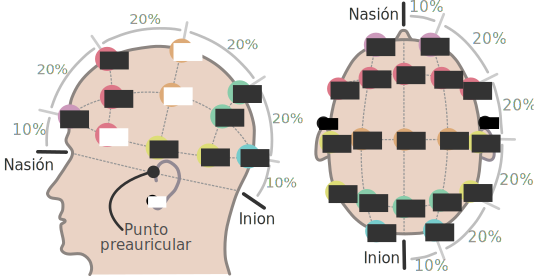
\includegraphics[width=\linewidth]{./img_diagramas/cabeza_proporcionada_color_v4.pdf} 
\caption{Colocación de electrodos según el sistema 10--20}
\label{img1020}
\end{figure}

Debido a que las neuronas en la corteza cerebral tienen orientaciones muy diversas y a que disparan 
de manera asíncrona, además de que el cerebro se encuentra cubierto por las muchas capas descritas
anteriormente, las señales captadas por los electrodos deben ser amplificadas analógicamente antes 
de ser registradas digitalmente.
%
A ello hay que añadir la difusión generada por las meninges, el líquido encefalorraquídeo y el 
cráneo.

Un efecto colateral de amplificar la señal es la inclusión de \textbf{ruido}, entendido como 
señales que son registradas de manera no deseada; como ejemplo, los músculos faciales medianamente 
contraídos generan campos eléctricos con frecuencia de 100 \hz.
%
Este tipo de ruido \textit{persistentes} son eliminados usando un filtro que \textit{elimine} los 
componentes de frecuencia específicos.
%
Los ruidos de duración corta son referidos como \textbf{artefactos}; como ejemplo, pestañear 
voluntariamente durante un episodio de quietud mental interrumpe las ondas alfa por cerca de dos 
segundos. 

Adicionalmente al registro del EEG, la PSG contempla el registro de algunas otras \textit{variables 
fisiológicas} como respiración, ritmo cardíaco, temperatura, entre otros. 
%
En el estudio por Vázquez Tagle y colaboradores, el registro de PSG incluyó registros de actividad 
ocular (\textbf{electrooculograma}, EOG) y tono muscular (\textbf{electromiograma}, EMG), según las 
recomendaciones de la AASM para clasificar las etapas de sueños. La ubicación estos últimos 
electrodos es ilustrada en la figura \ref{emg_eog}.

\begin{figure}
\centering
\includegraphics[width=\linewidth]
{./img_diagramas/emg_eog_v4.pdf}
\caption{Colocación de electrodos para registrar actividad ocular y tono muscular}
\label{emg_eog}
\end{figure}

Para interpretar los registros de EOG (canales LOG, ROG) se puede entender al ojo como una batería
cuyos  polos son la retina y la pupila, y que genera pequeñas variaciones en el campo eléctrico
cuando se mueve; el registro consiste en la proyección del movimiento sobre el eje que forman los
electrodos.
%
Los registros de EMG (canal EMG) admiten una interpretación más \textit{sencilla}, ya que los
músculos son activados directamente por señales eléctricas: el tono muscular es la actividad 
muscular basal, y se relaciona con la velocidad con que los músculos pueden \textit{salir} del 
reposo.

%%%%%%%%%%%%%%%%%%%%%%%%%%%%%%%%%%%%%%%%%%%%%%%%%%%%%%%%%%%%%%%%%%%%%%%%%%%%%%%%%%%%%%%%%%%%%%%%%%%
%%%%%%%%%%%%%%%%%%%%%%%%%%%%%%%%%%%%%%%%%%%%%%%%%%%%%%%%%%%%%%%%%%%%%%%%%%%%%%%%%%%%%%%%%%%%%%%%%%%

\subsection{Estructura del sueño}

Se entiende al sueño como un proceso vital, con una estructura característica, y que en el ser 
humano presenta las siguientes propiedades \cite{CarrilloMora}:
\begin{enumerate}
\item Disminución de conciencia y reactividad a estímulos externos
\item Fácilmente reversible, a diferencia de estados patológicos como estupor y coma
\item Inmovilidad y relajación muscular
\item Periodicidad típica circadiana (diaria)
\item Los individuos adquieren una postura estereotipada
\item La privación induce alteraciones conductuales y 
fisiológicas, además de que genera una \textit{deuda} acumulativa
\end{enumerate}

La duración del sueño es determinada en gran parte por la edad; el recién nacido duerme entre 14 y 
18 horas, el lactante entre 12 y 14 horas, el niño en etapa escolar entre 11 y 12 horas y en la 
edad adulta, la mayoría duerme entre 7 y 8 horas por noche \cite{Contreras13}.
%
Paralelamente el sueño no es un proceso homogéneo, sino que tiene una estructura por etapas con 
rasgos electroencefalográficos y fisiológicos distintivos.

Para su estudio, el sueño se divide en dos etapas: N y R.
%
La \textbf{fase N}, se caracteriza por movimientos oculares lentos, tono muscular que decrece 
constantemente, actividad cerebral que recuerda al reposo, y la presencia de husos de sueño y 
complejos K; en base a ello se divide en las sub-fases N1, N2, N3.

Durante la \textbf{fase R} el tono muscular disminuye (excepto para los músculos respiratorios y 
los esfínteres), la frecuencia cardíaca y respiratoria se vuelve irregular, y el sujeto exhibe 
movimientos oculares rápidos (MOR); en base a lo cual la fase R es conocida como \textbf{sueño 
MOR}.
%
En el EEG, aparecen ondas rápidas de bajo voltaje, irregulares, y que recuerdan la actividad 
durante el estado de alerta; estos patrones no interrumpen el sueño sino que, contrariamente,
incrementan el umbral para estímulos externos, motivo por el cual esta fase también es referida 
como \textbf{sueño paradójico}.
%
Cabe mencionar que durante el sueño MOR se producen la mayoría de las ensoñaciones (referidas 
coloquialmente como \textit{sueños}), y que la mayoría de los pacientes que despiertan durante esta 
fase suelen recordar vívidamente el contenido de sus ensoñaciones \cite{Rosales14}.

\begin{table}
\caption[Criterios para la clasificación de etapas de sueño]
{Criterios para la clasificación de etapas de sueño según la AASM}
\centering
{\small
\begin{tabular}{lllll}
\toprule
&&   & Movimientos & Tono \\
\multicolumn{2}{l}{Etapa}& Características del EEG & oculares & muscular \\
\midrule
Vigilia & W  & {Ritmo alfa} en $>50$\% de la época en   & No & Alto \\
        &    & la región occipital                &    &      \\
NMOR 1  & N1 & Cambio de alfa por AABFM, atenuación & Lentos & $<$W     \\
        &    & del ritmo dominante. Ondas agudas   &    &      \\
NMOR 2  & N2 & Husos de sueño y complejos K en la    & No & $<$W, $>$R     \\
        &    & primera mitad de la época. AABFM &    &     \\
NMOR 3  & N3 & {Ondas lentas} (0.5--2 \hz, $>75$ \mv) en& No & $<$N2, $\approx$R \\
        &    & $>20$\% de la época. Husos de sueño       &&      \\
MOR     & R  & Actividad baja amplitud y frecuencias & MOR's & Bajo  \\
        &    & mixtas. Ondas 'saw-tooth'             &       &       \\
\bottomrule
\multicolumn{4}{l}{Se abrevia AABFM=Actividad de Amplitud Baja y Frecuencias Mixtas}
\end{tabular}\\
}
\end{table}

\begin{figure}
\centering
\includegraphics[width=\linewidth]
{./img_ejemplos/MJNN_epoca_stam.pdf}
\caption[Registro de polisomnograma durante sueño MOR]
{Registro de polisomnograma durante sueño MOR. Marca de calibración: vertical, 10 \mv, horizontal, 
1 segundo}
\label{ejemplos_mor}
\end{figure}

%%%%%%%%%%%%%%%%%%%%%%%%%%%%%%%%%%%%%%%%%%%%%%%%%%%%%%%%%%%%%%%%%%%%%%%%%%%%%%%%%%%%%%%%%%%%%%%%%%%
%%%%%%%%%%%%%%%%%%%%%%%%%%%%%%%%%%%%%%%%%%%%%%%%%%%%%%%%%%%%%%%%%%%%%%%%%%%%%%%%%%%%%%%%%%%%%%%%%%%
%%%%%%%%%%%%%%%%%%%%%%%%%%%%%%%%%%%%%%%%%%%%%%%%%%%%%%%%%%%%%%%%%%%%%%%%%%%%%%%%%%%%%%%%%%%%%%%%%%%

%%%%%%%%%%%%%%%%%%%%%%%%%%%%%%%%%%%%%%%%%%%%%%%%%%%%%%%%%%%%%%%%%%%%%%%%%%%%%%%%%%%%%%%%%%%%%%%%%%%%
%%%%%%%%%%%%%%%%%%%%%%%%%%%%%%%%%%%%%%%%%%%%%%%%%%%%%%%%%%%%%%%%%%%%%%%%%%%%%%%%%%%%%%%%%%%%%%%%%%%
%%%%%%%%%%%%%%%%%%%%%%%%%%%%%%%%%%%%%%%%%%%%%%%%%%%%%%%%%%%%%%%%%%%%%%%%%%%%%%%%%%%%%%%%%%%%%%%%%%%

\chapter{Medida y frecuencia}

Existe una larga tradición para entender y modelar las señales electrofisiológicas en términos de 
\textit{ondas y frecuencias}, ya que fundamentalmente son fenómenos eléctricos \cite{Kaiser00}.
%
Se aborda el enfoque usual del espectro de potencias: se asocia la energía de una señal con su 
dispersión (varianza) y se estudia cómo se distribuye en la base de Fourier.
%
En el entendido de que el espectro de potencias puede variar en el tiempo, la estacionariedad
es equivalente a que el tal cambio no ocurra.

Como el espectro de potencias clásico está definido para funciones, conviene mencionar con las 
definiciones pertinentes sobre procesos estocásticos, y posteriormente deducir condiciones bajo las 
cuales se les puede definir un espectro de potencias.

%%%%%%%%%%%%%%%%%%%%%%%%%%%%%%%%%%%%%%%%%%%%%%%%%%%%%%%%%%%%%%%%%%%%%%%%%%%%%%%%%%%%%%%%%%%%%%%%%%%
%%%%%%%%%%%%%%%%%%%%%%%%%%%%%%%%%%%%%%%%%%%%%%%%%%%%%%%%%%%%%%%%%%%%%%%%%%%%%%%%%%%%%%%%%%%%%%%%%%%

\section{Variables aleatorias}

\begin{definicion}[$\boldsymbol{\sigma}$-álgebra]
Sea $U$ un conjunto y sea $\mathcal{U}$ una colección de subconjuntos de $U$. Se dice que 
$\mathcal{U}$ es una $\sigma$-álgebra si cumple
\begin{itemize}
\item $U \in \mathcal{U}$
\item $A \in \mathcal{U} \Rightarrow A^{C} \in \mathcal{U}$
\item 
$ \displaystyle \{ A_n \}_{n\in \mathbb{N}} \subseteq \mathcal{U} 
\Rightarrow \cup_{n\in \mathbb{N}} A_n \in \mathcal{U}$
\end{itemize}
Donde $A^{C} = \{ u \in U | u \notin A \} $
\end{definicion}

Por simplicidad, sólo se usarán medidas en $\R$ derivadas de $\mathcal{B}$, la $\sigma$-álgebra de 
Borel; ésta se define como la $\sigma$-álgebra más pequeña que contiene a los intervalos abiertos, 
definidos de la manera usual. 

\begin{definicion}[Medida]
Sea $U$ un conjunto y sea $\mathcal{U}$ una $\sigma$-álgebra definida en $U$. Se dice que una 
función $\mu : \mathcal{U} \rightarrow \R_+$ es una medida si cumple que
\begin{itemize}
\item $\mu(\emptyset) = 0$
\item Si $\{ A_n \}_{n\in \mathbb{N}} \subseteq \mathcal{U}$ son tales que 
$A_n \cap A_m = \emptyset \Leftrightarrow m\neq n$, entonces
$$ \mu\left( \bigcup_{n\in \mathbb{N}} A_n \right) = \sum_{n\in \mathbb{N}} \mu(A_n)$$
\end{itemize}
Donde $\R_+ = \{ x\in \R | 0 \leq x \}$ y $\emptyset$ es el conjunto vacío
\label{medida}
\end{definicion}

Una medida de probabilidad en $\R$, $P$, puede verse como una medida definida en $\mathcal{B}$ tal
que $P(\R) = 1$. 
%
Heurísticamente se suele asociar una medida de probabilidad al resultado de un experimento 
\textit{aleatorio}, de modo que el resultado --en este caso, un número-- ocurre dentro de un 
intervalo $I$ con \textit{probabilidad} $100 \times P(I)$.

Para facilitar la interpretación anterior, se define una \textbf{variable aleatoria} (VA) como una 
función $X : U \rightarrow E$ que es medible con respecto a la medida de probabilidad $P$.
%
El conjunto $E$ corresponde a los resultados del experimento que se modela, mientras que $U$ y $P$ 
son como en la definición \ref{medida}.

Una forma de estudiar una VA en $\R$ es a través de su función de probabilidad acumulada (FPA);
esta función da información sobre cómo se \textit{distribuye} la probabilidad, es decir, qué
subconjuntos tienen mayor probabilidad. 
%
En el presente texto únicamente se usarán VA en $\R$.

\begin{definicion}[Función de Probabilidad Acumulada]
Sea $X$ una VA en y sea $P_X$ su medida de probabilidad. Se define su función de 
probabilidad acumulada, $F_X : \R \rightarrow [0,1]$, como
\begin{equation*}
F_X (x) := P\left( \left(-\infty,x \right] \right)
\end{equation*}
\end{definicion}

Si una VA $X$ tiene asociada una FPA que es \textit{absolutamente continua}, entonces se dice que 
$X$ es una \textbf{VA continua}. 
%
El que una FPA sea absolutamente continua es equivalente a que los conjuntos de medida cero en la 
medida de Lebesgue tengan medida cero en la medida de probabilidad asociada a $X$.
%
Adicionalmente en este caso, $F_X$ es derivable y se puede le definir una \textbf{función de 
densidad de probabilidad} (FDA), $f_X$, como $f_X := F_X\prima$.

Se dice que $X$ es una \textbf{VA discreta} si existen $\{ x_n \}_{n\in \mathbb{N}}$ tales que su 
FPA puede escribirse como
%
\begin{equation*}
F_X(x) = \sum_{n \in \mathbb{N}} F_X(x_n^+) - F_X(x_n^-)
\end{equation*}

Conviene destacar que todas la VA poseen una FDP, pero sólo si son continuas poseen una FDA. La
distinción entre VA continuas y discretas puede verse más notoria en virtud del teorema 
\ref{Lebesgue_decomp}.

\begin{teorema}[Descomposición de Radon-Nikodym]
Sea $\mu$ una medida definida sobre la $\sigma$-álgebra $\mathcal{B}$, y sea $\nu$ una medida 
$\sigma$-finita definida sobre $\mathcal{B}$. Entonces $\mu$ puede descomponerse de manera única como
$\mu = \mu_A + \mu_S$, donde
\begin{itemize}
\item $\mu_A$ es absolutamente continua respecto a $\nu$
\item Existe un conjunto $A$ tal que $\nu(A)=0$, $\mu_S\left(A^{C}\right) = 0$
\end{itemize}
\label{Lebesgue_decomp}
\end{teorema}

\begin{definicion}[Medida $\boldsymbol{\sigma}$-finita]
Una medida $\mu$ sobre la $\sigma$-álgebra $\mathcal{U}$, definida para el conjunto $U$, es 
$\sigma$-finita si existen $\{ A_n \}_{n\in \mathbb{N}}$ tales que
\begin{itemize}
\item $\mu\left( A_n \right) < \infty$
\item $\displaystyle \bigcup_{n\in \mathbb{N}} A_n = U$
\end{itemize}
\end{definicion}

La medida de Lebesgue es $\sigma$-finita y entonces cualquier medida de probabilidad puede 
\textit{descomponerse} en una parte continua, una parte discreta y un \textit{residuo}; no hay
garantía de que alguna de ellas resulten ser medidas de probabilidad.

%%%%%%%%%%%%%%%%%%%%%%%%%%%%%%%%%%%%%%%%%%%%%%%%%%%%%%%%%%%%%%%%%%%%%%%%%%%%%%%%%%%%%%%%%%%%%%%%%%%

\section{Estacionariedad débil}

Algunas cantidades asociadas a una variable aleatoria $X$ pueden entenderse en términos de la 
función $\mathrm{E}$ (definición \ref{esperado}), referida como \textit{valor esperado}.
%
Por ejemplo
\begin{itemize}
\item Promedio, $\E{X}$
\item Varianza, $\Var{X} := \E{\left( X - \E{X} \right)^{2}}$
\item Covarianza, $\Cov{X,Y} := \E{\left( X - \E{X} \right)\left( Y - \E{Y} \right)}$
\end{itemize}

\begin{definicion}[Valor esperado]
Sea $X$ una VA cuya FPA es $F_X$ y sea $g: \R \rightarrow \R$ una función arbitraria. El operador
$\mathrm{E}_X$, valore esperado, se define como
\begin{equation}
\mathrm{E}\left[ g(X) \right] := \int_{\R} g(x) dF_X(x)
\end{equation}
La integral está definida en el sentido de Stieltjes
\label{esperado}
\end{definicion}

%%%%%%%%%%%%%%%%%%%%%%%%%%%%%%%%%%%%%%%%%%%%%%%%%%%%%%%%%%%%%%%%%%%%%%%%%%%%%%%%%%%%%%%%%%%%%%%%%%%

Un \textbf{proceso estocástico} \xt es una colección de VA indexadas por el símbolo $t$, referido
como \textbf{tiempo}. El conjunto $\mathcal{T} \subseteq \R$ será referido como \textit{tiempos 
permitidos}, y se tomará como un intervalo cerrado (\textbf{tiempo continuo}) o bien un subconjunto 
de $\left\{ t \in \R | {t} \cdot {\Delta_t} \in \Z \right\} $  para algún $\Delta_t$ 
(\textbf{tiempo discreto}). 
%
Las \textit{componentes} de un proceso estocástico serán denotadas como:\\

\begin{tabular}{cl}
\xt    & Todo el proceso \\
$X(t)$ & Una de las VA que componen al proceso, en el tiempo $t$ \\
$x(t)$ & Una realización de $X(t)$ \\
$F_{X(t)}$ & FPA para $X(t)$ \\
$ {\Delta_t}$ & Frecuencia de muestreo (en tiempo discreto)
\end{tabular}\\

La estacionariedad es un indicativo de la \textit{homogeneidad} de un proceso; un proceso 
\textit{muy} estacionario sería aquél cuyas VA que tiene distribuciones conjuntas que no cambian 
con el tiempo. 
%
La definición \ref{est_fuerte} representa con exactitud tales requerimientos, pero se le considera 
\textit{innecesariamente fuerte}; una definición común es \ref{est_m}.

\begin{definicion}[Estacionariedad fuerte]
Un proceso \xt se dice fuertemente estacionario si para cualesquiera 
$t_1, t_2, \dots, t_n \in \mathcal{T}$ y cualquier $\tau$ tal que $t_i + \tau \in \mathcal{T}$,
se cumple que
\begin{equation*}
F_{\left[ X(t_1), X(t_2), \dots, X(t_n) \right]} \equiv
F_{\left[ X(t_1 + \tau), X(t_2 + \tau), \dots, X(t_n + \tau) \right]}
\end{equation*}
Donde $F_{[v_1,v_2,\dots,v_N]}$ es la FPA conjunta para el vector $[v_1,v_2,\dots,v_N]$
\label{est_fuerte}
\end{definicion}

\begin{definicion}[Estacionariedad de orden $m$]
Un proceso \xt se dice estacionario de orden $m$ si, para cualesquiera
$t_1, t_2, \dots, t_n \in \mathcal{T}$ y cualquier $\tau$ tal que $t_i + \tau \in \mathcal{T}$,
se cumple que
\begin{equation*}
\E{X^{m_1}(t_1)X^{m_2}(t_2)\cdots X^{m_n}(t_n)} =
\E{X^{m_1}(t_1+\tau)X^{m_2}(t_2+\tau)\cdots X^{m_n}(t_n+\tau)}
\end{equation*}
para cualesquiera enteros $m_1, m_2, \dots, m_n$ tales que $m_1+m_2+\cdots+m_n \leq m$
\label{est_m}
\end{definicion}

Cabe mencionar que la definición \ref{est_m} no es equivalente a la definición \ref{est_fuerte}, ni
aún cuando $m\rightarrow \infty$; sin embargo permite asegurar que los \textit{momentos} 
($\E{X^{k}}$ para algún $k$) del proceso sean invariantes en el tiempo, y éstos suelen encontrarse
asociados a cantidades físicas.

Como un ejemplo muy particular conviene destacar la energía, que suele ser asociada con el segundo
momento (definición \ref{energia}). 
%
Dicha conexión motiva a escoger una definición de estacionariedad que permita analizar la energía 
del proceso: la estacionariedad débil.

\begin{definicion}[Estacionariedad débil]
Un proceso \xt se dice débilmente estacionario si existen constantes $\mu, \sigma \in \R$ y una 
función $R : T \rightarrow \R \cup \{ \pm \infty \} $ tales que, para cualesquiera $t, s \in T$ se 
cumple
\begin{itemize}
\item $\E{X(t)} = \mu$
\item $\Var{X(t)} = \sigma^{2}$
\item $\Cov{X(t),X(s)} = R(s-t)$
\end{itemize}
\end{definicion}

\begin{proposicion}
Un proceso es débilmente estacionario si y sólo si es estacionario de orden 2
\end{proposicion}

Cabe destacar que la estacionariedad débil no sólo tiene como condición que todas las variables del
proceso tengan la misma media y varianza, sino que también supone que éstas son finitas.
%
Sobre la función de covarianza $R$ (que en un único proceso es referida como \textit{autocovarianza}),
no hay restricciones sobre los valores que pueda tomar, excepto que 
$R(0) = \Var{X(\bullet)} < \infty$. 
%
En el marco del modelo de series electrofisiológicas, conviene suponer que los registros 
corresponden a procesos a tiempo continuo que son continuos de alguna forma; se ha elegido la 
continuidad en media cuadrática.

%\begin{observacion}
%Sea \xt un proceso débilmente estacionario y $T$ su función de autocovarianza. Si $R$ es continua
%en 0 entonces es continua en todos lados
%\end{observacion}

\begin{definicion}[Continuidad estocástica en media cuadrática]
Un proceso a tiempo continuo \xt es estocásticamente continuo, en el sentido de media cuadrática, 
en un tiempo admisible $t_0$ si
\begin{equation*}
\lim_{t \rightarrow t_0} \E{\left( X(t) - X(t_0) \right)^{2}} = 0
\end{equation*}
\label{cont_est}
\end{definicion}

Una forma natural de pensar en la definición \ref{cont_est} es que si $\abso{t-t_0}$ es muy pequeño 
entonces $X(t)$ y $X(t_0)$ difieren muy poco entre sí, como variables aleatorias.
%
Hablando de procesos débilmente estacionarios, la continuidad estocástica de un proceso es 
equivalente a que su función de autocovarianza sea continua en 0.

%%%%%%%%%%%%%%%%%%%%%%%%%%%%%%%%%%%%%%%%%%%%%%%%%%%%%%%%%%%%%%%%%%%%%%%%%%%%%%%%%%%%%%%%%%%%%%%%%%%
%%%%%%%%%%%%%%%%%%%%%%%%%%%%%%%%%%%%%%%%%%%%%%%%%%%%%%%%%%%%%%%%%%%%%%%%%%%%%%%%%%%%%%%%%%%%%%%%%%%

\section{Transformada de Fourier}

Para exponer formalmente lo que es la transformada de Fourier, conviene mencionar los espacios de 
las \textbf{series $\boldsymbol{p}$-sumables} ($\lp$), y las  \textbf{funciones 
$\boldsymbol{p}$-integrables} sobre un intervalo $I \subseteq \R$ ($\llp_I$).
\begin{align*}
\ell^{p} &:= \left\{ s: \Z\rightarrow\C \talque \sum_{n=-\infty}^{\infty} \abso{s(n)}^{p} < \infty \right\}
\\
L^{p}_I &:= \left\{ S: I\rightarrow\C \talque \int_I \abso{S(t)}^{p} dt < \infty \right\}
\end{align*}

Estos conjuntos admiten las operaciones  suma ($+$), producto ($\cdot$) y multiplicación por 
escalares de la manera usual.
%
Para el caso particular $p=2$, los conjuntos $\ldos$ y $\lldos$ admiten los siguientes productos 
internos:
%
\begin{align*}
\left\langle s,z \right\rangle &= \sum_{n=-\infty}^{\infty} s(n) \overline{z(n)}\\
\left\langle S,Z \right\rangle &= \int_I S(t) \overline{Z(t)} dt
\end{align*}

Usando dichos productos internos, junto con las normas y métricas que inducen, los conjuntos 
$\ldos$ y $\lldos$ tienen estructura de \textit{espacio de Hilbert}.

Las definiciones anteriores revelan cómo $\ldos$ y $\lldos$ son \textit{muy} parecidos, luego
entonces se puede definir la transformada de Fourier como una conexión natural entre ellos.

\begin{definicion}[Serie de Fourier]
Sea $S: \R \rightarrow \C$ una función periódica con periodo $2T$ y tal que 
$S \in L^{2}_{[-T,T]}$. Se dice que $A$ es la serie de Fourier para $S$ si satisface
\begin{equation*}
A(n) = \frac{1}{2 T} \simint{T} S(t) e^{-\nicefrac{ i \abso{n} t}{2T}} dt
\end{equation*}
\label{FourierClasico}
\end{definicion}

\begin{definicion}[Transformada de Fourier]
Sean $S$ y $A$ como en la definición \ref{FourierClasico}. Se le llama transformada de Fourier a la
función $\mathcal{F}_T : L^{2}_{[-T,T]} \rightarrow \ldos : S \mapsto A$
\end{definicion}

Puede interpretarse a $A$ como las \textit{coordenadas} de $S$ en $L^{2}_{[-T,T]}$, usando una base 
de funciones ortonormales $\left\{ e^{\nicefrac{i \abso{n} t}{2 T}} \right\}_{n\in \Z}$; esta base 
en particular es conocida como la \textbf{base de Fourier}.
%
Cabe mencionar las siguientes propiedades de $\mathcal{F}_T$
\begin{itemize}
\item Es lineal, $\mathcal{F}_T[cS + Z] = c\mathcal{F}_T[S] + \mathcal{F}_T[Z]$

\item \textbf{No} es invertible, aunque se le suele definir una pseudoinversa como
\begin{equation*}
\mathcal{F}_{T}^{\text{inv}} : \ldos \rightarrow L^{2}_{[-T,T]} :
A \mapsto \sum_{n -\infty}^{\infty} A(n) e^{\nicefrac{i \abso{n} t}{2 T}}
\end{equation*}
\end{itemize}

Se define, de manera pragmática, la \textbf{energía disipada} y la \textbf{potencia} de una función 
$S$ en un intervalo $[a,b]$ como 
\begin{align}
\text{energía}[S]_{[a,b]} &= \int_a^{b} \abso{S(t)}^{2} dt \nonumber \\
\text{potencia}[S]_{[a,b]} &= \frac{1}{b-a} \int_a^{b} \abso{S(t)}^{2} dt
\label{energia}
\end{align}

Es evidente que la energía y potencia están relacionadas a la norma en $L^{2}_{[-T,T]}$ inducida por
su producto interno.
%
Dicha relación junto a las propiedades \textit{agradables} de $\mathcal{F}_T$ pueden ser usadas 
para conectar la energía con la norma en $\ldos$ (teorema \ref{parseval}): la energía disipada por 
una función equivale a la suma de las energías disipada por cada una de sus \textit{componentes} en 
la base de Fourier.
%
Conviene, entonces, definir una función que \textit{desglose} estos \textit{aportes}.

\begin{teorema}[Parseval]
Sea $S \in L^{2}_{[-T,T]}$, y sea $A = \mathcal{F}[S]$. Se cumple que
\begin{equation*}
\int_{-T}^{T} \abso{S(t)}^{2} dt = \sum_{n=-\infty}^{\infty} \abso{A(n)}^{2}
\end{equation*}
\label{parseval}
\end{teorema}

\begin{definicion}[Espectro de potencias]
Sea $S \in L^{2}_{[-T,T]}$, y sea $A = \mathcal{F}[S]$. Se llama espectro de potencias 
para $S$ a la función $h_S : \R \rightarrow \R $, definida como
\begin{equation*}
h_S(\omega) = 
\begin{cases}
\abso{A(n)}^{2} & \text{ , si } \omega = \nicefrac{n}{2T}, \text{   con } n\in \mathbb{Z} \\
0 & \text{ ,  otro caso}
\end{cases}
\end{equation*}
\label{espec}
\end{definicion}

Un elemento que será de crucial importancia en el desarrollo posterior es la \textbf{convolución} 
($\ast$), una tercera operación binaria en estos espacios y definida como
%
\begin{align*}
[s \ast z] (\tau) &= \sum_{n=-\infty}^{\infty} s(n) \overline{z(\tau-n)} \\
[S \ast Z] (\tau) &= \int_I S(t) \overline{Z(\tau-t)}
\end{align*}
%
donde $\overline{c}$ es el conjugado complejo de $c$. 
%
Esta operación cobra importancia por la forma en que se relaciona con $\mathcal{F}_T$
%
\begin{observacion}%[de la convolución]
Sean $S,Z \in L^{2}_{[-T,T]}$, entonces se satisface que
\begin{align*}
\mathcal{F}_T[S\ast Z]  &= \mathcal{F}_T[S] \cdot \mathcal{F}_T[Z] \\
\mathcal{F}_T[S\cdot Z] &= \mathcal{F}_T[S] \ast  \mathcal{F}_T[Z] 
\end{align*}
\label{t_convolucion}
\end{observacion}

%%%%%%%%%%%%%%%%%%%%%%%%%%%%%%%%%%%%%%%%%%%%%%%%%%%%%%%%%%%%%%%%%%%%%%%%%%%%%%%%%%%%%%%%%%%%%%%%%%%
%%%%%%%%%%%%%%%%%%%%%%%%%%%%%%%%%%%%%%%%%%%%%%%%%%%%%%%%%%%%%%%%%%%%%%%%%%%%%%%%%%%%%%%%%%%%%%%%%%%

\section{Función de densidad espectral}

La forma más natural de definir un espectro de potencias para un proceso estacionario es a través 
de la tr. de Fourier de sus realizaciones. En general no se puede garantizar que una definición así \textit{funcione} ya que las realizaciones pueden ser señales que no son periódicas, 
cuadrado-integrable, continuas, etc.
%
Este problema será abordado al restringir los tiempos permitidos a un conjunto \textit{sin 
problemas}, para luego considerar el límite cuando \textit{recupera su forma original}.

\begin{definicion}[Función de densidad espectral, tiempo continuo]
Sea \xt un proceso estacionario a tiempo continuo. Se define su {función de densidad 
espectral} como
\begin{equation}
h(\omega) = \frac{1}{2 \pi} \lim_{T\rightarrow \infty} \E{ \frac{1}{2T} 
\abso{ \int_{-T}^{T} X(t) e^{-i \omega t} dt}^{2} }
\label{txt_FDE_cont}
\end{equation}
\end{definicion}

\begin{definicion}[Función de densidad espectral, tiempo discreto]
Sea $\{X(t)\}_{\nicefrac{t}{\Delta_t}\in \Z}$ un proceso estacionario a tiempo discreto. Se 
define su {función de densidad espectral} como
\begin{equation}
h(\omega) = \frac{1}{2 \pi} \lim_{N\rightarrow \infty} \E{ \frac{1}{2N} 
\abso{ \sum_{n=-N}^{N} X(n \Delta_t) e^{-i \omega n \Delta_t}}^{2} }
\label{txt_FDE_disc}
\end{equation}
\end{definicion}

De la defunción se deduce que la función de densidad espectral (FDE) siempre es una función
no-negativa

%%%%%%%%%%%%%%%%%%%%%%%%%%%%%%%%%%%%%%%%%%%%%%%%%%%%%%%%%%%%%%%%%%%%%%%%%%%%%%%%%%%%%%%%%%%%%%%%%%%
%%%%%%%%%%%%%%%%%%%%%%%%%%%%%%%%%%%%%%%%%%%%%%%%%%%%%%%%%%%%%%%%%%%%%%%%%%%%%%%%%%%%%%%%%%%%%%%%%%%

%\section{Representación espectral}

\begin{teorema}[Wiener-Khinchin]
Una condición suficiente y necesaria para que $\rho$ sea una función de autocorrelación de 
algún proceso estocástico a tiempo continuo $\{X(t)\}$ débilmente estacionario y 
estocásticamente continuo, es que exista una función $F$ que tenga las siguientes propiedades
\begin{itemize}
\item Monótonamente creciente
\item $F(-\infty) = 0$
\item $F(+\infty) = 1$
\end{itemize}
y tal que para todo $\tau \in \R$ se cumple que
\begin{equation*}
\rho(\tau) = \intR e^{i \omega \tau} dF(\omega)
\end{equation*}
\label{t_wienerkhinchin}
\end{teorema}

\begin{teorema}[Wold]
Una condición suficiente y necesaria para que $\rho$ sea una función de autocorrelación de 
algún proceso estocástico a tiempo discreto $\{X(t)\}$ débilmente estacionario es que exista 
una función $F$ con las siguientes propiedades
\begin{itemize}
\item Monótonamente creciente
\item $F(-\pi) = 0$
\item $F(+\pi) = 1$
\end{itemize}
y tal que para todo $\tau \in \R$ se cumple que
\begin{equation*}
\rho(\tau) = \intPI e^{i \omega \tau} dF(\omega)
\end{equation*}
\label{t_wold}
\end{teorema}

\begin{teorema}
Sea \xt un proceso a tiempo continuo, débilmente estacionario, de media 0 y estocásticamente 
continuo en el sentido de media cuadrática. Entonces, existe un proceso 
ortogonal $\{Z(\omega)\}$ tal que, para todo tiempo $\omega$ admisible, se puede 
escribir
\begin{equation*}
X(t) = \intR e^{i t \omega} dZ(\omega)
\end{equation*}
Donde el proceso $\{Z(t)\}$ tiene las siguientes propiedades para todo $\omega$
\begin{itemize}
\item $\E{dZ(\omega)} = 0$
\item $\E{\abso{dZ(\omega)}^{2}} = dH(\omega)$
\item $\Cov{dZ(\omega),dZ(\lambda)} = 0 \Leftrightarrow \omega \neq \lambda$
\end{itemize}
Donde $dH(\omega)$ la FDE integrada de $\{X(t)\}$
\label{rep_espectral}
\end{teorema}

En virtud del teorema de Wold, se puede tener una variante del teorema de Wiener-Khinchin
para procesos a tiempo discreto, razón por la cual  
tal representación es referida como \textbf{representación de Wold-Cramér}.

%%%%%%%%%%%%%%%%%%%%%%%%%%%%%%%%%%%%%%%%%%%%%%%%%%%%%%%%%%%%%%%%%%%%%%%%%%%%%%%%%%%%%%%%%%%%%%%%%%%
%%%%%%%%%%%%%%%%%%%%%%%%%%%%%%%%%%%%%%%%%%%%%%%%%%%%%%%%%%%%%%%%%%%%%%%%%%%%%%%%%%%%%%%%%%%%%%%%%%%

\subsection{Unidades de tiempo y efecto \textit{alias}}

Merecen especial atención los procesos a tiempo discreto que son generados al registrar 
digitalmente procesos a tiempo continuo, procedimiento referido como \textit{muestreo}.
%
Dicho procedimiento está limitado por la velocidad con que se pueden registrar mediciones, así 
como por la capacidad para almacenar los datos obtenidos; tales limitaciones deben tomarse en 
cuenta dentro del diseño experimental para el fenómeno que se estudia, pero no se discutirán aquí.

Sobre el efecto del muestreo, considérese un proceso a tiempo continuo y débilmente estacionario, 
\xt, y sea $\Delta_t \in \R$ arbitrario.
%
Se construye al proceso $\{Y(n)\}_{n\in \mathbb{N}}$ como
\begin{equation}
Y(n) = X(n \Delta_t)
\end{equation}

En virtud del teorema \ref{rep_espectral}, \xt admite una representación de la forma
\begin{equation}
X(t) = \intR e^{i \omega t }  dZ_X(\omega)
\end{equation}

Luego entonces puede reescribirse
\begin{align}
Y(n) &= \intR e^{i \omega n \Delta_t} dZ_X(\omega) \nonumber \\
&= \sum_{k \in \N} \int_{\nicefrac{(2k-1)\pi}{\Delta_t}}^{\nicefrac{(2k+1)\pi}{\Delta_t}}
e^{i \omega n \Delta_t} dZ_X(\omega) \nonumber \\
&= \sum_{k \in \N} \int_{-\nicefrac{\pi}{\Delta_t}}^{\nicefrac{\pi}{\Delta_t}}
e^{i \left( \omega + \frac{2 k \pi}{\Delta_t} \right) n \Delta_t}
dZ_X\left( \omega + \nicefrac{2 k \pi}{\Delta_t}\right) \nonumber \\
&= \sum_{k \in \N} \int_{-\nicefrac{\pi}{\Delta_t}}^{\nicefrac{\pi}{\Delta_t}}
e^{i \omega n \Delta_t}
dZ_X\left( \omega + \nicefrac{2 k \pi}{\Delta_t}\right)
\end{align}

Con base a lo anterior, puede definirse para 
$\omega \in \left[ -\nicefrac{\pi}{\Delta_t} , \nicefrac{\pi}{\Delta_t} \right]$
\begin{equation}
dZ_Y(\omega) := \sum_{k \in \N} dZ_X\left( \omega + \nicefrac{2 k \pi}{\Delta_t}\right)
\end{equation}

En base al teorema \ref{rep_espectral}, se define para 
$\abso{\omega} \leq \nicefrac{\pi}{\Delta_t}$
\begin{align}
dH_Y(\omega) &= \E{\abso{dZ_Y(\omega)}^{2}} \nonumber \\
&= \E{\abso{\sum_{k \in \N} dZ_X\left( \omega + \nicefrac{2 k \pi}{\Delta_t}\right)}^{2}}
\nonumber \\
&= \sum_{k \in \N} \E{\abso{dZ_X\left( \omega + \nicefrac{2 k \pi}{\Delta_t}\right)}^{2}}
\nonumber \\
&= \sum_{k \in \N} dH_X\left( \omega + \nicefrac{2 k \pi}{\Delta_t}\right)
\end{align}

En el segundo paso se usa que $\{ dZ_X \}$ es un proceso ortogonal de media cero.
Antes de poder declara que $dH_Y$ es el espectro integrado del proceso discretizado,
conviene hacer el cambio de variable $\wdd := \omega \Delta_t$
\begin{align*}
dH_Y(\wdd) &= dH_Y(\omega \Delta_t) \frac{d\wdd}{d\omega} \\
&= \frac{1}{\Delta_t} dH_Y(\omega \Delta_t)
\end{align*}
donde $\abso{\wdd} \leq \pi$.
%
Si \xt posee un espectro puramente continuo --de manera equivalentemente, si $dH_X$ es 
absolutamente continua-- entonces puede escribirse
\begin{equation}
h_Y(\wdd) = \frac{1}{\Delta_t} \sum_{k \in \N} h_X\left( \omega + \nicefrac{2 k \pi}{\Delta_t}\right)
\end{equation}
con $\abso{\omega} \leq \pi$. 
%
Así entonces $h_Y$ puede entenderse como una versión \textit{colapsada} de $h_X$, fenómeno conocido 
como \textbf{efecto alias}.

%%%%%%%%%%%%%%%%%%%%%%%%%%%%%%%%%%%%%%%%%%%%%%%%%%%%%%%%%%%%%%%%%%%%%%%%%%%%%%%%%%%%%%%%%%%%%%%%%%%

\subsection{Filtros lineales}

Otra familia de procesos que merecen atención especial son aquellos de la forma son aquellos 
construidos de la forma
\begin{equation}
Y(t) = \intR g(u) X(t-u) du
\end{equation}
%
con \xt un proceso a tiempo continuo, débilmente estacionario, y $g\in L^{2}_{\R}$ una función 
simétrica, por simplicidad. 
%
La conexión entre las FDE respectivas puede obtenerse escribiendo
\begin{align*}
X(t) &= \intR e^{i \omega t }  dZ_X(\omega) \\
Y(t) &= \intR g(u) \left[ \intR e^{i \omega (t-u) }  dZ_X(\omega) \right] du \\
&= \intR e^{i \omega t } \left[ \intR g(u) e^{i \omega -u } du \right] dZ_X(\omega) \\
&= \intR e^{i \omega t } \Gamma(\omega) dZ_X(\omega)
\end{align*}
donde $\Gamma(\omega) = \intR g(u) e^{i \omega -u } du$. 
%
Luego entonces
\begin{align*}
dH_Y(\omega) &= \E{\abso{dZ_Y(\omega)}^{2}}  \\
&= \E{\abso{\Gamma(\omega) dZ_X(\omega)}^{2}}  \\
&= \abso{\Gamma(\omega)}^{2} dH_X(\omega)
\end{align*}

Se concluye que si ambos procesos tengan FDE bien definidas, se cumple que
\begin{equation}
h_Y(\omega) = \abso{\Gamma(\omega)}^{2} h_X(\omega)
\end{equation}
%
lo cual se esperaba heurísticamente como generalización de la relación entre convolución y tr. de
Fourier.

Como notación la función $g$ será referida como \textbf{función de respuesta}, mientras que 
$\Gamma$ es la \textbf{función de transferencia}. 
%
Estos nombre nacen de la interpretación de $Y$ como el resultado de \textit{pasar} a $X$ a través 
de un circuito RC:
si $X$ no fuera un un \textit{pulso} unitario de longitud infinitesimal entonces $Y$ sería $g$,
y si $X$ fuera una función periódica entonces $Y$ sería un pulso unitario.

Conviene destacar que el papel de los filtros se ve incrementando en dos casos particuares:
\begin{itemize}
\item En la interpretación como circuito RC, si $\Gamma$ fuera 1 sobre un intervalo de frecuencias
y 0 en otro caso entonces puede decirse que el sistema \textit{filtra} dichas frecuencias.
%
Estos objetos son físicamente posibles de manera aproximada, y son de uso común 
en el procesamiento de señales para eliminar algunos artefactos
\item Considérese una versión más general de $Y$ como
\begin{equation}
Y(t) = \intR X(t-u) dG(u)
\end{equation}
con $G$ absolutamente continua. Entonces es posible generalizar la teoría de filtros para incluir
al operador de retraso, definido como $B_{\Delta_t}[Y](t) = Y(t-\Delta_t)$, y con ello se pueden
establecer equivalencias con los métodos basados en modelos tipo ARIMA
\end{itemize}
Por simplicidad, ninguno de estos enfoques será explorado en el presente trabajo.

%%%%%%%%%%%%%%%%%%%%%%%%%%%%%%%%%%%%%%%%%%%%%%%%%%%%%%%%%%%%%%%%%%%%%%%%%%%%%%%%%%%%%%%%%%%%%%%%%%%
%%%%%%%%%%%%%%%%%%%%%%%%%%%%%%%%%%%%%%%%%%%%%%%%%%%%%%%%%%%%%%%%%%%%%%%%%%%%%%%%%%%%%%%%%%%%%%%%%%%

\section{Estimadores}

Sea \xt un proceso débilmente estacionario cuyo espectro es puramente continuo, y \xtd un registro 
de una realización, de tamo $N$. 
%
El objetivo de esta sección es calcular la FDE del proceso a partir del registro obtenido.
%
Con vista en la expresión \ref{txt_FDE_disc}, un estimador natural es el \textbf{periodograma}, 
definido como
\begin{equation}
I_N(\omega) = \frac{1}{N} \abso{\sum_{t = 0}^{N} e^{i \omega t} x(t)}^{2}
\label{txt_periodograma}
\end{equation}

%Para poder estudiar mejor al periodograma conviene escribirlo como
%\begin{align*}
%I_N(\omega) &= \frac{1}{N} \abso{\sum_{t = 0}^{N} e^{i \omega t} x(t)}^{2} \\
%&= \frac{1}{N} \left( \sum_{t = 0}^{N} e^{i \omega t} x(t) \right)
%\overline{ \left( \sum_{t = 0}^{N} e^{i \omega t} x(t) \right) } \\
%&= \frac{1}{N} \left( \sum_{t = 0}^{N} e^{i \omega t} x(t) \right)
%\left( \sum_{t = 0}^{N} e^{-i \omega t} x(t) \right) \\
%&= \frac{1}{N} \sum_{n = 0}^{N}
%x(n)^{2} \\
%&\phantom{=}
%+ \frac{1}{N} \sum_{\tau = -N}^{-1} \sum_{n = 0}^{N+\tau}
%x(n)x(n-\tau) e^{i \omega \tau} \\
%&\phantom{=}
%+ \frac{1}{N} \sum_{\tau = 1}^{N} \sum_{n = \tau}^{N}
%x(n)x(n-\tau) e^{i \omega \tau} \\
%\end{align*}

Se puede demostrar que $\E{I_N(\omega)} = h(\omega)$, de modo que es un estimador 
\textbf{insesgado}. Sin embargo, también se demuestra que
\begin{equation*}
\lim_{N\rightarrow \infty} \Var{I_N(\omega)} = \left( h(\omega) \right)^{2}
\end{equation*}
de modo que es un estimador \textbf{inconsistente}, lo cual lo descalifica para usarse en la 
práctica.
%
Para entender por qué el periodograma es inconsistente, conviene escribirlo como
\begin{equation}
I_N(\omega) = 2 \sum_{\tau = -(N-1)}^{N-1} \widehat{R}^{\star}(\tau) \COS{\omega \tau}
\label{txt_periodograma2}
\end{equation}
%
donde $\widehat{R}^{\star}$ es un estimador para la función de autocovarianza, $R$, definido como
\begin{equation}
\widehat{R}^{\star} (\tau) = \frac{1}{N} \sum_{t = 1}^{N-\abso{\tau}} x(t) x(t+\abso{\tau})
\end{equation}

%Se puede demostrar que $\widehat{R}^{\star}$ es consistente y \textit{asintóticamente insesgado}.
%
La expresión \ref{txt_periodograma2} bien puede verse como una inversión de la relación entre la
FDE y la autocovarianza dada por el teorema \ref{t_wold}.
%
Así mismo, la misma expresión puede interpretarse como que el periodograma es una suma ponderada de 
los valores de $\widehat{R}^{\star}$; mientras más grande es $\tau$, menos parejas de puntos cuya 
distancia es $\tau$, y entonces $\widehat{R}^{\star}$ tiene mayor varianza cuanto mayor sea $\tau$. 

Dado que la inconsistencia del periodograma es porque el periodograma es construido usando 
estimadores con varianza elevada, la solución natural es evitar tales componentes. Para ello, 
escójase una función de pesos, $g: \R \rightarrow \R$, defínase
%
\begin{equation}
\widehat{h}(\omega) = \frac{1}{2 \pi} \sum_{\tau = -(N-1)}^{N-1} g(\tau) \widehat{R}^{\star}(\tau) 
e^{i \omega \tau} 
\label{txt_estimador}
\end{equation}

Resulta ilustrativo reescribir a $\widehat{h}$ en términos del periodograma
\begin{equation*}
\widehat{h}(\omega) = \frac{1}{2 \pi} \intPI I_N(\theta) \Gamma(\omega - \theta) d\theta
\end{equation*}
donde $\Gamma(\omega) = \intR g(u) e^{i \omega -u } du$.
%
Se puede demostrar que este tipo de estimadores son asintóticamente insesgado y consistentes.

%%%%%%%%%%%%%%%%%%%%%%%%%%%%%%%%%%%%%%%%%%%%%%%%%%%%%%%%%%%%%%%%%%%%%%%%%%%%%%%%%%%%%%%%%%%%%%%%%%%
%%%%%%%%%%%%%%%%%%%%%%%%%%%%%%%%%%%%%%%%%%%%%%%%%%%%%%%%%%%%%%%%%%%%%%%%%%%%%%%%%%%%%%%%%%%%%%%%%%%
%%%%%%%%%%%%%%%%%%%%%%%%%%%%%%%%%%%%%%%%%%%%%%%%%%%%%%%%%%%%%%%%%%%%%%%%%%%%%%%%%%%%%%%%%%%%%%%%%%%
%%%%%%%%%%%%%%%%%%%%%%%%%%%%%%%%%%%%%%%%%%%%%%%%%%%%%%%%%%%%%%%%%%%%%%%%%%%%%%%%%%%%%%%%%%%%%%%%%%%

\chapter{Espectro evolutivo}

\begin{proposicion}
Sean $u$ y $v$ dos funciones con las siguientes características
\begin{itemize}
\item $\argmax_x u(x), \argmax_x u(x) \ni 0$
\item $\intR \abso{u(x)} dx, \intR \abso{v(x)} dx < \infty$
\item $\intR x\abso{u(x)} dx, \intR x\abso{v(x)} dx < \infty$
\end{itemize} 
Si además se satisface que $u$ tiene una {concentración} muy alta con relación a $v$
($ \intR \abso{u(x)} dx << \intR \abso{v(x)} dx $),
entonces se cumple que
\begin{equation*}
\intR u(x) v(x+k) dx \approx v(k) \intR u(x) dx
\end{equation*}
\label{pseudo_d}
\end{proposicion}

%En el presente trabajo se ha elegido usar el espectro evolutivo, propuesto por Priesltley en
%1965 \cite{Priestley65} debido a que fue diseñado específicamente para (1) conservar linealidad 
%(2) ser siempre positivo, (3) conservar la interpretación física como distribución de energía
%\cite{Loynes68}.

%%%%%%%%%%%%%%%%%%%%%%%%%%%%%%%%%%%%%%%%%%%%%%%%%%%%%%%%%%%%%%%%%%%%%%%%%%%%%%%%%%%%%%%%%%%%%%%%%%%
%%%%%%%%%%%%%%%%%%%%%%%%%%%%%%%%%%%%%%%%%%%%%%%%%%%%%%%%%%%%%%%%%%%%%%%%%%%%%%%%%%%%%%%%%%%%%%%%%%%

%\section{Estimación del espectro evolutivo}

%Una vez definido el espectro evolutivo para procesos no-estacionarios con varianza finita, cabe 
%preguntarse sobre le estimación de esta cantidad a partir de una realización del proceso usando, 
%por ejemplo, periodogramas modificados; tal pregunta no tiene, en general, una respuesta 
%satisfactoria.
%Es por ello que se define una colección, más restringida, de procesos no-estacionarios cuyo 
%espectro evolutivo pueda ser estimado efectivamente usando la técnica de ventanas.

Considerando un proceso no-estacionario \xt que admite una representación de la forma 
$X(t) = \intR A(t,\omega) e^{i \omega t} dZ(\omega)$, entonces el espectro evolutivo queda definido 
como
\begin{equation}
dF_t(\omega) = \abso{A(t,\omega)}^{2} d\mu(\omega)
\label{esp_evolutivo}
\end{equation}

Antes de poder usar la proposición \ref{pseudo_d} para estimar $F_t$ (con respecto a $t$) usando 
una ventana espectral, hay que medir la dispersión de $F_t$ en el tiempo; más aún, hay que pedir 
que esa dispersión sea finita.
Con vista a la ecuación \ref{esp_evolutivo}, se puede usar la conexión entre $F$ y $A$ para 
establecer condiciones respecto a la segunda; se define entonces a $H_\omega$, la transformada de
Fourier de $A$ en el tiempo
\begin{equation}
A(t,\omega) = \intR e^{i t \theta} dH_\omega(\theta)
\end{equation}

Posteriormente se define a $B_{\mathbf{F}}$, el ancho de banda para $H_\omega$ con respecto a la 
familia de funciones $\mathbf{F}$, como
%
\begin{equation}
B_{\mathbf{F}}(\omega) = \intR \abso{\theta} \abso{dH_\omega(\theta)}
\end{equation}

Se dice que el proceso es semi-estacionario con respecto a $\mathbf{F}$ si 
$\sup_\omega B_{\mathbf{F}} < \infty$. El proceso se dice simplemente \textbf{semi-estacionario} 
si esta cantidad es acotada para cualquier familia de funciones admisibles 
$\mathbf{F} \in \mathbf{C}$; entonces se puede definir la constante $B_X$, el \textit{ancho de 
banda característico de} \xt, como

\begin{equation}
B_X = \sup_{\mathbf{F}\in \mathbf{C}} \left[ \sup_\omega B_{\mathbf{F}}(\omega) \right]^{-1}
\end{equation}

la cual será importante como cota para estimar efectivamente el proceso.

%%%%%%%%%%%%%%%%%%%%%%%%%%%%%%%%%%%%%%%%%%%%%%%%%%%%%%%%%%%%%%%%%%%%%%%%%%%%%%%%%%%%%%%%%%%%%%%%%%%
%%%%%%%%%%%%%%%%%%%%%%%%%%%%%%%%%%%%%%%%%%%%%%%%%%%%%%%%%%%%%%%%%%%%%%%%%%%%%%%%%%%%%%%%%%%%%%%%%%%

\section{Estimador de doble ventana}

Respecto a la estimación del espectro local se usa el \textbf{estimador de doble ventana}, 
técnica introducida por Priestley \cite{Priestley69} y que requiere dos funciones, $w_\tau$ y 
$g_\kappa$, que funcionan como ventana de retrasos y como filtro lineal, respectivamente.
%
En cuando a $g_\kappa$, se define a $\Gamma_\kappa(u) = \intR g(u) e^{i u \omega} du$ y se les pide que
\begin{equation*}
2\pi \int_{-\infty}^{\infty} \lvert g_\kappa(u) \lvert^{2} du 
= 
\int_{-\infty}^{\infty} \lvert \Gamma_\kappa(\omega) \lvert^{2} d\omega
= 1
\end{equation*}

Posteriormente se define el estimador $U$ con el objetivo de asignar pesos en el tiempo para estimar
a la FDE
\begin{equation*}
U(t,\omega) = \int_{t-T}^{t} g_\kappa(u) X({t-u}) e^{i \omega (t-u)} du
\end{equation*}

Una vez definida la cantidad $B_X$, y habiendo supuesto que no es 0, es demostrado en 
\cite{Priestley65} que el estimador $U$ satisface que
%
\begin{equation}
\E{\abso{U(t,\omega)}^{2}} = \intR \abso{\Gamma(\omega)}^{2} h(t,\omega+\omega_0) d\omega
+ \orden\left( \nicefrac{B_g}{B_X} \right)
\end{equation}

Bajo el entendido que la función $\Gamma_\kappa$ converge a una función tipo \dirac, puede 
considerarse que 
$\E{\abso{U(t,\omega)}^{2}} \approx h(t,\omega)$; sin embargo, se demuestra en \cite{Priestley66} 
que $\Var{\abso{U(t,\omega)}^{2}} \nrightarrow 0$.
%
Debido a ello se usa una segunda función tipo ventana,
de forma similar al periodograma.
Se considera la función $W_\tau$, ventana de retrasos, y su respectiva ventana espectral 
$w_\tau$; deben satisfacer las siguientes propiedades:
\begin{itemize}
\item $w_{\tau}(t) \geq 0$ para cualesquiera $t$, $\tau$
\item $w_{\tau}(t) \rightarrow 0$ cuando $\lvert t \lvert \rightarrow \infty$, para todo $\tau$
\item $\displaystyle \int_{-\infty}^{\infty} w_{\tau}(t) dt = 1$ para todo $\tau$
\item $\displaystyle \int_{-\infty}^{\infty} \left( w_{\tau}(t) \right)^{2} dt < \infty$ para todo $\tau$
\item $\exists C$ tal que  
$\displaystyle \lim_{\tau\rightarrow\infty} \tau \int_{-\infty}^{t} \abso{ W_{\tau}(\lambda) }^{2} d\lambda = C$
\end{itemize}

Finalmente, se define el estimador $\est{h}$ para las FDE normalizada, $h$, como
\begin{equation*}
\widehat{h}(t,\omega) = \int_{t-T}^{t} w_{\tau}(u) \lvert U(t-u,\omega) \lvert^{2} du
\label{estimador_doble_ventana}
\end{equation*}

Fue demostrado por Priestley \cite{Priestley65} que los estimadores de doble ventana son 
asintóticamente insesgados y consistentes, y propone las siguientes aproximaciones:
\begin{itemize}
\item $\displaystyle
\E{\est{h}(t,\omega)} \approx 
\intR \widetilde{h}(t,\omega+\theta) \abso{\Gamma_\kappa(\theta)}^{2} d\theta$
\item $\displaystyle
\Var{\est{h}(t,\omega)} \approx \frac{C}{\tau} \left( \overline{h}^{2}(\omega) \right)
\intR \abso{\Gamma_\kappa(\theta)}^{4} d\theta $
\end{itemize}

donde las funciones $\widetilde{h}$ y $\overline{h}$ son versiones \textit{suavizadas} de la FDE 
normalizada, $h$, y están definidas de la siguiente manera
\begin{equation*}
\widetilde{h}(t,\omega+\theta) = 
\intR W_{\tau}(u) h(t-u,\omega+\theta) du
\end{equation*}
\begin{equation*}
\overline{h}^{2} (t,\omega) =
\frac{\intR h^{2}\left(t-u,W_{\tau}^{2}(u)\right) du}
{\intR \left( W_{\tau}(u) \right)^{2} du}
\end{equation*}

Como $W_{\tau}$ funciona como ventana espectral, converge a una 
función tipo \dirac; luego $\widetilde{h}$ es aproximadamente la convolución 
$\widetilde{h}(t,\omega+\theta) \approx \delta_t \ast h(\bullet,\omega+\theta)$. 
Una aproximación muy similar 
puede hacerse respecto al segundo término, de modo que $\widetilde{h}\approx h$ y 
$\overline{h}^{2}\approx h^{2}$.
Tales aproximaciones serán mejores en tanto las ventanas $w_{\tau}$ y $W_{\tau}$ sean más 
cercanas a funciones tipo \dirac.
Dicho esto, se pueden hacer las siguientes aproximaciones, un poco más arriesgadas:
\begin{itemize}
\item $\displaystyle \E{\est{h}(t,\omega)} \approx h(t,\omega)$
\item $\displaystyle \Var{\est{h}(t,\omega)} \approx 
\frac{C}{\tau} h^{2}(t,\omega) \intR \abso{\Gamma_\kappa (\theta)}^{4} d\theta$
\end{itemize}

%%%%%%%%%%%%%%%%%%%%%%%%%%%%%%%%%%%%%%%%%%%%%%%%%%%%%%%%%%%%%%%%%%%%%%%%%%%%%%%%%%%%%%%%%%%%%%%%%%%
%%%%%%%%%%%%%%%%%%%%%%%%%%%%%%%%%%%%%%%%%%%%%%%%%%%%%%%%%%%%%%%%%%%%%%%%%%%%%%%%%%%%%%%%%%%%%%%%%%%

\section{Prueba de Priestley-Subba Rao}

La prueba de estacionariedad propuesta por Priestley y Subba Rao \cite{Priestley69} consiste en 
probar la hipótesis de que el espectro evolutivo efectivamente cambia en el tiempo. 
%
El proceso consiste en \textit{calcular} el logaritmo del espectro evolutivo para algunos tiempos y 
frecuencias puntuales, para lo cual se usa el estimador de doble ventana, y posteriormente usar un
análisis ANOVA para verificar si dichas cantidades tienen el mismo valor esperado --recordando que
el estimador de doble ventana es asintóticamente consistente.

Sea \xt un proceso semi-estacionario y sea \xtd un conjunto de observacion, cuya frecuencia de 
muestreo es $\Delta_t=1$ por simplicidad.
%
Usando estos datos se construye el estimador de doble ventana, $\widehat{h}$; para ello se eligen 
como parámetros las funciones $g_\kappa$ y $w_\tau$, que dependen a su vez de los parámetros 
$\kappa$ y $\tau$, y por consecuencia a sus respectivas tr. de Fourier $\Gamma_\kappa$ y $W_\tau$.
%
Bajo las condiciones descritas en la sección anterior, se satisface que
%
\begin{align*}
\E{\widehat{h}(t,\omega)} &\approx h(t,\omega) \\
\Var{\widehat{h}(t,\omega)} &\approx 
\frac{C}{N} h^{2}(t,\omega) \intR \abso{\Gamma^{4}(\theta)} d\theta
\end{align*}
%
donde $\displaystyle C = \lim_{T\rightarrow \infty} T \intR \abso{W_T(\lambda)} d\lambda$.
%
Como es habitual en el estudio del espectro de potencias, se propone la cantidad 
\begin{equation}
Y(t,\omega) = \log\left(\widehat{h}(t,\omega)\right)
\end{equation}
que, por ser $\log$ una función inversible y derivable, cumple que
%
\begin{align*}
\E{Y(t,\omega)} &\approx \log\left(h(t,\omega)\right) \\
\Var{Y(t,\omega)} &\approx 
\frac{C}{T} \intR \abso{\Gamma_\kappa(\theta)}^{4} d\theta \\
\end{align*}

Cabe destacar que la varianza de $Y$ no es independiente de $h$ en el sentido formal, sino que 
sólo es \textit{aproximadamente independiente} pues depende en mayor medida de la forma de 
$\widehat{h}$ que del mismo $h$.
%
Esto era de esperarse, ya que el estimador de doble ventana fue diseñado para exagerar el 
\textit{peso} de la información local. 
%
En otra dirección, la independencia aproximada sugiere que $Y$ puede escribirse como

\begin{equation}
Y(t,\omega) = \log\left(h(t,\omega) \right) + \varepsilon(t,\omega)
\label{ye}
\end{equation}
%la cual \textit{hereda} las características
%\begin{align*}
%\E{\varepsilon(t,\omega)} &\approx 0 \\
%\Var{\varepsilon(t,\omega)} 
%&\approx \frac{C}{T} \intR \abso{\Gamma_\kappa(\theta)}^{4} d\theta
%\end{align*}

El que la varianza de $Y$ sea aproximadamente constante en todos los tiempos y frecuencias lo hace 
una excelente elección para verificar que el espectro evolutivo es constante en el tiempo.
%
Dos problemas respecto a la expresión \ref{ye} son (1) la covarianza de $\varepsilon$ entre
tiempos y frecuencias y (2) computacionalmente sólo es posible evaluar a $Y$ sobre una malla
de puntos en tiempo y frecuencia.

Sea una malla de puntos en el tiempo y las frecuencias, equiespaciado en el tiempo con distancia 
$\delta_t$ y en las frecuencias con distancia $\delta_\omega$.
%$\left\{ (t_i,\omega_j) \in \mathcal{T} \times [-\pi,\pi] | i = 1,\dots,I ; j=1,\dots,J \right\}$
Es demostrado en \cite{Priestley66} que si $\delta_\omega$ o $\delta_t$ son suficientemente grandes
como para que se cumpla alguna de las condiciones en \ref{separacion}, entonces los valores de $Y$
sobre la cuadrícula son aproximadamente no-correlacionados.

\begin{equation}
\left.
\begin{aligned}
\intR \abso{\Gamma_\kappa(\theta)}^{2}\abso{\Gamma_\kappa(\theta+\delta_\omega)}^{2} d\theta 
&\approx 0 \\
\frac{1}{\delta_t} \intR \abso{t} \abso{w_\tau (t)} dt &\approx 0
\end{aligned}
\right\rbrace
\Rightarrow
\Cov{Y(t,\omega),Y(t,\omega_0)} \approx 0
\label{separacion}
\end{equation}

Así entonces, sea
$\left\{ (t_i,\omega_j) \in \mathcal{T} \times [-\pi,\pi] | i = 1,\dots,I ; j=1,\dots,J \right\}$
la cuadrícula descrita, con $\delta_t= \abso{t_i - t_{i+1}}$ y 
$\delta_\omega = \abso{\omega_j-\omega_{j+1}}$. 
%
Se define el estimador
\begin{equation}
Y_{i,j} = \log\left(\widehat{h}(t_i,\omega_j)\right)
\end{equation}
%
el cual tiene las siguientes propiedades
%
\begin{align*}
Y_{i,j} &\approx \log\left(h(t_i,\omega_j)\right) + \varepsilon_{i,j} \\
\E{\varepsilon_{i,j}} &\approx 0 \\
\Var{\varepsilon_{i,j}} &\approx
\frac{C}{T} \intR \abso{\Gamma_\kappa(\theta)}^{4} d\theta \\
\Cov{\varepsilon_{i,j},\varepsilon_{i_0,j_0}} &\approx 0 
\Leftarrow (i,j)\neq (i_0,j_0)
\end{align*}

%Si el número de puntos es \textit{suficientemente grande}, entonces aproximadamente
%$\varepsilon_{i,j} \sim N(0,\sigma^{2})$.

Una vez definido un estimador adecuado para detectar la estacionariedad débil, conviene escribir
explícitamente las condiciones para tal detección.
%
La estacionariedad débil, en términos del espectro evolutivo $h$, puede expresarse como
%
\begin{equation*}
H_{E_1} : h(t_0,\omega_j) = h(t_1,\omega_j) = \cdots = h(t_I,\omega_j)
\text{ , para } j = 1, 2, \dots , J
\end{equation*}
%
condición que puede reescribirse\footnote{$H_{E_1}$ y $H_{E_2}$ son equivalentes en cuanto a la
decisión producen} en términos de $Y$, en su versión discreta
%
\begin{equation*}
H_{E_2} : \E{Y_{0,j}} = \E{Y_{1,j}} = \cdots = \E{Y_{I,j}} \text{ , para } j = 1, 2, \dots , J
\end{equation*}
%
la cual, a su vez, puede reescribirse como
\begin{equation*}
H_{E_3} : \E{\varepsilon_{0,j}} = \E{\varepsilon_{1,j}} = \cdots =
\E{\varepsilon_{I,j}} \text{ , para } j = 1, 2, \dots , J
\end{equation*}

Sin embargo, la condición $H_{E_3}$ es una consecuencia directa de las propiedades de $Y$ si
$H_{E_2}$ es cierta; este \textit{juego} de equivalencias pierde consistencia si resulta que
$H_{E_3}$ fuera rechazada, lo cual implicaría en una contradicción.

El objetivo de la prueba puede fijarse en verificar efectivamente ocurre la contradicción
referida, en cuyo caso se podrá concluir que el proceso \textbf{no} es débilmente estacionario.
%
Con base a la forma de $H_{E_2}$, la prueba puede formularse en términos de un análisis ANOVA de dos
factores, el cual parte de un modelo general
%
\begin{equation*}
H_0 : Y_{i,j} = \mu + \alpha_i + \beta_j + \gamma_{i,j} + \varepsilon_{i,j}
\end{equation*}
%
donde $\varepsilon$ es como se definió anteriormente. 
%
Dentro del contexto, las cantidades involucradas pueden interpretarse como
\begin{description}
\item[$\mu$] Promedio de $h$ sobre tiempo y frecuencia
\item[$\alpha$] Efecto al variar el tiempo
\item[$\beta$] Efecto al variar la frecuencia
\item[$\gamma$] Efecto no lineal de tiempo y frecuencia (\textit{interacción})
\end{description}

La diferencia entre $\gamma$ y $\varepsilon$ consiste en que se conocen (por diseño) la media y 
varianza de $\varepsilon$, y se espera que siga una distribución normal si se cuentan con 
suficientes puntos; en contraparte, no se ha supuesto nada sobre $\gamma$.

Ahora bien, la hipótesis $H_{E_2}$ puede reescribirse para contrastarse contra $H_0$ como
%
\begin{equation*}
H_A : \hspace{1em} Y_{i,j} = \mu + \alpha_i + \varepsilon_{i,j}
\end{equation*}

Por simplicidad, conviene considerar un paso intermedio
\begin{equation*}
H_{\text{inter}} : Y_{i,j} = \mu + \alpha_i + \beta_j + \varepsilon_{i,j}
\end{equation*}

Como es usual con los ANOVA, se definen las sumas de cuadrados dentro de los grupos y entre los
grupos (cuadro \ref{cantidades_psr}), las cuales siguen distribuciones $\chi^{2}$.
%
Al probar $H_0$ contra $H_{\text{inter}}$ se usa el estadístico de prueba 
$\nicefrac{S_{I+R}}{\sigma^{2}}$, mientras que al probar $H_{\text{inter}}$ contra $H_A$ se usa
$\nicefrac{S_T}{\sigma^{2}} = 0$.

\begin{table}
\caption{Estadísticos involucrados en la prueba PSR}
\centering
\bordes{1.1}
\begin{tabular}{lll}
\toprule
Descripción & Estadístico & {Gr. de libertad} \\
\midrule
Efecto tiempo &
$S_T =J \sum_{i=1}^{I} \left( Y_{i,\bullet} - Y_{\bullet,\bullet} \right)^{2}$ 
& $I-1$ \\
Efecto frecuencia &
$S_F = I \sum_{j=1}^{J} \left( Y_{\bullet,j} - Y_{\bullet,\bullet} \right)^{2}$ 
& $J-1$ \\
Interacción &
$S_{I+R} = \sum_{i=1}^{I} \sum_{j=1}^{J} 
\left( Y_{i,j} - Y_{i,\bullet} - Y_{\bullet,j} + Y_{\bullet,\bullet} \right)^{2}$ 
& $(I-1)(J-1)$ \\
%\midrule
\rowcolor{gris}
Total &
$S_{0} = \sum_{i=1}^{I} \sum_{j=1}^{J} 
\left( Y_{i,j} - Y_{\bullet,\bullet} \right)^{2}$ 
& $IJ -1$ \\
\midrulec
Prom. tiempo &
$Y_{i,\bullet} = \frac{1}{J} \sum_{j=1}^{J} Y_{i,j}$ & \\
Prom. frecuencia &
$Y_{\bullet,j} = \frac{1}{I} \sum_{i=1}^{I} Y_{i,j}$ & \\
Prom. general &
$Y_{\bullet,\bullet} = \frac{1}{I J} \sum_{i=1}^{I} \sum_{j=1}^{J} Y_{i,j}$ & \\
\bottomrule
\end{tabular} \\
\label{cantidades_psr}
\end{table}

Cabe mencionar que en la formulación original de la prueba de PSR se exploran algunas otros 
modelos. 
%
Por ejemplo, si se acepta $H_{\text{inter}}$ entonces el proceso es referido como
\textbf{uniformemente modulados} y necesariamente pueden expresarse como $X(t) = S(t) X_0(t)$, 
donde $\{X_0(t)\}_{t\in \mathcal{T}}$ es un proceso débilmente estacionario.

\begin{algorithm}
%\SetAlgoLined
\DontPrintSemicolon
\KwData{$X = \left(x_1, x_2, \cdots, x_N \right)$}
\KwResult{p-valores para $S_{I+R} = 0$, $S_T = 0$, $S_F = 0$}
%initialization\;

$ X \leftarrow \left(x_1, x_2, \cdots, x_N \right)$\;
\For{$i = 1, \cdots$; $j=1, \cdots $}{
    $ U[i,j] \leftarrow \sum_{u = t-T}^{T} g(u) X[t-u] \exp\left(-\boldsymbol{i} \omega_j i\right)$ \;
}
\For{$i = 1, \cdots$; $j=1, \cdots $}{
    $ \widehat{f}[i,j] \leftarrow \sum_{u = t-T}^{T} w_\tau (u) \abso{U[i-u,j]}^{2}$ \;
}
$Y \leftarrow \log{\widehat{f}}$\;
\For{$i=1,\cdots, I$}{
    $Y_{i,\bullet} = \frac{1}{J} \sum_{j=1}^{J} Y_{i,j}$\;
}
\For{$j=1,\cdots, J$}{
    $Y_{\bullet,j} = \frac{1}{I} \sum_{i=1}^{I} Y_{i,j}$\;
}
$Y_{\bullet,\bullet} = \frac{1}{I J} \sum_{i=1}^{I} \sum_{j=1}^{J} Y_{i,j}$ \;
%\displaystyle

\caption{Prueba de Priestley-Subba Rao}
\label{algoritmo_stationarity}
\end{algorithm}

%%%%%%%%%%%%%%%%%%%%%%%%%%%%%%%%%%%%%%%%%%%%%%%%%%%%%%%%%%%%%%%%%%%%%%%%%%%%%%%%%%%%%%%%%%%%%%%%%%%
%%%%%%%%%%%%%%%%%%%%%%%%%%%%%%%%%%%%%%%%%%%%%%%%%%%%%%%%%%%%%%%%%%%%%%%%%%%%%%%%%%%%%%%%%%%%%%%%%%%
%%%%%%%%%%%%%%%%%%%%%%%%%%%%%%%%%%%%%%%%%%%%%%%%%%%%%%%%%%%%%%%%%%%%%%%%%%%%%%%%%%%%%%%%%%%%%%%%%%%

%%%%%%%%%%%%%%%%%%%%%%%%%%%%%%%%%%%%%%%%%%%%%%%%%%%%%%%%%%%%%%%%%%%%%%%%%%%%%%%%%%%%%%%%%%%%%%%%%%%%
%%%%%%%%%%%%%%%%%%%%%%%%%%%%%%%%%%%%%%%%%%%%%%%%%%%%%%%%%%%%%%%%%%%%%%%%%%%%%%%%%%%%%%%%%%%%%%%%%%%
%%%%%%%%%%%%%%%%%%%%%%%%%%%%%%%%%%%%%%%%%%%%%%%%%%%%%%%%%%%%%%%%%%%%%%%%%%%%%%%%%%%%%%%%%%%%%%%%%%%

\chapter{Metodología}

\section{Participantes}

Los sujetos fueron elegidos usando un muestreo \textit{no probabilístico por conveniencia} bajo los 
siguientes criterios de inclusión:
\begin{itemize}
\item Edad entre 60 y 85 años
\item Diestros (mano derecha dominante)
\item Sin ansiedad, depresión ni síndromes focales
\item No usar medicamentos o sustancias para dormir
\item Firma de consentimiento informado
\item Voluntario para el registro de PSG
\end{itemize}

Un total de 14 adultos mayores cumplieron los criterios de inclusión. Estos participantes fueron 
sometidos a una batería de pruebas neuropsicológicas para determinar su estado cognoscitivo general 
(Neuropsi, MMSE), descartar cuadros depresivos (GDS, SATS) y cambios en la vida cotidiana (KATZ).
%
En base a las pruebas se determinó que, objetivamente, 9 de los voluntarios no padecen depresión ni 
ansiedad, además de que no presentan afectaciones significativas en la vida diaria.

Para su análisis, los 9 participantes se dividieron en dos grupos en base a su estado cognoscitivo:
control (CTL) y con Probable Deterioro Cognitivo (PDC). 
%
Para esta clasificación se dio mayor atención al puntaje de Neuropsi, estandarizado según edad y 
escolaridad (tabla \ref{puntajes}). 
%
El puntaje de MMSE se le otorgó menos importancia como clasificador debido a que tiene baja 
sensibilidad para el diagnóstico de deterioro cognitivo leve \cite{Ardila12}, y baja especificidad 
para individuos con escolaridad muy baja o muy alta \cite{Ostrosky00}.
%
Cabe mencionar que se entiende por especificidad a la probabilidad de un verdadero negativo, es 
decir que un individuo sin deterioro cognitivo obtenga un resultado de no-deterioro.

\begin{table}
\centering
\caption{Puntajes de corte para la prueba Neuropsi}
\begin{tabular}{llccrccc}
\toprule
&& \multicolumn{2}{l}{Sano} & \phantom{.} & \multicolumn{3}{l}{Deterioro cognitivo} \\
\cmidrule{3-4} \cmidrule{6-8} 
Escolaridad & Edad & Alto & Normal && Leve & Moderado & Severo\\
\midrule
Nula
& 16 -- 30 &\ppu 92 &\ppu 60 &&\ppu 45 & 30 & 14 \\
& 31 -- 50 &\ppu 95 &\ppu 68 &&\ppu 54 & 41 & 28 \\
& 51 -- 65 &\ppu 91 &\ppu 59 &&\ppu 44 & 28 & 13 \\
& 66 -- 85 &\ppu 76 &\ppu 48 &&\ppu 34 & 20 &\ppu 6 \\
\midrule
1 -- 4 años
& 16 -- 30 &    105 &\ppu 73 &&\ppu 58 & 42 & 27 \\
& 31 -- 50 &    105 &\ppu 81 &&\ppu 69 & 58 & 46 \\
& 51 -- 65 &\ppu 98 &\ppu 77 &&\ppu 67 & 57 & 47 \\
& 66 -- 85 &\ppu 90 &\ppu 61 &&\ppu 46 & 32 & 18 \\
\midrule
5 -- 9 años
& 16 -- 30 &    114 &    102 &&\ppu 97 & 86 & 75 \\
& 31 -- 50 &    118 &    106 &&    101 & 90 & 79 \\
& 51 -- 65 &    111 &\ppu 98 &&\ppu 91 & 79 & 67 \\
& 66 -- 85 &\ppu 97 &\ppu 80 &&\ppu 72 & 56 & 39 \\
\midrule
10 -- 24 años
& 16 -- 30 &    115 &    103 &&\ppu 98 & 87 & 77 \\
& 31 -- 50 &    113 &    102 &&\ppu 97 & 88 & 78 \\
& 51 -- 65 &    102 &\ppu 93 &&\ppu 88 & 80 & 72 \\
& 66 -- 85 &\ppu 92 &\ppu 78 &&\ppu 72 & 59 & 46 \\
\bottomrule
\multicolumn{5}{l}{Fuente: Ardila y Ostrosky \cite{Ardila12}}
\end{tabular}
\label{puntajes}
\end{table}

\begin{table}
\caption{Datos generales de los participantes}
\centering
\bordes{1.1}
{\small
\begin{tabular}{llcrrrrrrr}
\toprule
 \phantom{.}&
 & {Sexo} & {Edad} & {Escol.} & {Neuropsi} & {MMSE} & {SATS} & {KATZ} & {GDS} \\
\midrule
\multicolumn{6}{l}{\textbf{Grupo CTL}}\\
&VCR    & F    & 59\pz & 12\pz & 107\pz & 29\pz & 21\pz & 0\pz & 3\pz \\
&MJH    & F    & 72\pz & 9\pz  & 113\pz & 30\pz & 18\pz & 0\pz & 0\pz \\
&JAE    & F    & 78\pz & 5\pz  & 102\pz & 28\pz & 19\pz & 0\pz & 5\pz \\
&GHA    & M    & 65\pz & 9\pz  & 107.5  & 30\pz & 23\pz & 0\pz & 7\pz \\
&MFGR   & F    & 67\pz & 11\pz & 115\pz & 30\pz & 18\pz & 0\pz &      \\
\rowcolor{gris}
&\multicolumn{1}{c}{$\widehat{\mu}$} & 
               & 68.2  & 9.2   & 108.9  & 29.4  & 19.8  & 0.0  & 3.0  \\
\rowcolor{gris}
&\multicolumn{1}{c}{$\widehat{\sigma}$} & 
               & 7.2   & 2.7   & 5.2    & 0.9   & 2.2   & 0.0  & 3.0  \\
\midrulec
%\hline
\multicolumn{6}{l}{\textbf{Grupo PDC}}\\
&CLO    & F    & 68\pz & 5\pz  & 81\pz & 28\pz & 22\pz & 1\pz & 6\pz \\
&RLO    & F    & 63\pz & 9\pz  & 90\pz & 29\pz & 20\pz & 0\pz & 3\pz \\
&RRU    & M    & 69\pz & 9\pz  & 85\pz & 27\pz & 10\pz & 0\pz & 3\pz \\
&JGZ    & M    & 65\pz & 11\pz & 87\pz & 25\pz & 20\pz & 0\pz & 1\pz \\
&AEFP   & M    & 73\pz &  8\pz & 96\pz & 29\pz &   \pz & 0\pz & 2\pz \\
\rowcolor{gris}
&\multicolumn{1}{c}{$\widehat{\mu}$} & 
              & 67.6   & 8.4   & 87.8  & 27.4  & 18.0  & 0.2  & 3.0  \\
\rowcolor{gris}
&\multicolumn{1}{c}{$\widehat{\sigma}$} & 
              & 3.4    & 2.2   & 5.6   & 1.8   & 5.4   & 0.4  & 1.9  \\
\bottomrulec
\end{tabular} 
}
\label{tab_sujetos}
\end{table}

%%%%%%%%%%%%%%%%%%%%%%%%%%%%%%%%%%%%%%%%%%%%%%%%%%%%%%%%%%%%%%%%%%%%%%%%%%%%%%%%%%%%%%%%%%%%%%%%%%%
%%%%%%%%%%%%%%%%%%%%%%%%%%%%%%%%%%%%%%%%%%%%%%%%%%%%%%%%%%%%%%%%%%%%%%%%%%%%%%%%%%%%%%%%%%%%%%%%%%%

\section{Registro del polisomnograma}

Para llevar a cabo el registro, los adultos mayores participantes fueron invitados a acudir a las 
instalaciones de la Clínica Gerontológica de Sueño, ubicada dentro del Instituto de Ciencias de la 
Salud (ICSa) dependiente de la Universidad Autónoma del Estado de Hidalgo. Los participantes 
recibieron instrucciones de realizar una rutina normal de actividades durante la semana que 
precedió al estudio, y se les recomendó no ingerir bebidas alcohólicas o energizantes (como café 
o refresco) durante las 24 horas previas al experimento, y que no durmieran siesta ese día.

Para efectuar el registro se usó un polisomnógrafo Medicid 5 (Neuronic Mexicana). El protocolo de 
PSG incluye 
\begin{itemize}
\item 19 electrodos de EEG, colocadas siguiendo las coordenadas del Sistema Internacional 10--20
\item 4 electrodos de EOG para movimientos oculares horizontales y verticales
\item 2 electrodos de EMG colocados en los músculos submentonianos
\end{itemize}
%
Los electrodos para registro de EEG fueron montados usando los lóbulos oculares como referencia
común; se mantuvo por debajo de \SI{50}{\micro\ohm}.

Las señales fueron amplificadas analógicamente usando amplificadores de alta ganancia en cadena, 
y adicionalmente fueron filtradas analógicamente usando filtros de paso de banda: 0.1--100 Hz 
para EEG, 3--20 Hz para EOG. 
Debido a dificultades técnicas el registro se efectuó a razón de 512 puntos por segundo (Hz) para 
algunos participantes, mientras que se usó 200 Hz para otros; en ambos casos se cumple la 
recomendación de la AASM de al menos 128 Hz.
%
Los registros digitalizados fueron almacenados en formato de texto bajo la codificación 
ASCII.

Los registros fueron segmentados en ventanas de 30 segundos de duración, referidas como 
\textit{épocas}, para su estudio posterior \textit{fuera de línea}. 
Usando los criterios de la AASM, cada una de las épocas fueron clasificadas según la etapa
de sueño como MOR o NMOR. Dicha clasificación fue llevada a cabo por expertos en sueño de ICSa.

\begin{table}
\centering
\caption{Datos generales sobre los registros de PSG}
\bordes{1.2}
{\small
\begin{tabular}{llcllcllr}
\toprule
    \phantom{.}&
    &\multirow{2}{*}{\bordes{1}\begin{tabular}{l}Frecuencia de\\ muestreo [\hz]\end{tabular}}
    \bordes{1.2}
    & \multicolumn{2}{c}{Total} & \phantom{l}   & \multicolumn{3}{c}{MOR*}\\
    \cmidrule{4-5}  \cmidrule{7-9}
    &&          &Puntos  &  Tiempo   &&Puntos  &  Tiempo   &  \% \\
\midrule
\multicolumn{6}{l}{\textbf{Grupo CTL}}\\
&VCR &200       &\ppu 5166000 & \ppu  7:10:30 &&\ppu 438000 &   0:36:30 & 8.48 \\
&MJH &512       &    15851520 & \ppu  8:36:00 &&    1950720 &   1:03:30 &12.31 \\
&JAE &512       &    13931520 & \ppu  7:33:30 &&    2626560 &   1:25:30 &18.85 \\
&GHA &200       &\ppu 6558000 & \ppu  9:06:30 &&\ppu 330000 &   0:27:30 & 5.03 \\
&MFGR&200       &\ppu 4932000 & \ppu  6:51:00 &&\ppu 570000 &   0:47:30 &11.56 \\

\rowcolor{gris}
&\multicolumn{1}{c}{$\widehat{\mu}$}  
              & &        & \ppu 7:51:30   &&        &   0:52:06 &11.25 \\
\rowcolor{gris}
&\multicolumn{1}{c}{$\widehat{\sigma}$} 
              & &        & \ppu 0:57:36   &&        &   0:23:00 & 5.13 \\
\midrulec

\multicolumn{6}{l}{\textbf{Grupo PDC}}\\
&CLO &512       &    14499840 & \ppu  7:52:00 &&    2027520 &   1:06:00 &13.98 \\
&RLO &512       &    12994560 & \ppu  7:03:00 &&    1520640 &   0:49:30 &11.70 \\
&RRU &200       &\ppu 2484000 & \ppu  3:27:00 &&\ppu 228000 &   0:19:00 & 9.18 \\
&JGZ &512       &    18539520 &      10:03:30 &&\ppu 506880 &   0:16:30 & 2.73 \\
&AEFP &512       &    14699520 &       7:58:30 &&\ppu 629760 &   0:20:30 & 4.28 \\

\rowcolor{gris}
&\multicolumn{1}{c}{$\widehat{\mu}$}  
              & &        & \ppu 7:16:48   &&        &   0:34:18 &8.38 \\
\rowcolor{gris}
&\multicolumn{1}{c}{$\widehat{\sigma}$} 
              & &        & \ppu 2:24:43   &&        &   0:22:14 &4.79 \\
\bottomrulec
\end{tabular}\\
*Dado que el sueño MOR aparece fragmentado, se reporta la suma de tales tiempos
}
\label{frecuencias}
\end{table}

%%%%%%%%%%%%%%%%%%%%%%%%%%%%%%%%%%%%%%%%%%%%%%%%%%%%%%%%%%%%%%%%%%%%%%%%%%%%%%%%%%%%%%%%%%%%%%%%%%%
%%%%%%%%%%%%%%%%%%%%%%%%%%%%%%%%%%%%%%%%%%%%%%%%%%%%%%%%%%%%%%%%%%%%%%%%%%%%%%%%%%%%%%%%%%%%%%%%%%%

\section{Aplicación de la prueba de Priestley-Subba Rao}

Se fragmentaron los registros en ventanas de 30 segundos de duración, sin traslape. Cada una de 
estas ventanas fue sometida a la prueba de PSR, y se clasificó como \textit{estacionaria en el 
sentido de PSR} si fue posible rechazar ($p<0.05$) la hipótesis de no-estacionariedad. 
%
Los resultados obtenidos (una lista de las épocas que son estacionarias) se guardaron en archivos 
de texto para su posterior análisis. 
%
Debido a la gran variabilidad entre el tiempo que los participantes pasaron en sueño MOR, se decidió
basar las comparaciones en proporciones de épocas; por ejemplo, se calculó la proporción de
épocas MOR que son estacionarias para todos los participantes.

\begin{figure}
\centering
\begin{lstlisting}[caption={}]
Priestley-Subba Rao stationarity Test for datos
-----------------------------------------------
Samples used              : 3072 
Samples available         : 3069 
Sampling interval         : 1 
SDF estimator             : Multitaper 
  Number of (sine) tapers : 5 
  Centered                : TRUE 
  Recentered              : FALSE 
Number of blocks          : 11 
Block size                : 279 
Number of blocks          : 11 
p-value for T             : 0.4130131 
p-value for I+R           : 0.1787949 
p-value for T+I+R         : 0.1801353 
\end{lstlisting}
\caption[Resultado típico para la función \texttt{stationarity}]
{Resultado típico para la función \texttt{stationarity}. La función de densidad espectral es
referida como SDF, mientras que los p valores. El p-valor para \texttt{T+I+R} corresponde al 
estadístico $S_{I+R}$, y el p-valor para \texttt{T} corresponde $S_T$
}
\label{res_psr}
\end{figure}

Como análisis exploratorio se graficaron en el tiempo las épocas, en todos los canales, como se 
muestra en la figura \ref{patroncito}. Este tipo de gráficos \textit{revelan} cierto tipo de 
\textit{bloques} de épocas estacionarias o no-estacionarias. Heurísticamente se puede afirmar que 
éstos patrones son independientes de la prueba de PSR, y anteriormente se reportó que estos patrones
suelen coincidir con la aparición de sueño MOR. Más adelante se ofrece una discusión al 
respecto.

\begin{figure}
\centering
\includegraphics[width=.9\textwidth]
{./img_art_dfa/zoom_noVCR_v2.png} \\
\includegraphics[width=.9\textwidth]
{./img_art_dfa/zoom_siVCR_v2.png}
\caption[Ubicación de épocas estacionarias en el tiempo y patrones emergentes]
{Ubicación de épocas estacionarias en el tiempo y patrones emergentes. \textbf{Arriba:} 
Ubicación de épocas estacionarias en el tiempo.
\textbf{Abajo:} Patrón de bloques relacionado con el sueño MOR}
\label{patroncito}
\end{figure}

En otro ámbito, se replicó la metodología usada por McEwen \cite{McEwen75} para contrastar la 
afirmación de que las series de tiempo \textit{suficiente cortas} son estacionarias. 
%
Este procedimiento consistió en repetir la clasificación de épocas variando el tamaño de ventana; 
los tamaños de ventana se tomaron de la forma $30 \times 2^{n}$ segundos, para comparar con el 
tamaño de época recomendado por la AASM.

Usando la clasificación de épocas estacionarias, obtenida para diferentes tamaños de ventana, se 
construyeron más gráficos sobre la ubicación de épocas estacionarias en el tiempo. Estos nuevos
gráficos, como el de la figura \ref{comp_VCR}, refuerzan heurísticamente la hipótesis de que los 
patrones son significativos fisiológicamente. 

En base a resultados previos usando esta técnica, se espera que el comportamiento de los patrones 
visuales obedezca al fenómeno de \textbf{estacionariedad local}; esta característica, descrita por 
Dahlhaus \cite{Dahlhaus97}, implica que un proceso puede ser aproximado a trozos 
\textit{ensamblando} procesos estacionarios.
%
Esta caracterización del EEG ha sido usada anteriormente de manera fructífera pero problemática
\cite{Barlow85,Kaplan99}.
%
Dentro del modelo para registros de PSG, la estacionariedad local significa que el PSG no es
formalmente homogéneo \textit{pero} puede entenderse como varios segmentos homógeneos. En un
sentido más general, es coherente pensar que el PSG se componga tanto de segmentos homógeneos
como de \textit{eventos puntuales} y artefactos.

En la figura \ref{epocas_diferentes} se muestra esquemáticamente cómo el tamaño
de las ventanas puede influir para su clasificación como estacionarias/homogéneas.

Entonces, se propone que los registros de PSG se comportan como procesos localmente estacionarios; 
más aún, se propone que esta característica cambia cualitativamente en adultos mayores con PDC,
para los cuales el \textit{nivel de homogeneidad} del PSG es muy similar durante MOR y NMOR.

\begin{figure}
\centering
\includegraphics[width=.9\linewidth]{./img_resultados/cabeza_VCR.pdf}
\caption{Cambio en el porcentaje de épocas estacionarias conforme el tamaño de ventana}
\label{cabeza_repoio}
\end{figure}

\begin{figure}
\centering
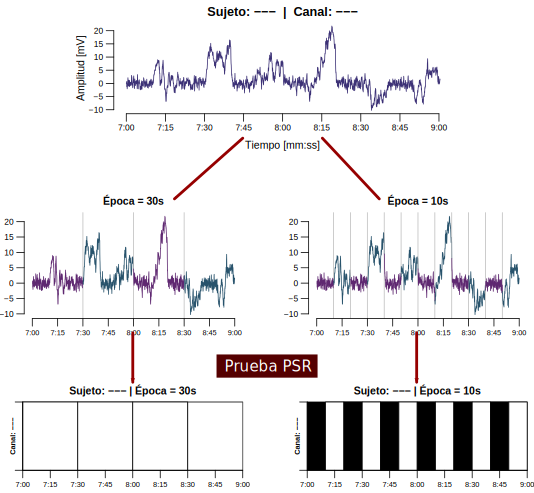
\includegraphics[width=\linewidth]{./img_diagramas/epocas_diferentes_v2.pdf}
\caption{Efecto del tamaño de ventana sobre la clasificación de estacionariedad}
\label{epocas_diferentes}
\end{figure}

\begin{figure}
\centering
\includegraphics[width=\linewidth]
{./img_art_dfa/VCNNS1_comp_est_.png}
\caption{Distribución en el tiempo de ventanas estacionarias, usando diferentes tamaños
de ventana}
\label{comp_VCR}
\end{figure}

Cabe destacar que la aplicación \textit{per se} de la prueba fue efectuada usando el software 
estadístico R \cite{R_citar}. En particular, se utilizó la implementación 
incluida en el paquete \texttt{fractal} \cite{R_fractal} bajo la función \texttt{stationarity}.

%%%%%%%%%%%%%%%%%%%%%%%%%%%%%%%%%%%%%%%%%%%%%%%%%%%%%%%%%%%%%%%%%%%%%%%%%%%%%%%%%%%%%%%%%%%%%%%%%%%
%%%%%%%%%%%%%%%%%%%%%%%%%%%%%%%%%%%%%%%%%%%%%%%%%%%%%%%%%%%%%%%%%%%%%%%%%%%%%%%%%%%%%%%%%%%%%%%%%%%

\section{Espectro de potencias}

Adicionalmente a la clasificación de épocas como estacionarias, se calculó su espectro de potencia. 
Como una metodología común, se calculó el \textbf{espectro de banda ancha},
es decir, la potencia total y relativa correspondientes a las frecuencias que caracterizan las ondas 
delta, theta, alfa, beta y gamma (ver cuadro \ref{tabla_ondas}).

\begin{figure}
\centering
\includegraphics[width=\linewidth]
{./img_art_dfa/VCNNS1_espectral_total.png} 
\caption[Espectro de potencias de banda ancha]{Espectro de potencias de banda ancha (delta, theta
alfa, beta, gamma)}
\end{figure}

Usando los espectros de banda ancha se ha calculado el coeficiente de enlentecimiento \lento, 
definido en la 
expresión \ref{enlentecimiento}, con particular atención al sueño MOR. Esta cantidad
se ha reportado como un posible marcador de deterioro cognitivo leve en adultos mayores 
\cite{Brayet16}.

\begin{equation}
\text{R}_{\text{E}} = \frac{\text{potencia}_{\delta}+\text{potencia}_{\theta}}
{\text{potencia}_{\alpha}+\text{potencia}_{\beta}} =
\frac{\int_{\text 0.5 \hz}^{\text{7 \hz}}h(\omega) d\omega}
{\int_{\text 7 \hz}^{\text{30 \hz}}h(\omega) d\omega}
\label{enlentecimiento}
\end{equation}

El espectro de potencias se ha calculado usado el estimador adaptativo propuesto por
Barbour y Parker \cite{Barbour14}, el cual se encuentra implementado dentro del paquete
\texttt{psd} bajo la función \texttt{pspectrum}.
Se ha usado dicho estimador para garantizar heurísticamente que el espectro de potencias
calculado (1) es independiente del usado para determinar la estacionariedad y (2)
es compatible con la metodología \textit{usual}; como el algoritmo \texttt{psd} 
supone estacionariedad débil se espera que emulae resultados 
obtenidos bajo tal supuesto.

Como se discute posteriormente, los bloques de épocas estacionarias están relacionados a bloques
cuyo espectro de potencia son distintos. Así mismo son diferentes los coeficientes \lento calculado
para dichos bloques.

%%%%%%%%%%%%%%%%%%%%%%%%%%%%%%%%%%%%%%%%%%%%%%%%%%%%%%%%%%%%%%%%%%%%%%%%%%%%%%%%%%%%%%%%%%%%%%%%%%%
%%%%%%%%%%%%%%%%%%%%%%%%%%%%%%%%%%%%%%%%%%%%%%%%%%%%%%%%%%%%%%%%%%%%%%%%%%%%%%%%%%%%%%%%%%%%%%%%%%%
%%%%%%%%%%%%%%%%%%%%%%%%%%%%%%%%%%%%%%%%%%%%%%%%%%%%%%%%%%%%%%%%%%%%%%%%%%%%%%%%%%%%%%%%%%%%%%%%%%%

%%%%%%%%%%%%%%%%%%%%%%%%%%%%%%%%%%%%%%%%%%%%%%%%%%%%%%%%%%%%%%%%%%%%%%%%%%%%%%%%%%%%%%%%%%%%%%%%%%%%
%%%%%%%%%%%%%%%%%%%%%%%%%%%%%%%%%%%%%%%%%%%%%%%%%%%%%%%%%%%%%%%%%%%%%%%%%%%%%%%%%%%%%%%%%%%%%%%%%%%
%%%%%%%%%%%%%%%%%%%%%%%%%%%%%%%%%%%%%%%%%%%%%%%%%%%%%%%%%%%%%%%%%%%%%%%%%%%%%%%%%%%%%%%%%%%%%%%%%%%

\chapter{Resultados}

Previo al análisis de la estacionariedad, se corroboró la hipótesis de que las variables 
independientes son estadísticamente iguales entre los grupos CTL y PDC. Las comparaciones
usando la prueba $t$ de Welch (cuadro \ref{var_ind}) indican que efectivamente la hipótesis se cumple salvo
para los puntajes de Neuropsi.

Se evalúo si pudieran existir relaciones entre las variables que se presumen independientes.
Usando la prueba de correlación de Spearman (cuadro \ref{cor_ind}) se encontró sólo hay 
correlaciones monotónicas entre los siguientes pares de variables:
\begin{itemize}
\item Edad y Escolaridad
\item Puntaje en Neuropsi y Puntaje en Mini Mental-State Examination (MMSE)
\item Tiempo de MOR (en segundos) y Tiempo en MOR (porcentaje)
\end{itemize}

La primera relación, no muy fuerte, puede explicarse como un \textit{efecto generacional}: la educación 
superior ha aumentado su cobertura durante las últimas décadas, y entonces los grupos poblacionales 
más jóvenes tienen en promedio más años de escolaridad. 
%
Algunos autores han sugerido que un bajo nivel de escolaridad es un factor de riesgo para padecer
deterioro cognitivo, en base a estudios horizontales de larga escala \cite{Mejia_Arango2007}.
%
En el presente trabajo se ignora este dato, en vista de que no se pudieron relacionar el nivel de 
escolaridad de los participantes con su desempeño en pruebas neuropsicológicas.

La relación entre los puntajes en Neuropsi y en MMSE era de esperarse, ya que ambas pruebas miden
parámetros similares y tienen contenidos independientes. Cabe mencionar el curioso fenómeno en que (1) 
los puntajes de MMSE
tienen estadísticamente las mismas medias grupales, (2) los puntajes de MMSE están 
fuertemente correlacionados con los puntajes de Neuropsi, y (3) los puntajes de Neuropsi
tienen estadísticamente medias grupales diferentes. Se confirma que la prueba MMSE
tiene menor sensibilidad que la prueba Neuropsi para detectar deterioro cognitivo.

Era por demás obvia la relación entre la cantidad total de sueño MOR, con su proporción respecto a 
todo el sueño. Sin embargo, conviene mencionar que la cantidad de sueño MOR no es afectada por
ninguna de las otras variables independientes; luego entonces las cantidades que fueron estudiadas
(estacionariedad, espectro de potencias) no tienen correlaciones sesgadas con las demás variables.

\begin{table}
\centering
\caption{Variables independientes entre grupos}
\begin{tabular}{lrlcrlcccc}
\toprule
 & \multicolumn{2}{l}{Grupo CTL} & \phantom{.} & \multicolumn{2}{l}{Grupo PDC} 
 & \phantom{.} & \multicolumn{3}{l}{t de Welch}
 \\
\cmidrule{2-3} \cmidrule{5-6} \cmidrule{8-10}
& Media & (DE) & & Media & (DE) & & $p$ & $t$ & $\nu$ \\
\midrule
Edad              &  68.2   & (7.2)     & &    67.6 & (3.4)     & & 0.8746 & 0.16 & 6.11 \\
Escolaridad       &   9.2   & (2.7)     & &     8.4 & (2.2)     & & 0.6201 & 0.52 & 7.69 \\
Neuropsi          & 108.9   & (5.2)     & &    87.8 & (5.6)     & & \bf 0.0003 & 6.17 & 7.94 \\
MMSE              &  29.4   & (0.9)     & &    27.4 & (1.4)     & & 0.0706 & 0.16 & 6.11 \\
Sueño [s]         & 7:51:30 & (0:57:36) & & 7:16:48 & (2:24:43) & & 0.6836 & 0.50 & 5.24 \\
MOR [s]           & 0:52:06 & (0:23:00) & & 0:34:18 & (0:22:14) & & 0.2486 & 1.24 & 7.99 \\
MOR [\%]          &  11.3   & (5.1)     & &     8.4 & (4.8)     & & 0.3871 & 0.91 & 7.96 \\
\bottomrule 
\multicolumn{5}{l}{DE=Desviación Estándar}
\end{tabular} 
\label{var_ind}
\end{table}

\begin{table}
\centering
\caption{Correlaciones entre variables independientes}
\begin{tabular}{llllllll}
\toprule
  &             & 1 & 2 & 3 & 4 & 5 & 6 \\
\midrule
1 & Edad        & $\bullet$  &          &           &          &          & \\
2 & Escolaridad & -0.7134* &  $\bullet$ &           &          &          & \\
3 & Neuropsi    & -0.2432  & \phm 0.3776  & $\bullet$   &          &          & \\
4 & MMSE        & -0.1063  & \phm 0.1812  & 0.8477*** & $\bullet$  &          & \\
5 & Sueño [s]   & \phm  0.0486  & -0.0944  & 0.0545    & 0.0374   & $\bullet$  & \\
6 & MOR [s]     & \phm 0.2796  & -0.5035  & 0.1879    & 0.2618   & -0.1515  & $\bullet$ \\
7 & MOR [\%]    & \phm 0.3709  & -0.5287  & 0.0182    & 0.0748   & -0.3578  & 1**** \\
\bottomrule
\multicolumn{7}{l}{Niveles de significancia: *$<$.05 , **$<$.01 , ***$<$.005 , ****$<$.001}
\end{tabular}
\label{cor_ind}
\end{table}

%%%%%%%%%%%%%%%%%%%%%%%%%%%%%%%%%%%%%%%%%%%%%%%%%%%%%%%%%%%%%%%%%%%%%%%%%%%%%%%%%%%%%%%%%%%%%%%%%%%
%%%%%%%%%%%%%%%%%%%%%%%%%%%%%%%%%%%%%%%%%%%%%%%%%%%%%%%%%%%%%%%%%%%%%%%%%%%%%%%%%%%%%%%%%%%%%%%%%%%

\section{Estacionariedad en sueño MOR}

Se sometió a prueba la hipótesis de que durante sueño MOR ocurre en mayor medida la estacionariedad
débil, en comparación con el sueño NMOR. Para ello, se compararon el porcentaje de épocas 
estacionarias en el sentido de PSR, ocurridas durante sueño MOR y NMOR. La comparación fue efectuada
usando la prueba $\chi^{2}$ de Pearson. Se encontró
de manera consistente que los canales ROG y LOG presentaron diferencias significativas ($p<0.05$) 
entre sueño MOR y NMOR, lo cual puede explicarse por los movimientos oculares rápidos característicos
del sueño MOR. En los canales que corresponden al EEG no se encontraron patrones consistentes y 
claros entre los sujeto (ver figura \ref{cabeza_new}).

\begin{figure}
\centering
\begin{tabular}{ccccc}
VCR & MJH & JAE & GHA & MFGR \\
\includegraphics[width=0.17\textwidth]{./img_art_dfa/cabeza_new_VCR_30.pdf} &
\includegraphics[width=0.17\textwidth]{./img_art_dfa/cabeza_new_MJH_30.pdf} &
\includegraphics[width=0.17\textwidth]{./img_art_dfa/cabeza_new_JAE_30.pdf} &
\includegraphics[width=0.17\textwidth]{./img_art_dfa/cabeza_new_GHA_30.pdf} &
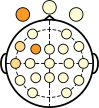
\includegraphics[width=0.17\textwidth]{./img_art_dfa/cabeza_new_MFGR_30.pdf} \\
\midrule
CLO & RLO & RRU & JGZ & AEFP \\
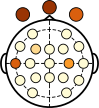
\includegraphics[width=0.17\textwidth]{./img_art_dfa/cabeza_new_CLO_30.pdf} &
\includegraphics[width=0.17\textwidth]{./img_art_dfa/cabeza_new_RLO_30.pdf} &
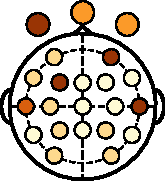
\includegraphics[width=0.17\textwidth]{./img_art_dfa/cabeza_new_RRU_30.pdf} &
\includegraphics[width=0.17\textwidth]{./img_art_dfa/cabeza_new_JGZ_30.pdf} &
\includegraphics[width=0.17\textwidth]{./img_art_dfa/cabeza_new_AEFP_30.pdf} \\
\end{tabular} \\
\includegraphics[scale=.7]{./img_art_dfa/escala.pdf} \\
\caption{Regiones donde la cantidad de ventanas estacionarias es significativamente diferente 
durante sueño MOR y NMOR, usando ventanas de 30 segundos}
\label{cabeza_new}
\end{figure}

Se repitió la comparación a un nivel grupal, usando la prueba $U$ de  Mann-Whitney.
Se encontraron diferencias significativas para el grupo CTL en los canales P3, P4, PZ, 
ROG y EMG; en el grupo PDC se observaron tales diferencias sólo en P4.
%
Las proporciones muestran tendencias que, quizá, resultaron no ser significativas
por el tamaño pequeño de la muestra: los canales P3 y PZ podrían ser diferentes también para
individuos del grupo PDC, y el canal LOG podría ser diferente durante sueño MOR y NMOR.
%
Así mismo se hipotetiza que para el grupo CTL, en todos los canales, el sueño MOR
es presenta menor cantidad de épocas estacionarias.

Se concluye que
no se puede establecer diferencias entre las medias grupales para esta cantidad (proporción de
épocas estacionarias, medidas en el sentido de PSR), debido a la gran variabilidad entre sujetos.

\begin{figure}
\centering
\includegraphics[width=\linewidth]
{./img_art_dfa/Comparacion_gpos_CTL_PDC_v3.pdf}
\caption{Proporciones de épocas estacionarias, durante sueño MOR y NMOR.}
\label{comparacion_verde}
\end{figure}

\begin{figure}
\centering
\includegraphics[width=\linewidth]
{./img_art_dfa/Comparacion_gpos_MOR_NMOR_v3.pdf}
\caption{Proporciones de épocas estacionarias, grupos CTL y PDC.}
\label{comparacion_graf}
\end{figure}

%%%%%%%%%%%%%%%%%%%%%%%%%%%%%%%%%%%%%%%%%%%%%%%%%%%%%%%%%%%%%%%%%%%%%%%%%%%%%%%%%%%%%%%%%%%%%%%%%%%
%%%%%%%%%%%%%%%%%%%%%%%%%%%%%%%%%%%%%%%%%%%%%%%%%%%%%%%%%%%%%%%%%%%%%%%%%%%%%%%%%%%%%%%%%%%%%%%%%%%
%%%%%%%%%%%%%%%%%%%%%%%%%%%%%%%%%%%%%%%%%%%%%%%%%%%%%%%%%%%%%%%%%%%%%%%%%%%%%%%%%%%%%%%%%%%%%%%%%%%

\section{Discusión}

%Una práctica común en el análisis de señales electrofisiológicas es el suponer que una serie de 
%tiempo \textit{suficientemente} corta pueda considerarse estacionaria, cuando menos en el sentido
%débil; anteriormente se ha señalado que se trata de un efecto de muestras pequeñas \cite{Melard89},
%y paralelamente se han incorporado a los diseños experimentales motivos para mantener este supuesto
%\cite{Kaiser00}.
%
%Este trabajo parte de la hipótesis de que adultos mayores con PDC presentan en mayor medida 
%estacionariedad débil en sus registros de PSG; al comparar sujetos de los grupo Nn (control) y Mn 
%(PDC), no se observaron cambios significativos en la porción de tiempo durante la cual el registro 
%de PSG se comporta como débilmente estacionario. 
%Esto puede interpretarse como que los cambios en la corteza cerebral durante el deterioro 
%cognitivo, no provocan que  la señal se vuelva más \textit{simple} en el sentido de 
%\textit{volverse} estacionaria.
%
%Comparando grupalmente la cantidad de épocas estacionarias durante MOR y NMOR, se encontró que en 
%el grupo Nn había diferencias significativas en sitios de la región frontal y que no eran presentes
%en el grupo Mn; para poder establecer una relación con el PDC haría falta un mayor grupo muestral, 
%o bien nuevos registros de PSG para los mismos sujetos, o incluso analizar registros de EEG durante 
%otro tipo de actividades y confirmar las diferencias encontradas.
%
%Cabe destacar que la evidencia aportada indica que el PSG es un conjunto de señales que se comportan
%como no-estacionarias durante la mayor parte del sueño, lo cual confirma el supuesto usual de que 
%las señales de origen biológico son por naturaleza no-estacionarias. 

%\subsection{Efecto del tamaño de las época}

%En el apéndice X se explica que si disminuye el tamaño de época el test de PSR disminuye su 
%potencia, de modo que es más propensa a dar falsos negativos (rechazar la hipótesis de 
%estacionariedad cuando debía aceptarse); entonces, en épocas más pequeñas debería haber más épocas 
%clasificadas como no-estacionarias.
%Sin embargo, al \textit{graficar} la estacionariedad para diferentes tamaños de época (figura
%\ref{comp_VCR}) ocurre que es más frecuente el efecto contrario.
%
%\begin{figure}
%\centering
%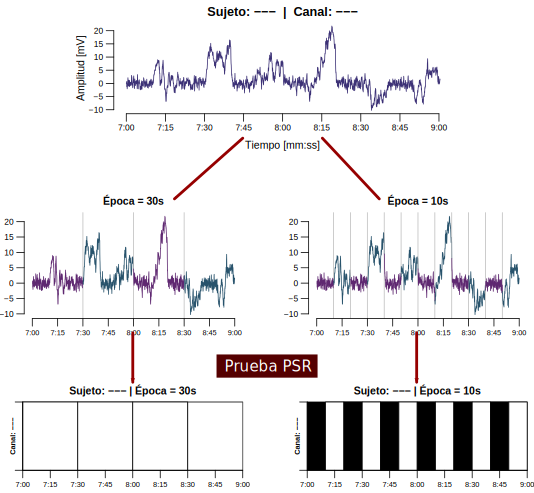
\includegraphics[width=\linewidth]{./img_diagramas/epocas_diferentes_v2.pdf}
%\caption{Efecto del tamaño de ventana sobre la clasificación de estacionariedad}
%\label{epocas_diferentes}
%\end{figure}
%
%Se propone que este efecto puede ser explicado si los registros de PSG son \textbf{localmente
%estacionarios}, una propiedad introducida por Dahlhaus \cite{Dahlhaus97} y que consiste en que un
%proceso no-estacionario pueda ser aproximado a trozos \textit{ensamblando} procesos estacionarios
%definidos para intervalos pequeños de tiempo.
%Esta caracterización del EEG ha sido usada anteriormente de manera fructífera pero problemática
%[??].
%
%En el contexto particular del presente trabajo, la presencia de estacionariedad local puede ser
%explicada fisiológicamente por el contenido heterogéneo de ritmos cerebrales de las etapas de 
%sueño; como ejemplo, en la etapa N3 aparecen husos de sueño mezcladas con ritmos Alfa, de modo
%que es posible hallar un fragmento de época en sueño N3 con únicamente un tren de ondas Alfa
%o un tren de husos de sueño.
%Este fenómeno es ilustrado de manera esquemática en la figura \ref{epocas_diferentes}.
%
%
%
%Entonces, se propone que los registros de PSG se comportan como procesos localmente estacionarios; 
%más aún, se propone que esta característica cambia cualitativamente en adultos mayores con PDC,
%para los cuales el \textit{nivel de homogeneidad} del PSG es muy similar durante MOR y NMOR.

%%%%%%%%%%%%%%%%%%%%%%%%%%%%%%%%%%%%%%%%%%%%%%%%%%%%%%%%%%%%%%%%%%%%%%%%%%%%%%%%%%%%%%%%%%%%%%%%%%%
%%%%%%%%%%%%%%%%%%%%%%%%%%%%%%%%%%%%%%%%%%%%%%%%%%%%%%%%%%%%%%%%%%%%%%%%%%%%%%%%%%%%%%%%%%%%%%%%%%%

\section{Conclusiones}

Se concluye que
es posible la ocurrencia de fragmentos arbitrariamente cortos de registros de PSG que no 
son débilmente estacionarios. Paralelamente, la presencia de estos fragmentos se ve influida por el
estado de actividad del cerebro.
%
Como consecuencia directa de este fenómeno, es posible limitar los efectos \textit{distorsivos} de 
la no-estacionariedad, para lo cual basta un diseño experimental que distinga adecuadamente el
estado de actividad a estudiar. 

En otro ámbito, es en principio posible usar la
proporción de estacionariedad (\textit{densidad} de ventanas estacionarias en el sentido de
PSR) en el EEG para caracterizar estados de actividad cerebral. Para ello, falta 
investigar las características particulares de la etapa que se busca identificar, así como otras
etapas cercanas en el tiempo.

%%%%%%%%%%%%%%%%%%%%%%%%%%%%%%%%%%%%%%%%%%%%%%%%%%%%%%%%%%%%%%%%%%%%%%%%%%%%%%%%%%%%%%%%%%%%%%%%%%%
%%%%%%%%%%%%%%%%%%%%%%%%%%%%%%%%%%%%%%%%%%%%%%%%%%%%%%%%%%%%%%%%%%%%%%%%%%%%%%%%%%%%%%%%%%%%%%%%%%%

\section{Trabajo a futuro}

Una vez que se ha identificado un marcador para el PDC usando un grupo de laboratorio,
conviene automatizar los análisis para su uso clínico sobre un público más general.
%
Un uso más amplio de la técnica asegura una mayor población para poder estudiar la 
efectividad y sensibilidad de la prueba
Y más que eso, se espera que puedan ser sinceramente beneficiosos para los pacientes. Siguiendo el
protocolo usual, los marcadores presentados no serán usados como único recurso para generar
un diagnóstico clínico, sino como un apoyo a las herramientas existentes.

El uso de marcadores basados en registros de PSG --basados en el EEG en general-- aporta una
base fisiológica al diagnóstico de deterioro cognitivo, misma que no es posible usando
únicamente pruebas neuropsicológicas.
%
Conviene destacar que, de entre las herramientas para el registro fisiológico del sistema nervioso
central, las técnicas electrofisiológicas son las más económicas y menos invasivas;
generar marcadores basados en ellas facilita su uso por el público general como herramienta 
diagnóstica, sobre todo en ausencia de síntomas.

%%%%%%%%%%%%%%%%%%%%%%%%%%%%%%%%%%%%%%%%%%%%%%%%%%%%%%%%%%%%%%%%%%%%%%%%%%%%%%%%%%%%%%%%%%%%%%%%%%%
%%%%%%%%%%%%%%%%%%%%%%%%%%%%%%%%%%%%%%%%%%%%%%%%%%%%%%%%%%%%%%%%%%%%%%%%%%%%%%%%%%%%%%%%%%%%%%%%%%%
%%%%%%%%%%%%%%%%%%%%%%%%%%%%%%%%%%%%%%%%%%%%%%%%%%%%%%%%%%%%%%%%%%%%%%%%%%%%%%%%%%%%%%%%%%%%%%%%%%%


\appendix

%%%%%%%%%%%%%%%%%%%%%%%%%%%%%%%%%%%%%%%%%%%%%%%%%%%%%%%%%%%%%%%%%%%%%%%%%%%%%%%%%%%%%%%%%%%%%%%%%%%%
%%%%%%%%%%%%%%%%%%%%%%%%%%%%%%%%%%%%%%%%%%%%%%%%%%%%%%%%%%%%%%%%%%%%%%%%%%%%%%%%%%%%%%%%%%%%%%%%%%%
%%%%%%%%%%%%%%%%%%%%%%%%%%%%%%%%%%%%%%%%%%%%%%%%%%%%%%%%%%%%%%%%%%%%%%%%%%%%%%%%%%%%%%%%%%%%%%%%%%%
%%%%%%%%%%%%%%%%%%%%%%%%%%%%%%%%%%%%%%%%%%%%%%%%%%%%%%%%%%%%%%%%%%%%%%%%%%%%%%%%%%%%%%%%%%%%%%%%%%%

%\chapter{Espectro evolutivo}

\chapter{Variables aleatorias}

Debido al enfoque de aplicación para el presente trabajo, ha sido necesario incluir explicaciones
pragmáticas y cortas. 
Sin embargo, conviene enfatizar que los objetos
matemáticos son más que herramientas para analizar datos: son definidos formalmente dentro
de un sistema axiomático y tienen propiedades objetivas.

En este anexo se exhiben algunas definiciones y teoremas implicados, pero que no tienen una 
repercusión directa sobre la parte procedimental de la metodología.
%
Paralelamente, introducir la terminología adecuada permitirá entender los análisis realizados y 
los resultados obtenidos.

%%%%%%%%%%%%%%%%%%%%%%%%%%%%%%%%%%%%%%%%%%%%%%%%%%%%%%%%%%%%%%%%%%%%%%%%%%%%%%%%%%%%%%%%%%%%%%%%%%%
%%%%%%%%%%%%%%%%%%%%%%%%%%%%%%%%%%%%%%%%%%%%%%%%%%%%%%%%%%%%%%%%%%%%%%%%%%%%%%%%%%%%%%%%%%%%%%%%%%%

\section{Medidas}

%Un primer motivo para esta sección es enfatizar que, formalmente, una variable aleatoria se concibe 
%como un espacio de medida y no como un recuento de eventos. 

\begin{definicion}[$\boldsymbol{\sigma}$-álgebra]
Sea $U$ un conjunto y $\mathcal{U}$ una colección de subconjuntos de $U$. Se dice que $\mathcal{U}$
es una $\sigma$-álgebra si cumple que
\begin{itemize}
\item $U \in \mathcal{U}$
\item $A \in \mathcal{U}$ implica que $A^{C} \in \mathcal{U}$
\item Si $\{ A_n \}_{n\in \mathbb{N}}$ son conjuntos tales que $A_i \in \mathcal{U}$, entonces
$\displaystyle \cup_{n\in \mathbb{N}} A_n \in \mathcal{U}$
\end{itemize}
Donde $A^{C}$ es el complemento $\{ u \in U | u \notin A \} $
\end{definicion}

Por simplicidad, en este trabajo sólo se usarán medidas para conjuntos de números reales derivadas 
de la $\sigma$-álgebra de Borel, que es definida como la $\sigma$-álgebra más pequeña que contiene a 
los intervalos abiertos abiertos\footnote{Si una $\sigma$-álgebra contiene a todos los
intervalos abiertos, entonces debe contener a todos los elementos de la $\sigma$-álgebra de Borel}.

\begin{definicion}[Medida]
Sea $U$ un conjunto y $\mathcal{U}$ una $\sigma$-álgebra definida en $U$. Se dice que una función
$\mu : \mathcal{U} \rightarrow \R \cup {\infty}$ es una medida si cumple que
\begin{itemize}
\item $\mu(\emptyset) = 0$
\item $\mu(A) \geq 0$ para cualquier $A \in \mathcal{U}$
\item Si $\{ A_n \}_{n\in \mathbb{N}}$ son conjuntos disjuntos a pares y tales que 
$A_i \in \mathcal{U}$, entonces 
$\displaystyle \mu\left( \cup_{n\in \mathbb{N}} A_n \right) = \sum_{n\in \mathbb{N}} \mu(A_n)$
\end{itemize}
Donde $\emptyset$ es el conjunto vacío %y $\R^{*} = \R \cup \{-\infty,\infty \}$
\end{definicion}

\begin{definicion}[Medida de probabilidad en $\boldsymbol{\R}$]
Sea $\mathcal{B}$ la sigma álgebra de Borel definida para $\R$, se dice que una función
$P : \mathcal{B} \rightarrow [0.1]$ es una \textbf{medida de probabilidad} si cumple que
\begin{itemize}
\item $P(\emptyset) = 0$
\item $0 \leq P(A) \leq 1$ para cualquier $A \in \mathcal{B}$
\item Si $A, B \in \mathcal{B}$ y $A\cap B = \emptyset$, entonces $P(A \cup B) = P(A) + P(B)$ 
\item $P(\R) = 1$
\end{itemize}
\label{variable_aleatoria}
\end{definicion}

%Cabe mencionar que cuando se usa una variable aleatoria para modelar un fenómeno, existe un paso
%intermedio en que los eventos relevantes se asocian con números reales

Otra forma de entender una variables aleatoria es a partir de su función de probabilidad
acumulada (FPA), ya que hay una correspondencia unívoca entre cada variable aleatoria y su FPA.

\begin{definicion}[Función de Probabilidad Acumulada]
Sea 
\begin{equation*}
F_X (x) = P\left( (-\infty,x] \right)
\end{equation*}
\end{definicion}

Habitualmente, como se hace el presente texto, se usa el símbolo $X$ para denotar a una variable 
aleatoria cuya FPA es $F_X$. Bajo esta idea, para cualquier conjunto $I \subseteq \R$ se denota
$P(X \in I) = P(I)$, una notación muy extendida.



\begin{teorema}[Descomposición de Lebesgue]
Sea $f:I\rightarrow \R$ una función de variación acotada, con $I$ un intervalo. Entonces pueden 
hallarse funciones $f_j, f_c, f_a :I\rightarrow \R$ tales que
\begin{itemize}
\item $f = f_j+ f_c+ f_a$
\item $f_j = \sum_{y \leq x} f(x-0) + f(x+0)$
\item $f_a$ es absolutamente continua\footnote{Para que una función sea absolutamente continua,
basta que sea de variación acotada y que mapee conjuntos de medida cero en conjuntos de medida
cero} en $I$
\item $f_c$ es una función singular\footnote{Una función es singular si es continua, de 
variación acotada y no-constante, y se cumple que tiene derivada cero casi en todas partes} en 
$I$
\end{itemize}
Estas funciones son únicas excepto por constantes, y en conjunto son llamados la 
\textit{descomposición de Lebesgue} de $f$
\label{Lebesgue_decomp}
\end{teorema}

%%%%%%%%%%%%%%%%%%%%%%%%%%%%%%%%%%%%%%%%%%%%%%%%%%%%%%%%%%%%%%%%%%%%%%%%%%%%%%%%%%%%%%%%%%%%%%%%%%%

\section{Procesos estocásticos}

%\begin{definicion}[Proceso estocástico]
%Un proceso estocástico \xt es una familia de variables aleatorias reales, 
%indexadas por $t \in T$.
%\label{proc_estocastico}
%\end{definicion}
%
%Respecto al conjunto $T$ que indexa a un proceso estocástico, y que será referido como 
%\textit{tiempo}, conviene introducir dos grandes grupos para los mismos
%\begin{itemize}
%\item \textit{Continuo} si $T$ es un intervalo cerrado
%\item \textit{Discreto} si $T$ es de la forma 
%$\{ t_0 + n \delta \lvert n \in U \subseteq \mathbb{Z} \}$
%\end{itemize}
%
%Los procesos a tiempo discreto contemplan conjuntos finitos e infinitos de puntos en el tiempo.
%No se manejan discutirá sobre otros tipos de tiempo en este trabajo.
%
%Como notación, se usará \xt  para el proceso estocástico y $X(t)$ para una de las variables
%aleatorias que lo componen; de la misma manera $x(t)$ es una realización de $X(t)$ y $F_{X(t)}$ 
%es la función de probabilidad acumulada para $X(t)$.



\begin{definicion}[Continuidad estocástica en media cuadrática]
Un proceso estocástico a tiempo continuo $\{ X(t) \}$ es estocásticamente continuo, en el 
sentido de media cuadrática, en un tiempo admisible $t_0$ si y sólo si
\begin{equation*}
\lim_{t \rightarrow t_0} \E{\left( X(t) - X(t_0) \right)^{2}} = 0
\end{equation*}
\label{cont_est}
\end{definicion}

Una forma natural de pensar en la definición \ref{cont_est} es que, si $\abso{t-t_0}$ es muy 
pequeño, entonces $X(t)$ y $X(t_0)$ difieren muy poco entre s\'i (como variables aleatorias).
Es destacable que si un proceso es estocásticamente continuo en un intervalo, sus realizaciones 
solamente se pueden garantizar continuas casi en todas partes \footnote{Una propiedad se cumple 
\textbf{casi en todas partes} si se cumple en un conjunto cuyo complemento tiene medida cero} en 
ese intervalo.

Como ejemplos, un proceso ruido blanco (definición \ref{r_blanco}) no es estocásticamente 
continuo, mientras que un proceso de Wiener (definición \ref{r_wiener}) s\'i lo es.

\begin{definicion}[Proceso ruido blanco]
Se dice de un proceso estocástico $\{ R(t) \}$ que cumple, para cualesquiera tiempos admisibles
$t$ y $s$, las siguientes propiedades:
\begin{itemize}
\item $\E{R(t)}=0$
\item $\Cov{R(t),R(s)}=0 \Leftrightarrow t=s$ 
\end{itemize}
\label{r_blanco}
\end{definicion}

\begin{definicion}[Proceso de Wiener]
Se dice de un proceso estocástico $\{ W(t) \}$ que cumple, para cualesquiera tiempos admisibles
$t$ y $s$ (con $s>t$) las siguientes propiedades:
\begin{itemize}
\item $W(0) = 0$ ($W(0)$ es constante)
\item $W(s)-W(t)$ es independiente de $W(u)$, para todo $u<t$ admisible
\item $W(s)-W(t) \sim N(0,\abso{t-s})$  (los incrementos tienen distribución normal)
\end{itemize}
\label{r_wiener}
\end{definicion}

\begin{definicion}[Estacionariedad débil]
Un proceso estocástico \xt es débilmente estacionario si y sólo si para cualesquiera tiempos 
admisibles\footnote{El término \textit{tiempos admisibles} significa que la definición es la misma
para diferentes tipos de tiempo, bajo las restricciones pertinente} $t$, $s$ se tiene que
\begin{itemize}
\item $\E{X(t)} = \mu_X$
\item $\Var{X(t)} = \sigma^{2}_X$
\item $\Cov{X(t),X(s)} = \rho_X (s-t)$
\end{itemize}
Donde $\mu_X$, $\sigma^{2}_X$ son constantes, $\rho_X(\tau)$ es una función que únicamente 
depende de $\tau$
\label{est_orden_primera}
\end{definicion}

\section{Transformada de Fourier como operador}

La exposición inicia con los espacios de las \textbf{series $\boldsymbol{p}$-sumables}
($\lp$), y las  \textbf{funciones $\boldsymbol{p}$-integrables} sobre un intervalo 
$I \subseteq \R$ ($\llp$).
%; en el presente trabajo sólo se usarán los casos $p=1,2$.
%
%\begin{align}
%\ell^{p} &:= \left\{ s: \Z\rightarrow\C \talque \sum_{n=-\infty}^{\infty} \abso{s(n)}^{p} < \infty \right\}
%\label{lpdef} \\
%L^{p}[I] &:= \left\{ S: I\rightarrow\C \talque \int_I \abso{S(t)}^{p} dt < \infty \right\}
%\label{llpdef}
%\end{align}
\begin{align*}
\ell^{p} &:= \left\{ s: \Z\rightarrow\C \talque \sum_{n=-\infty}^{\infty} \abso{s(n)}^{p} < \infty \right\}
\\
L^{p}[I] &:= \left\{ S: I\rightarrow\C \talque \int_I \abso{S(t)}^{p} dt < \infty \right\}
\end{align*}

Estos espacios admiten las operaciones $+$, $\cdot$ y multiplicación por escalares complejos de la 
manera usual.%, es decir

%\begin{align*}
%s, z \in \lp, c \in \C \Rightarrow 
%[s+z](n) &= s(n) + z(n) \\
%[s\cdot z](n) &= s(n) z(n) \\
%[c \cdot s](n) &= s(n)c \\
%S, Z \in \llp, c \in \C \Rightarrow 
%[S+Z](t) &= S(t) + Z(t) \\
%[S\cdot Z](t) &= S(t)  Z(t) \\
%[c \cdot S](t) &= S(t)c
%\end{align*}
%
%En las próximas líneas se seguirán usando $s, z, S, Z, c$.

Para el caso particular $p=2$, los conjuntos $\ldos$ y $\lldos$ admiten los siguientes productos 
internos:
%
\begin{align*}
\left\langle s,z \right\rangle &= \sum_{n=-\infty}^{\infty} s(n) \overline{z(n)}\\
\left\langle S,Z \right\rangle &= \int_I S(t) \overline{Z(t)} dt
\end{align*}

Usando dichos productos internos, junto con las normas y métricas que inducen, los conjuntos 
$\ldos$ y $\lldos$ tienen estructura de \textbf{espacio de Hilbert}.

Con las definiciones anteriores, que muestran que $\ldos$ y $\lldos$ son \textit{muy}
parecidos, se puede formular unas definición para la transformada de Fourier como una equivalencia
entre estos espacios.

%{De manera pragm\'atica, en el presente trabajo la 
%palabra  'frecuencia' se usar\'a para referirse a la cantidad $q$ en expresiones del tipo 
%$e^{i q t}$}

\begin{definicion}[Serie de Fourier]
Sea $S: \R \rightarrow \C$ una función periódica con periodo $2T$ y tal que 
$S \in L^{2}\left[[-T,T]\right]$. Se dice que $A$ es la serie de Fourier para $S$ si cumple que
\begin{equation*}
A(n) = \frac{1}{2 T} \simint{T} S(t) e^{-\nicefrac{ i \abso{n} t}{2T}} dt
\end{equation*}
%Adicionalmente, la función $\mathcal{F} : \lldos \rightarrow \ldos : S \mapsto A$  recibe el nombre
%de \textbf{Transformada de Fourier}
\label{FourierClasico}
\end{definicion}

\begin{definicion}[Transformada de Fourier]
Sean $S$ y $A$ como en la definición \ref{FourierClasico}. Se le llama transformada de Fourier a la
función $\mathcal{F}_T : L^{2}\left[[-T,T]\right] \rightarrow \ldos : S \mapsto A$
\end{definicion}

Puede interpretarse a $A$ como las \textit{coordenadas} de $S$ en $L^{2}\left[[-T,T]\right]$, 
usando una base de funciones $\left\{ e^{\nicefrac{i \abso{n} t}{2 T}} \right\}_{n\in \Z}$, las
cuales resultan ser ortonormales; esta base en particular es conocida como la \textbf{base de 
Fourier}.
Se demuestra en el anexo A que $\mathcal{F_T}$ está bien definida en el sentido de 
tener efectivamente el dominio y codominio indicados. Así mismo, cabe mencionar las siguientes 
propiedades de $\mathcal{F}_T$
\begin{itemize}
\item Es lineal, es decir, $\mathcal{F}_T[cS + Z] = c\mathcal{F}_T[S] + \mathcal{F}_T[Z]$

\item \textbf{No} es invertible, aunque se le suele definir una
pseudoinversa\footnote{$\mathcal{F}_T^{\text{inv}}$ es \textit{exacta} salvo por la suma
de alguna función $S_0$ tal que $\int_{-T}^{T}\abso{S_0(t)}dt = 0$} como
\begin{equation*}
\mathcal{F}_{T}^{\text{inv}} : \ldos \rightarrow L^{2}\left[[-T,T]\right] :
A \mapsto \sum_{n -\infty}^{\infty} A(n) e^{\nicefrac{i \abso{n} t}{2 T}}
\end{equation*}
\end{itemize}

Con esta terminología se define, de manera pragmática, la \textbf{energía disipada} y la 
\textbf{potencia} de una función $S$ en un intervalo $[a,b]$ como 
\begin{align*}
\text{energía}[S]_{[a,b]} &= \int_a^{b} \abso{S(t)}^{2} dt \\
\text{potencia}[S]_{[a,b]} &= \frac{1}{b-a} \int_a^{b} \abso{S(t)}^{2} dt
\end{align*}
%
%Estas últimas definiciones cobran importancia a la luz del teorema \ref{parseval}: la energía de 
%una función equivale a su norma.

Una consecuencia interesante de este concepto de energía frente al teorema \ref{parseval} es que la 
energía disipada por una función equivale a la suma de la energía disipada por sus 
\textit{componentes} en la base de Fourier.
Conviene, entonces, definir una función que \textit{desglose} estos \textit{aportes}.

\begin{teorema}[Parseval]
Sea $S \in L^{2}\left[[-T,T]\right]$, y sea $A = \mathcal{F}[S]$. Se cumple que
\begin{equation*}
\int_{-T}^{T} \abso{S(t)}^{2} dt = \sum_{n=-\infty}^{\infty} \abso{A(n)}^{2}
\end{equation*}
\label{parseval}
\end{teorema}

\begin{definicion}[Espectro de potencias]
Sea $S \in L^{2}\left[[-T,T]\right]$, y sea $A = \mathcal{F}[S]$. Se llama espectro de potencias 
para $S$ a la función $h_S : \R \rightarrow \R $, definida como
\begin{equation*}
h_S(\omega) = 
\begin{cases}
\abso{A(n)}^{2} & \text{ , si } \omega = \nicefrac{n}{2T}, \text{   con } n\in \mathbb{Z} \\
0 & \text{ ,  otro caso}
\end{cases}
\end{equation*}
\label{espec}
\end{definicion}

Un elemento que será de crucial importancia en el desarrollo posterior es la \textbf{convolución}, 
$\ast$, una tercera operación binaria definida en estos espacios como
%
\begin{align*}
[s \ast z] (\tau) &= \sum_{n=-\infty}^{\infty} s(n) \overline{z(\tau-n)} \\
[S \ast Z] (\tau) &= \int_I S(t) \overline{Z(\tau-t)}
\end{align*}
%
donde $\overline{c}$ es el conjugado complejo de $c$. 
%La convolución es conmutativa y asociativa con la suma. 
Esta operación cobra importancia por la forma en que se relaciona con $\mathcal{F}_T$
%
\begin{teorema}%[de la convolución]
Sean $S,Z \in L^{2}\left[[-T,T]\right]$, entonces se satisface que
\begin{align*}
\mathcal{F}_T[S\ast Z]  &= \mathcal{F}_T[S] \cdot \mathcal{F}_T[Z] \\
\mathcal{F}_T[S\cdot Z] &= \mathcal{F}_T[S] \ast  \mathcal{F}_T[Z] \\
\end{align*}
\label{t_convolucion}
\end{teorema}

%%%%%%%%%%%%%%%%%%%%%%%%%%%%%%%%%%%%%%%%%%%%%%%%%%%%%%%%%%%%%%%%%%%%%%%%%%%%%%%%%%%%%%%%%%%%%%%%%%%

\section{Representación espectral}

\begin{teorema}
Sea $\{X(t)\}$ un proceso estocástico a tiempo continuo débilmente estacionario de media 0 y 
estocásticamente continuo en el sentido de media cuadrática. Entonces, existe un proceso 
ortogonal $\{Z(\omega)\}$ tal que, para todo tiempo $\omega$ admisible, se puede 
escribir\footnote{La integral se encuentra definida en el sentido de media cuadrática.}
\begin{equation*}
X(t) = \intR e^{i t \omega} dZ(\omega)
\end{equation*}
Donde el proceso $\{Z(t)\}$ tiene las siguientes propiedades para todo $\omega$
\begin{itemize}
\item $\E{dZ(\omega)} = 0$
\item $\E{\abso{dZ(\omega)}^{2}} = dH(\omega)$
\item $\Cov{dZ(\omega),dZ(\lambda)} = 0 \Leftrightarrow \omega \neq \lambda$
\end{itemize}
Donde $dH(\omega)$ la FDE integrada de $\{X(t)\}$
%\label{rep_espectral}
\end{teorema}

\begin{teorema}[Wiener-Khinchin]
Una condición suficiente y necesaria para que $\rho$ sea una función de autocorrelación de 
algún proceso estocástico a tiempo continuo $\{X(t)\}$ débilmente estacionario y 
estocásticamente continuo, es que exista una función $F$ que tenga las siguientes propiedades
\begin{itemize}
\item Monótonamente creciente
\item $F(-\infty) = 0$
\item $F(+\infty) = 1$
\end{itemize}
y tal que para todo $\tau \in \R$ se cumple que
\begin{equation*}
\rho(\tau) = \intR e^{i \omega \tau} dF(\omega)
\end{equation*}
\label{t_wienerkhinchin}
\end{teorema}

\begin{teorema}[Wold]
Una condición suficiente y necesaria para que $\rho$ sea una función de autocorrelación de 
algún proceso estocástico a tiempo discreto $\{X(t)\}$ débilmente estacionario es que exista 
una función $F$ con las siguientes propiedades
\begin{itemize}
\item Monótonamente creciente
\item $F(-\pi) = 0$
\item $F(+\pi) = 1$
\end{itemize}
y tal que para todo $\tau \in \R$ se cumple que
\begin{equation*}
\rho(\tau) = \intPI e^{i \omega \tau} dF(\omega)
\end{equation*}
\label{t_wold}
\end{teorema}

En virtud del teorema de Wold, se puede tener una variante del teorema de Wiener-Khinchin
para procesos a tiempo discreto, razón por la cual  
tal representación es referida como \textbf{representación de Wold-Cramér}.

En el marco de la estimación del espectro de potencias, 

\begin{proposicion}
Sean $u$ y $v$ dos funciones con las siguientes características
\begin{itemize}
\item $\argmax_x u(x), \argmax_x u(x) \ni 0$
\item $\intR \abso{u(x)} dx, \intR \abso{v(x)} dx < \infty$
\item $\intR x\abso{u(x)} dx, \intR x\abso{v(x)} dx < \infty$
\end{itemize} 
Si además se satisface que $u$ tiene una {concentración} muy alta con relación a $v$
($ \intR \abso{u(x)} dx << \intR \abso{v(x)} dx $),
entonces se cunple que
\begin{equation*}
\intR u(x) v(x+k) dx \approx v(k) \intR u(x) dx
\end{equation*}
\label{pseudo_d}
\end{proposicion}

%Las funciones con las características del teorema \ref{pseudo_d} serán referidas como funciones tipo 
%\textit{pseudo $\delta$ de Dirac}.

%%%%%%%%%%%%%%%%%%%%%%%%%%%%%%%%%%%%%%%%%%%%%%%%%%%%%%%%%%%%%%%%%%%%%%%%%%%%%%%%%%%%%%%%%%%%%%%%%%%

\section{Estimación del espectro evolutivo}

Una vez definido el espectro evolutivo para procesos no-estacionarios con varianza finita, cabe 
preguntarse sobre le estimación de esta cantidad a partir de una realización del proceso usando, 
por ejemplo, periodogramas modificados; tal pregunta no tiene, en general, una respuesta 
satisfactoria.
Es por ello que se define una colección, más restringida, de procesos no-estacionarios cuyo 
espectro evolutivo pueda ser estimado efectivamente usando la técnica de ventanas.

Considerando un proceso no-estacionario \xt que admite una representación de la forma 
$X(t) = \intR A(t,\omega) e^{i \omega t} dZ(\omega)$, entonces el espectro evolutivo queda definido 
como
\begin{equation}
dF_t(\omega) = \abso{A(t,\omega)}^{2} d\mu(\omega)
\label{esp_evolutivo}
\end{equation}

Antes de poder usar la proposición \ref{pseudo_d} para estimar $F_t$ (con respecto a $t$) usando 
una ventana espectral, hay que medir la dispersión de $F_t$ en el tiempo; más aún, hay que pedir 
que esa dispersión sea finita.
Con vista a la ecuación \ref{esp_evolutivo}, se puede usar la conexión entre $F$ y $A$ para 
establecer condiciones respecto a la segunda; se define entonces a $H_\omega$, la transformada de
Fourier de $A$ en el tiempo
\begin{equation}
A(t,\omega) = \intR e^{i t \theta} dH_\omega(\theta)
\end{equation}

Un motivo muy fuerte para definir un objeto tan rebuscado es que (...)

Posteriormente se define a $B_{\mathbf{F}}$, el ancho de banda para $H_\omega$ con respecto a la 
familia de funciones $\mathbf{F}$, como
%
\begin{equation}
B_{\mathbf{F}}(\omega) = \intR \abso{\theta} \abso{dH_\omega(\theta)}
\end{equation}

Se dice que el proceso es semi-estacionario con respecto a $\mathbf{F}$ si 
$\sup_\omega B_{\mathbf{F}} < \infty$. El proceso se dice simplemente \textbf{semi-estacionario} 
si esta cantidad es acotada para cualquier familia de funciones admisibles 
$\mathbf{F} \in \mathbf{C}$; entonces se puede definir la constante $B_X$, el \textit{ancho de 
banda característico de} \xt, como

\begin{equation}
B_X = \sup_{\mathbf{F}\in \mathbf{C}} \left[ \sup_\omega B_{\mathbf{F}}(\omega) \right]^{-1}
\end{equation}

Muy vagamente, $B_X$ indica el tiempo máximo en el cual el proceso, representado en la forma
\ref{esp_evolutivo}, (...)

Una vez definida la cantidad $B_X$, y habiendo supuesto que no es 0, es demostrado en 
\cite{Priestley65} que el estimador $U$ definido como en ... satisface que
%
\begin{equation}
\E{\abso{U(t,\omega)}^{2}} = \intR \abso{\Gamma(\omega)}^{2} f(t,\omega+\omega_0) d\omega
+ \orden\left( \nicefrac{B_g}{B_X} \right)
\end{equation}

De esta última expresión es evidente que el estimador es mejor conforme 
\begin{itemize}
\item  $B_X$, el tiempo máximo para el cual el proceso es \textit{básicamente estacionario}, es 
mayor
\item $B_g$, la dispersión en el tiempo para la ventana $g$, es menor
\end{itemize}

%---
%
%Entonces se ha probado en \cite{Priestley66,Priestley69} que bajo ciertas
%condiciones p

\section{Estimador de doble ventana}

Respecto a la estimación del espectro local se usa el \textbf{estimador de doble ventana}, 
técnica introducida por Priestley \cite{Priestley69} y que requiere dos funciones, $w_\tau$ y 
$g$, que funcionan como ventana de retrasos y como filtro lineal, respectivamente.
%
En cuando a $g$, se define a $\Gamma(u) = \intR g(u) e^{i u \omega} du$ y se les pide que
\begin{equation*}
2\pi \int_{-\infty}^{\infty} \lvert g(u) \lvert^{2} du 
= 
\int_{-\infty}^{\infty} \lvert \Gamma(\omega) \lvert^{2} d\omega
= 1
\end{equation*}

%Cabe mencionar que las ventanas espectrales mostradas en la tabla \ref{ventanas} bien 
%pueden cumplir las propiedades requeridas para ser filtros.
Posteriormente se define el estimador $U$ con el objetivo de asignar pesos en el tiempo para estimar
a la FDE
% en el tiempo dado; más aún, $U$ sirve 
%como una aproximación de la representación de Wold-Cramér para 
%el proceso.
\begin{equation*}
U(t,\omega) = \int_{t-T}^{t} g(u) X({t-u}) e^{i \omega (t-u)} du
\end{equation*}

Bajo el entendido que la función $\Gamma$ converge a una función tipo \dirac, puede 
considerarse que 
$\E{\abso{U(t,\omega)}^{2}} \approx f_t(\omega)$; sin embargo, se demuestra en \cite{Priestley66} 
que $\Var{\abso{U(t,\omega)}^{2}} \nrightarrow 0$.
%
Debido a ello se usa una segunda función tipo ventana,
%, para 'suavizar' el estimador y hacerlo consistente (
de forma similar al periodograma.
Se considera la función $W_\tau$, ventana de retrasos, y su respectiva ventana espectral 
$w_\tau$; deben satisfacer las siguientes propiedades:
\begin{itemize}
\item $w_{\tau}(t) \geq 0$ para cualesquiera $t$, $\tau$
\item $w_{\tau}(t) \rightarrow 0$ cuando $\lvert t \lvert \rightarrow \infty$, para todo $\tau$
\item $\displaystyle \int_{-\infty}^{\infty} w_{\tau}(t) dt = 1$ para todo $\tau$
\item $\displaystyle \int_{-\infty}^{\infty} \left( w_{\tau}(t) \right)^{2} dt < \infty$ para todo $\tau$
\item $\exists C$ tal que  
$\displaystyle \lim_{\tau\rightarrow\infty} \tau \int_{-\infty}^{t} \abso{ W_{\tau}(\lambda) }^{2} d\lambda = C$
\end{itemize}

%Por ejemplo, la ventana de Daniell satisface estas propiedades; para ello, conviene calcular que
%$\lim_{\tau\rightarrow\infty} \tau \int_{t-T}^{t} \lvert W_{\tau}(\lambda) \lvert^{2} d\lambda = 2\pi$;
%más aún, 
%Cabe mencionar que todas las ventanas mostradas en \ref{ventanas} satisfacen las propiedades 
%anteriores.
Finalmente, se define el estimador $\est{f}$ para las FDE normalizada, $f_t$, como
\begin{equation*}
\widehat{f}(t,\omega) = \int_{t-T}^{t} w_{T'}(u) \lvert U(t-u,\omega) \lvert^{2} du
\label{estimador_doble_ventana}
\end{equation*}

Fue demostrado por Priestley \cite{Priestley65} que los estimadores de doble ventana son 
asintóticamente insesgados y consistentes, y propone las siguientes aproximaciones:
%conviene exhibir las siguientes expresiones aproximadas propuestas en aquél trabajo
\begin{itemize}
\item $\displaystyle
\E{\est{f}(t,\omega)} \approx 
\intR \widetilde{f}(t,\omega+\theta) \abso{\Gamma(\theta)}^{2} d\theta$
\item $\displaystyle
\Var{\est{f}(t,\omega)} \approx \frac{C}{\tau} \left( \overline{f}^{2}(\omega) \right)
\intR \abso{\Gamma(\theta)}^{4} d\theta $
\end{itemize}

donde las funciones $\widetilde{f}$ y $\overline{f}$ son versiones 'suavizadas' de la FDE 
normalizada, $f$, y están definidas de la siguiente manera
\begin{equation*}
\widetilde{f}(t,\omega+\theta) = 
\intR W_{\tau}(u) f(t-u,\omega+\theta) du
\end{equation*}
\begin{equation*}
\overline{f}^{2} (t,\omega) =
\frac{\intR f^{2}\left(t-u,W_{\tau}^{2}(u)\right) du}
{\intR \left( W_{\tau}(u) \right)^{2} du}
\end{equation*}

Como $W_{\tau}$ funciona como ventana espectral, converge a una 
función tipo \dirac; luego $\widetilde{f}$ es aproximadamente la convolución 
$\widetilde{f}(t,\omega+\theta) \approx \delta_t \ast f(\bullet,\omega+\theta)$. 
Una aproximación muy similar 
puede hacerse respecto al segundo término, de modo que $\widetilde{f}\approx f$ y 
$\overline{f}^{2}\approx f^{2}$.
Tales aproximaciones serán mejores en tanto las ventanas $w_{\tau}$ y $W_{\tau}$ sean más 
cercanas a funciones tipo \dirac.
%; más aún, una condición adecuada es que estas funciones 
%tengan una forma 'más delgada' que el espacio entre los tiempos y frecuencias donde se estimará 
%$f$.
Dicho esto, se pueden hacer las siguientes aproximaciones, un poco más arriesgadas:
\begin{itemize}
\item $\displaystyle \E{\est{f}(t,\omega)} \approx f(t,\omega)$
\item $\displaystyle \Var{\est{f}(t,\omega)} \approx 
\frac{C}{\tau} f^{2}(t,\omega) \intR \abso{\Gamma (\theta)}^{4} d\theta$
\end{itemize}

%%%%%%%%%%%%%%%%%%%%%%%%%%%%%%%%%%%%%%%%%%%%%%%%%%%%%%%%%%%%%%%%%%%%%%%%%%%%%%%%%%%%%%%%%%%%%%%%%%%
%%%%%%%%%%%%%%%%%%%%%%%%%%%%%%%%%%%%%%%%%%%%%%%%%%%%%%%%%%%%%%%%%%%%%%%%%%%%%%%%%%%%%%%%%%%%%%%%%%%

%\section{Efecto del filtro STL}

%%%%%%%%%%%%%%%%%%%%%%%%%%%%%%%%%%%%%%%%%%%%%%%%%%%%%%%%%%%%%%%%%%%%%%%%%%%%%%%%%%%%%%%%%%%%%%%%%%%
%%%%%%%%%%%%%%%%%%%%%%%%%%%%%%%%%%%%%%%%%%%%%%%%%%%%%%%%%%%%%%%%%%%%%%%%%%%%%%%%%%%%%%%%%%%%%%%%%%%
%%%%%%%%%%%%%%%%%%%%%%%%%%%%%%%%%%%%%%%%%%%%%%%%%%%%%%%%%%%%%%%%%%%%%%%%%%%%%%%%%%%%%%%%%%%%%%%%%%%
%%%%%%%%%%%%%%%%%%%%%%%%%%%%%%%%%%%%%%%%%%%%%%%%%%%%%%%%%%%%%%%%%%%%%%%%%%%%%%%%%%%%%%%%%%%%%%%%%%%

%%%%%%%%%%%%%%%%%%%%%%%%%%%%%%%%%%%%%%%%%%%%%%%%%%%%%%%%%%%%%%%%%%%%%%%%%%%%%%%%%%%%%%%%%%%%%%%%%%%%
%%%%%%%%%%%%%%%%%%%%%%%%%%%%%%%%%%%%%%%%%%%%%%%%%%%%%%%%%%%%%%%%%%%%%%%%%%%%%%%%%%%%%%%%%%%%%%%%%%%
%%%%%%%%%%%%%%%%%%%%%%%%%%%%%%%%%%%%%%%%%%%%%%%%%%%%%%%%%%%%%%%%%%%%%%%%%%%%%%%%%%%%%%%%%%%%%%%%%%%

\chapter{Compilados gráficos}

En este apéndice se muestran los compilados gráficos mencionados en la parte de resultados,
y que representan la
distribución temporal y pseudo-espacial de las ocurrencia de épocas PSG dentro de los registros 
para cada paciente. 

Primeramente se presentan los compilados gráficos en los que se ha destacado el sueño MOR;
posteriormente se presentan los mismos gráficos resaltando los patrones visuales
propuestos, que parecen estar relacionados con la aparición de sueño MOR.

\begin{figure}
\centering
{\small
\begin{tabular}{lccccc}
\toprule
{\small Tamaño de} & \multicolumn{5}{c}{Grupo CTL} \\
    \cmidrule{2-6}
{\small ventana [s]}    & VCR & MJH & JAE & GHA & MFGR \\
\midrule
$30 \times 2^1$ &
\includegraphics[width=0.13\textwidth]{./img_art_dfa/cabeza_new_VCR_60.pdf} &
\includegraphics[width=0.13\textwidth]{./img_art_dfa/cabeza_new_MJH_60.pdf} &
\includegraphics[width=0.13\textwidth]{./img_art_dfa/cabeza_new_JAE_60.pdf} &
\includegraphics[width=0.13\textwidth]{./img_art_dfa/cabeza_new_GHA_60.pdf} &
\includegraphics[width=0.13\textwidth]{./img_art_dfa/cabeza_new_MFGR_60.pdf} \\
\midrule
$30 \times 2^0$ &
\includegraphics[width=0.13\textwidth]{./img_art_dfa/cabeza_new_VCR_30.pdf} &
\includegraphics[width=0.13\textwidth]{./img_art_dfa/cabeza_new_MJH_30.pdf} &
\includegraphics[width=0.13\textwidth]{./img_art_dfa/cabeza_new_JAE_30.pdf} &
\includegraphics[width=0.13\textwidth]{./img_art_dfa/cabeza_new_GHA_30.pdf} &
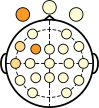
\includegraphics[width=0.13\textwidth]{./img_art_dfa/cabeza_new_MFGR_30.pdf} \\
\midrule
$30 \times 2^{-1}$ &
\includegraphics[width=0.13\textwidth]{./img_art_dfa/cabeza_new_VCR_15.pdf} &
\includegraphics[width=0.13\textwidth]{./img_art_dfa/cabeza_new_MJH_15.pdf} &
\includegraphics[width=0.13\textwidth]{./img_art_dfa/cabeza_new_JAE_15.pdf} &
\includegraphics[width=0.13\textwidth]{./img_art_dfa/cabeza_new_GHA_15.pdf} &
\includegraphics[width=0.13\textwidth]{./img_art_dfa/cabeza_new_MFGR_15.pdf} \\
\bottomrule
\end{tabular}\\
\includegraphics[scale=.7]{./img_art_dfa/escala.pdf} \\
}
\end{figure}

\begin{figure}
\centering
{\small
\begin{tabular}{lccccc}
\toprule
{ Tamaño de} & \multicolumn{5}{c}{Grupo PDC} \\
    \cmidrule{2-6}
{ ventana [s]}    & CLO & RLO & RRU & JGZ & AEFP \\
\midrule
$30 \times 2^1$ &
\includegraphics[width=0.13\textwidth]{./img_art_dfa/cabeza_new_CLO_60.pdf} &
\includegraphics[width=0.13\textwidth]{./img_art_dfa/cabeza_new_RLO_60.pdf} &
\includegraphics[width=0.13\textwidth]{./img_art_dfa/cabeza_new_RRU_60.pdf} &
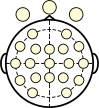
\includegraphics[width=0.13\textwidth]{./img_art_dfa/cabeza_new_JGZ_60.pdf} &
\includegraphics[width=0.13\textwidth]{./img_art_dfa/cabeza_new_AEFP_60.pdf} \\
\midrule
$30 \times 2^0$ &
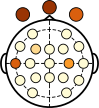
\includegraphics[width=0.13\textwidth]{./img_art_dfa/cabeza_new_CLO_30.pdf} &
\includegraphics[width=0.13\textwidth]{./img_art_dfa/cabeza_new_RLO_30.pdf} &
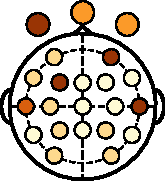
\includegraphics[width=0.13\textwidth]{./img_art_dfa/cabeza_new_RRU_30.pdf} &
\includegraphics[width=0.13\textwidth]{./img_art_dfa/cabeza_new_JGZ_30.pdf} &
\includegraphics[width=0.13\textwidth]{./img_art_dfa/cabeza_new_AEFP_30.pdf} \\
\midrule
$30 \times 2^{-1}$ &
\includegraphics[width=0.13\textwidth]{./img_art_dfa/cabeza_new_CLO_15.pdf} &
\includegraphics[width=0.13\textwidth]{./img_art_dfa/cabeza_new_RLO_15.pdf} &
\includegraphics[width=0.13\textwidth]{./img_art_dfa/cabeza_new_RRU_15.pdf} &
\includegraphics[width=0.13\textwidth]{./img_art_dfa/cabeza_new_JGZ_15.pdf} &
\includegraphics[width=0.13\textwidth]{./img_art_dfa/cabeza_new_AEFP_15.pdf} \\
\bottomrule
\end{tabular} \\
\includegraphics[scale=.7]{./img_art_dfa/escala.pdf} \\
}
\caption{Regiones donde la cantidad  de ventanas estacionarias es significativamente diferente
durante MOR y NMOR. Diferentes tamaños de ventana}
\end{figure}

%%%%%%%%%%%%%%%%%%%%%%%%%%%%%%%%%%%%%%%%%%%%%%%%%%%%%%%%%%%%%%%%%%%%%%%%%%%%%%%%%%%%%%%%%%%%%%%%%%%
%%%%%%%%%%%%%%%%%%%%%%%%%%%%%%%%%%%%%%%%%%%%%%%%%%%%%%%%%%%%%%%%%%%%%%%%%%%%%%%%%%%%%%%%%%%%%%%%%%%

\begin{figure}
\begin{subfigure}{\textwidth}
\centering
\includegraphics[width=0.9\linewidth]
{./img_ejemplos/VCNNS1_comp_est_.png} 
\caption{Épocas estacionarias usando diferentes tamaños de ventana}
\end{subfigure}
\end{figure}

\begin{figure}
\ContinuedFloat
\begin{subfigure}{\linewidth}
\centering
\includegraphics[width=0.9\linewidth]
{./enlentecimiento/VCNNS1_espectral_total.png} 
\caption{Espectro de potencias de banda ancha}
\end{subfigure}
\end{figure}

%\begin{figure}
%\ContinuedFloat
%\begin{subfigure}{\linewidth}
%\centering
%\includegraphics[width=0.9\linewidth]
%{./img_resultados/VCNNS1_combinado_.png} 
%\caption{Espectro de potencias y análisis de estacionariedad para los canales LOG, ROG y EMG}
%\end{subfigure}
%\end{figure}

\begin{figure}
\ContinuedFloat
\begin{subfigure}{\linewidth}
\centering
\includegraphics[width=.9\linewidth]{./img_resultados/cabeza_VCR.pdf}
%\caption{Porcentajes de épocas estacionarias, VCR (VCNNS1)}
\caption{Resumen de épocas estacionarias según tamaño de ventana}
\end{subfigure}
\caption{Gráficos individuales para el sujeto VCR}
\end{figure}

%%%%%%%%%%%%%%%%%%%%%%%%%%%%%%%%%%%%%%%%%%%%%%%%%

%\begin{figure}
%\centering
%\includegraphics[width=0.9\linewidth]
%{./img_ejemplos/MJNNVIGILOS_comp_est_.png} 
%\end{figure}
%
%\begin{figure}
%\centering
%\includegraphics[width=0.9\linewidth]
%{./enlentecimiento/MJNNVIGILOS_espectral_total.png} 
%\end{figure}
%
%\begin{figure}
%\centering
%\includegraphics[width=0.9\linewidth]
%{./img_resultados/MJNNVIGILOS_combinado_.png} 
%\end{figure}
%
%\begin{figure}
%\centering
%\includegraphics[width=.9\linewidth]{./img_resultados/cabeza_MJH.pdf}
%%\caption{Porcentajes de épocas estacionarias, MJH (MJNNVIGILOS)}
%\end{figure}
%
%%%%%%%%%%%%%%%%%%%%%%%%%%%%%%%%%%%%%%%%%%%%%%%%%%
%
%\begin{figure}
%\centering
%\includegraphics[width=0.9\linewidth]
%{./img_ejemplos/JANASUE_comp_est_.png} 
%\end{figure}
%\begin{figure}
%\centering
%\includegraphics[width=0.9\linewidth]
%{./enlentecimiento/JANASUE_espectral_total.png} 
%\end{figure}
%\begin{figure}
%\centering
%\includegraphics[width=0.9\linewidth]
%{./img_resultados/JANASUE_combinado_.png} 
%\end{figure}
%
%\begin{figure}
%\centering
%\includegraphics[width=.9\linewidth]{./img_resultados/cabeza_JAE.pdf}
%%\caption{Porcentajes de épocas estacionarias, JAE (JANASUE)}
%\end{figure}
%
%%%%%%%%%%%%%%%%%%%%%%%%%%%%%%%%%%%%%%%%%%%%%%%%%%
%
%\begin{figure}
%\centering
%\includegraphics[width=0.9\linewidth]
%{./img_ejemplos/GH24031950SUENO_comp_est_.png} 
%\end{figure}
%\begin{figure}
%\centering
%\includegraphics[width=0.9\linewidth]
%{./enlentecimiento/GH24031950SUENO_espectral_total.png} 
%\end{figure}
%\begin{figure}
%\centering
%\includegraphics[width=0.9\linewidth]
%{./img_resultados/GH24031950SUENO_combinado_.png} 
%\end{figure}
%
%\begin{figure}
%\centering
%\includegraphics[width=.9\linewidth]{./img_resultados/cabeza_GHA.pdf}
%%\caption{Porcentajes de épocas estacionarias, GHA (GH24031950SUEÑO)}
%\end{figure}
%
%%%%%%%%%%%%%%%%%%%%%%%%%%%%%%%%%%%%%%%%%%%%%%%%%%
%
%\begin{figure}
%\centering
%\includegraphics[width=0.9\linewidth]
%{./img_ejemplos/GURM251148SUE_comp_est_.png} 
%\end{figure}
%\begin{figure}
%\centering
%\includegraphics[width=0.9\linewidth]
%{./enlentecimiento/GURM251148SUE_espectral_total.png} 
%\end{figure}
%\begin{figure}
%\centering
%\includegraphics[width=0.9\linewidth]
%{./img_resultados/GURM251148SUE_combinado_.png} 
%\end{figure}
%
%\begin{figure}
%\centering
%\includegraphics[width=.9\linewidth]{./img_resultados/cabeza_MFGR.pdf}
%%\caption{Porcentajes de épocas estacionarias MFGR (GURM251148SUE)}
%\end{figure}
%
%%%%%%%%%%%%%%%%%%%%%%%%%%%%%%%%%%%%%%
%%%%%%%%%%%%%%%%%%%%%%%%%%%%%%%%%%%%%%
%%%%%%%%%%%%%%%%%%%%%%%%%%%%%%%%%%%%%%
%
%\begin{figure}
%\centering
%\includegraphics[width=0.9\linewidth]
%{./img_ejemplos/CLMN10SUE_comp_est_.png} 
%\end{figure}
%
%\begin{figure}
%\centering
%\includegraphics[width=0.9\linewidth]
%{./enlentecimiento/CLMN10SUE_espectral_total.png} 
%\end{figure}
%
%\begin{figure}
%\centering
%\includegraphics[width=0.9\linewidth]
%{./img_resultados/CLMN10SUE_combinado_.png} 
%\end{figure}
%
%\begin{figure}
%\centering
%\includegraphics[width=.9\linewidth]{./img_resultados/cabeza_CLO.pdf}
%%\caption{Porcentajes de épocas estacionarias, CLO (CLMN10SUE)}
%\end{figure}
%
%%%%%%%%%%%%%%%%%%%%%%%%%%%%%%%%%%%%%%
%
%\begin{figure}
%\centering
%\includegraphics[width=0.9\linewidth]
%{./img_ejemplos/RLMN10SUE_comp_est_.png} 
%\end{figure}
%\begin{figure}
%\centering
%\includegraphics[width=0.9\linewidth]
%{./enlentecimiento/RLMN10SUE_espectral_total.png}
%\end{figure}
%\begin{figure}
%\centering
%\includegraphics[width=0.9\linewidth]
%{./img_ejemplos/RLMN10SUE_comp_est_.png} 
%\end{figure}
%
%\begin{figure}
%\centering
%\includegraphics[width=.9\linewidth]{./img_resultados/cabeza_RLO.pdf}
%%\caption{Porcentajes de épocas estacionarias, RLO (RLMN10SUE)}
%\end{figure}
%
%%%%%%%%%%%%%%%%%%%%%%%%%%%%%%%%%%%%%%
%
%\begin{figure}
%\centering
%\includegraphics[width=0.9\linewidth]
%{./img_ejemplos/RRMNS_comp_est_.png} 
%\end{figure}
%
%\begin{figure}
%\centering
%\includegraphics[width=0.9\linewidth]
%{./enlentecimiento/RRMNS_espectral_total.png}
%\end{figure}
%
%\begin{figure}
%\centering
%\includegraphics[width=0.9\linewidth]
%{./img_resultados/RRMNS_combinado_.png} 
%\end{figure}
%
%\begin{figure}
%\centering
%\includegraphics[width=.9\linewidth]{./img_resultados/cabeza_RRU.pdf}
%%\caption{Porcentajes de épocas estacionarias, RRU (RRMNS)}
%\end{figure}
%
%%%%%%%%%%%%%%%%%%%%%%%%%%%%%%%%%%%%%%
%
%\begin{figure}
%\centering
%\includegraphics[width=0.9\linewidth]
%{./img_ejemplos/JGMN6SUE_comp_est_.png} 
%\end{figure}
%
%\begin{figure}
%\centering
%\includegraphics[width=0.9\linewidth]
%{./enlentecimiento/JGMN6SUE_espectral_total.png} 
%\end{figure}
%
%\begin{figure}
%\centering
%\includegraphics[width=0.9\linewidth]
%{./img_resultados/JGMN6SUE_combinado_.png} 
%\end{figure}
%
%\begin{figure}
%\centering
%\includegraphics[width=.9\linewidth]{./img_resultados/cabeza_JGZ.pdf}
%%\caption{Porcentajes de épocas estacionarias, JGZ (JGMN6SUE)}
%\end{figure}
%
%%%%%%%%%%%%%%%%%%%%%%%%%%%%%%%%%%%%%%
%%%%%%%%%%%%%%%%%%%%%%%%%%%%%%%%%%%%%%
%%%%%%%%%%%%%%%%%%%%%%%%%%%%%%%%%%%%%%
%
%%\begin{figure}
%%\centering
%%\includegraphics[width=0.9\linewidth]
%%{./img_ejemplos/FGHSUE_comp_est_.png} 
%%\end{figure}
%%\begin{figure}
%%\centering
%%\includegraphics[width=0.9\linewidth]
%%{./img_resultados/FGHSUE_espectral_total.png} 
%%\end{figure}
%%\begin{figure}
%%\centering
%%\includegraphics[width=0.9\linewidth]
%%{./img_resultados/FGHSUE_combinado_.png} 
%%\end{figure}
%%
%%\begin{figure}
%%\centering
%%\includegraphics[width=.9\linewidth]{./img_resultados/cabeza_FGH.pdf}
%%%\caption{Porcentajes de épocas estacionarias, FGH (FGHSUE)}
%%\end{figure}
%
%%%%%%%%%%%%%%%%%%%%%%%%%%%%%%%%%%%%%%
%
%%\begin{figure}
%%\centering
%%\includegraphics[width=0.9\linewidth]
%%{./img_ejemplos/MGNA5SUE_comp_est_.png} 
%%\end{figure}
%%\begin{figure}
%%\centering
%%\includegraphics[width=0.9\linewidth]
%%{./img_resultados/MGNA5SUE_espectral_total.png} 
%%\end{figure}
%%\begin{figure}
%%\centering
%%\includegraphics[width=0.9\linewidth]
%%{./img_resultados/MGNA5SUE_combinado_.png} 
%%\end{figure}
%%
%%\begin{figure}
%%\centering
%%\includegraphics[width=.9\linewidth]{./img_resultados/cabeza_MGG.pdf}
%%%\caption{Porcentajes de épocas estacionarias, MGG (MGNA5SUE)}
%%\end{figure}
%
%%%%%%%%%%%%%%%%%%%%%%%%%%%%%%%%%%%%%%
%
%%\begin{figure}
%%\centering
%%\includegraphics[width=0.9\linewidth]
%%{./img_ejemplos/EMNNS_comp_est_.png} 
%%\end{figure}
%%\begin{figure}
%%\centering
%%\includegraphics[width=0.9\linewidth]
%%{./img_ejemplos/EMNNS_comp_est_.png} 
%%\end{figure}
%%\begin{figure}
%%\centering
%%\includegraphics[width=0.9\linewidth]
%%{./img_ejemplos/EMNNS_comp_est_.png} 
%%\end{figure}
%%
%%\begin{figure}
%%\centering
%%\includegraphics[width=.9\linewidth]{./img_resultados/cabeza_EMT.pdf}
%%%\caption{Porcentajes de épocas estacionarias EMT (EMNNS)}
%%\end{figure}
%
%%%%%%%%%%%%%%%%%%%%%%%%%%%%%%%%%%%%%%
%
%%\begin{figure}
%%\bordes{1.5}
%%\begin{tabular}{l}
%%\Large{{Patrones visuales}}\\
%%\begin{tabular}{c}
%%\includegraphics[width=0.45\textwidth]
%%{./img_ejemplos/zoom_VCR.pdf}
%%\includegraphics[width=0.45\textwidth]
%%{./img_ejemplos/zoom_MJH.pdf}
%%\\
%%\includegraphics[width=0.45\textwidth]
%%{./img_ejemplos/zoom_JAE.pdf}
%%\includegraphics[width=0.45\textwidth]
%%{./img_ejemplos/zoom_GHA.pdf}
%%\\
%%\includegraphics[width=0.45\textwidth]
%%{./img_ejemplos/zoom_MFGR.pdf}
%%\end{tabular}
%%\end{tabular}
%%\end{figure}
%

\begin{figure}
\Large{\textbf{Patrones visuales}}\\
\includegraphics[width=0.95\textwidth]
{./img_ejemplos/zoom_VCR.pdf}
\end{figure}

\begin{figure}
\includegraphics[width=0.95\textwidth]
{./img_ejemplos/zoom_MJH.pdf}
\end{figure}

\begin{figure}
\includegraphics[width=0.95\textwidth]
{./img_ejemplos/zoom_JAE.pdf}
\end{figure}

\begin{figure}
\includegraphics[width=0.95\textwidth]
{./img_ejemplos/zoom_GHA.pdf}
\end{figure}


\begin{figure}
\includegraphics[width=0.95\textwidth]
{./img_ejemplos/zoom_MFGR.pdf}
\end{figure}

%%%%%%%%%%%%%%%%%%%%%%%%%%%%%%%%%%%%%%%%%%%%%%%%%%%%%%%%%%%%%%%%%%%%%%%%%%%%%%%%%%%%%%%%%%%%%%%%%%%%
%%%%%%%%%%%%%%%%%%%%%%%%%%%%%%%%%%%%%%%%%%%%%%%%%%%%%%%%%%%%%%%%%%%%%%%%%%%%%%%%%%%%%%%%%%%%%%%%%%%%
%%%%%%%%%%%%%%%%%%%%%%%%%%%%%%%%%%%%%%%%%%%%%%%%%%%%%%%%%%%%%%%%%%%%%%%%%%%%%%%%%%%%%%%%%%%%%%%%%%%%
%%%%%%%%%%%%%%%%%%%%%%%%%%%%%%%%%%%%%%%%%%%%%%%%%%%%%%%%%%%%%%%%%%%%%%%%%%%%%%%%%%%%%%%%%%%%%%%%%%%%


%%%%%%%%%%%%%%%%%%%%%%%%%%%%%%%%%%%%%%%%%%%%%%%%%%%%%%%%%%%%%%%%%%%%%%%%%%%%%%%%%%%%%%%%%%%%%%%%%%%
%%%%%%%%%%%%%%%%%%%%%%%%%%%%%%%%%%%%%%%%%%%%%%%%%%%%%%%%%%%%%%%%%%%%%%%%%%%%%%%%%%%%%%%%%%%%%%%%%%%

\bibliographystyle{bababbrv-lf}
\bibliography{referencias_estacionariedad,referencias_fisiologia,referencias_otros,referencias_mixto}%{}

%%%%%%%%%%%%%%%%%%%%%%%%%%%%%%%%%%%%%%%%%%%%%%%%%%%%%%%%%%%%%%%%%%%%%%%%%%%%%%%%%%%%%%%%%%%%%%%%%%%
%%%%%%%%%%%%%%%%%%%%%%%%%%%%%%%%%%%%%%%%%%%%%%%%%%%%%%%%%%%%%%%%%%%%%%%%%%%%%%%%%%%%%%%%%%%%%%%%%%%

\end{document}

%%%%%%%%%%%%%%%%%%%%%%%%%%%%%%%%%%%%%%%%%%%%%%%%%%%%%%%%%%%%%%%%%%%%%%%%%%%%%%%%%%%%%%%%%%%%%%%%%%%
%%%%%%%%%%%%%%%%%%%%%%%%%%%%%%%%%%%%%%%%%%%%%%%%%%%%%%%%%%%%%%%%%%%%%%%%%%%%%%%%%%%%%%%%%%%%%%%%%%%
%%%%%%%%%%%%%%%%%%%%%%%%%%%%%%%%%%%%%%%%%%%%%%%%%%%%%%%%%%%%%%%%%%%%%%%%%%%%%%%%%%%%%%%%%%%%%%%%%%%
%%%%%%%%%%%%%%%%%%%%%%%%%%%%%%%%%%%%%%%%%%%%%%%%%%%%%%%%%%%%%%%%%%%%%%%%%%%%%%%%%%%%%%%%%%%%%%%%%%%